\documentclass{article}

  % packages
    % basic stuff for rendering math
    \usepackage[letterpaper, top=1in, bottom=1in, left=1in, right=1in]{geometry}
    \usepackage[utf8]{inputenc}
    \usepackage[english]{babel}
    \usepackage{amsmath} 
    \usepackage{amssymb}
    % \usepackage{amsthm}

    % extra math symbols and utilities
    \usepackage{mathtools}        % for extra stuff like \coloneqq
    \usepackage{mathrsfs}         % for extra stuff like \mathsrc{}
    \usepackage{centernot}        % for the centernot arrow 
    \usepackage{bm}               % for better boldsymbol/mathbf 
    \usepackage{enumitem}         % better control over enumerate, itemize
    \usepackage{xr-hyper}
    \usepackage{hyperref}         % for hypertext linking
    \usepackage{fancyvrb}          % for better verbatim environments
    \usepackage{newverbs}         % for texttt{}
    \usepackage{xcolor}           % for colored text 
    \usepackage{listings}         % to include code
    \usepackage{lstautogobble}    % helper package for code
    \usepackage{parcolumns}       % for side by side columns for two column code
    

    % page layout
    \usepackage{fancyhdr}         % for headers and footers 
    \usepackage{lastpage}         % to include last page number in footer 
    \usepackage{parskip}          % for no indentation and space between paragraphs    
    \usepackage[T1]{fontenc}      % to include \textbackslash
    \usepackage{footnote}
    \usepackage{etoolbox}

    % for custom environments
    \usepackage{tcolorbox}        % for better colored boxes in custom environments
    \tcbuselibrary{breakable}     % to allow tcolorboxes to break across pages

    % figures
    \usepackage{pgfplots}
    \pgfplotsset{compat=1.18}
    \usepackage{float}            % for [H] figure placement
    \usepackage{tikz}
    \usepackage{tikz-cd}
    \usepackage{circuitikz}
    \usetikzlibrary{arrows}
    \usetikzlibrary{positioning}
    \usetikzlibrary{calc}
    \usepackage{graphicx}
    \usepackage{algorithmic}
    \usepackage{caption} 
    \usepackage{subcaption}
    \captionsetup{font=small}

    % for tabular stuff 
    \usepackage{dcolumn}

    \usepackage[nottoc]{tocbibind}
    \pdfsuppresswarningpagegroup=1
    \hfuzz=5.002pt                % ignore overfull hbox badness warnings below this limit

  % New and replaced operators
    \DeclareMathOperator*{\card}{card}
    \DeclareMathOperator{\im}{Im}
    \DeclareMathOperator{\re}{Re}
    \DeclareMathOperator*{\argmin}{\arg\!\min}
    \DeclareMathOperator*{\argmax}{\arg\!\max}
    \newcommand{\qed}{\hfill$\blacksquare$}     % I like QED squares to be black

  % Custom Environments
    \newtcolorbox[auto counter, number within=section]{question}[1][]
    {
      colframe = orange!25,
      colback  = orange!10,
      coltitle = orange!20!black,  
      breakable, 
      title = \textbf{Question \thetcbcounter ~(#1)}
    }

    \newtcolorbox[auto counter, number within=section]{exercise}[1][]
    {
      colframe = teal!25,
      colback  = teal!10,
      coltitle = teal!20!black,  
      breakable, 
      title = \textbf{Exercise \thetcbcounter ~(#1)}
    }
    \newtcolorbox[auto counter, number within=section]{solution}[1][]
    {
      colframe = violet!25,
      colback  = violet!10,
      coltitle = violet!20!black,  
      breakable, 
      title = \textbf{Solution \thetcbcounter}
    }
    \newtcolorbox[auto counter, number within=section]{lemma}[1][]
    {
      colframe = red!25,
      colback  = red!10,
      coltitle = red!20!black,  
      breakable, 
      title = \textbf{Lemma \thetcbcounter ~(#1)}
    }
    \newtcolorbox[auto counter, number within=section]{theorem}[1][]
    {
      colframe = red!25,
      colback  = red!10,
      coltitle = red!20!black,  
      breakable, 
      title = \textbf{Theorem \thetcbcounter ~(#1)}
    } 
    \newtcolorbox[auto counter, number within=section]{proposition}[1][]
    {
      colframe = red!25,
      colback  = red!10,
      coltitle = red!20!black,  
      breakable, 
      title = \textbf{Proposition \thetcbcounter ~(#1)}
    } 
    \newtcolorbox[auto counter, number within=section]{corollary}[1][]
    {
      colframe = red!25,
      colback  = red!10,
      coltitle = red!20!black,  
      breakable, 
      title = \textbf{Corollary \thetcbcounter ~(#1)}
    } 
    \newtcolorbox[auto counter, number within=section]{proof}[1][]
    {
      colframe = orange!25,
      colback  = orange!10,
      coltitle = orange!20!black,  
      breakable, 
      title = \textbf{Proof. }
    } 
    \newtcolorbox[auto counter, number within=section]{definition}[1][]
    {
      colframe = yellow!25,
      colback  = yellow!10,
      coltitle = yellow!20!black,  
      breakable, 
      title = \textbf{Definition \thetcbcounter ~(#1)}
    } 
    \newtcolorbox[auto counter, number within=section]{example}[1][]
    {
      colframe = blue!25,
      colback  = blue!10,
      coltitle = blue!20!black,  
      breakable, 
      title = \textbf{Example \thetcbcounter ~(#1)}
    } 
    \newtcolorbox[auto counter]{axiom}[1][]
    {
      colframe = green!25,
      colback  = green!10,
      coltitle = green!20!black,  
      breakable, 
      title = \textbf{Axiom \thetcbcounter ~(#1)}
    } 
    \newtcolorbox[auto counter, number within=section]{algo}[1][]
    {
      colframe = green!25,
      colback  = green!10,
      coltitle = green!20!black,  
      breakable, 
      title = \textbf{Algorithm \thetcbcounter ~(#1)}
    } 

    \definecolor{dkgreen}{rgb}{0,0.6,0}
    \definecolor{gray}{rgb}{0.5,0.5,0.5}
    \definecolor{mauve}{rgb}{0.58,0,0.82}
    \definecolor{darkblue}{rgb}{0,0,139}
    \definecolor{lightgray}{gray}{0.93}
    \renewcommand{\algorithmiccomment}[1]{\hfill$\triangleright$\textcolor{blue}{#1}}

    % default options for listings (for code)
    \lstset{
      autogobble,
      frame=ltbr,
      language=Python,
      aboveskip=3mm,
      belowskip=3mm,
      showstringspaces=false,
      columns=fullflexible,
      keepspaces=true,
      basicstyle={\small\ttfamily},
      numbers=left,
      firstnumber=1,                        % start line number at 1
      numberstyle=\tiny\color{gray},
      keywordstyle=\color{blue},
      commentstyle=\color{dkgreen},
      stringstyle=\color{mauve},
      backgroundcolor=\color{lightgray}, 
      breaklines=true,                      % break lines
      breakatwhitespace=true,
      tabsize=3, 
      xleftmargin=2em, 
      framexleftmargin=1.5em, 
      stepnumber=1
    }

  % Page style
    \pagestyle{fancy}
    \fancyhead[L]{Set Theory}
    \fancyhead[C]{Muchang Bahng}
    \fancyhead[R]{Spring 2025} 
    \fancyfoot[C]{\thepage / \pageref{LastPage}}
    \renewcommand{\footrulewidth}{0.4pt}          % the footer line should be 0.4pt wide
    \renewcommand{\thispagestyle}[1]{}  % needed to include headers in title page

  % external documents 
    \externaldocument[place-]{../Point_Set_Topology/paper}[../Point_Set_Topology/paper.pdf] 
    \externaldocument[place-]{../Real_Analysis/paper}[../Real_Analysis/paper.pdf] 

\begin{document}

\title{ZFC Set Theory}
\author{Muchang Bahng}
\date{Spring 2025}

\maketitle
\tableofcontents
\pagebreak

This covers computability theory, complexity theory, and automata theory. 
Alphabet. Boolean logic


\section{Sets} 

  So with these paradoxes in mind, we would like to construct an axiomatic formulation of sets. My take is to think that sets ``exist'' out there somewhere in the universe, and our job is to find them. Cantor with his naive set theory believed that for every meaningful property of things there is a set whose members are exactly all the things with that property. Russell shows this this cannot be the case. Nevertheless, \textit{some} sets exist, and we have intuitive experience thinking about finite sets. Therefore, the axioms of set theory are a limited list of \textit{assumptions} that we hope are true about that actually existing universe of sets. As long as they are true, then whatever we conclude from them by valid reasoning steps must also be true.\footnote{This idea is called naive Platonism.} Hence we have the following definition, which first requires the familiar property of acting like a collection of something, and then obeys the axioms we set. 
  
  \begin{definition}[Set]
    A \textbf{set} $X$ is anything 
    \begin{enumerate}
      \item that has the innate property of containing elements, and 
      \item obeys the axioms of ZFC. 
    \end{enumerate}
  \end{definition}  

  Let's first talk about the language, where they are defined formally using the axioms in the next subsection. From first-order logic, note that we have the following symbols in our alphabet $\mathcal{L}_{\mathrm{ZFC}}$. 
  \begin{enumerate}
    \item The logical connectives $\neg$, $\lor$, $\land$. 
    \item The quantifier symbols $\exists, \forall$ 
    \item Brackets $()$. 
  \end{enumerate}
  To represent sets, we also need symbols, and the membership property requires us to define a symbol for that too. 
  \begin{enumerate}
    \item A countably infinite amount of variables used for representing sets. 
    \item The set membership symbol $\in$. In fact, when we say $x \in A$, this is a proposition formed from the predicate $P(x)$. 
  \end{enumerate} 
  This is what we have to work with so far. We will construct the rest of the symbols ($=, \subset, \supset, \cup, \cap$) from the axioms. 

  Now we state the axioms, which is the foundation of ZF set theory. A question one might ask is: how do we even know for sure that these axioms aren't contradictory? The answer is that we don't, and that is why we take them as axioms rather than provable theorems. Fortunately, from the formulation in the early 20th century up until now, no contradictions have been found, and if there is one, then it would be very bad news for us.  
  
  As obvious as the axioms may seem, none of them can be rigorously proven since we need to start from a set of assumptions and some principles of logic to use some deductive reasoning. 

  \begin{axiom}[Axiom of Existence]
    There exists a set which has no elements. 
  \end{axiom}

  \begin{definition}[Empty Set]
    The \textbf{empty set} is denoted $\emptyset$.\footnote{Note that this is not determined to be unique... yet!} 
  \end{definition}

  Why do we need to axiomize what seems to be such an obvious thing? The rest of the axioms that follow talk about what we can or cannot do with sets, but this whole theory would be useless if we didn't know if there exists \textit{any} set that obeys the following axioms! Therefore, we would like to assert the existence of at least one set, namely the empty set. This asserts that our universe of discourse is not void, and so it gives us a starting set to work with, which we can build on to create more sets.   

\subsection{Axiom of Extensionality} 

  The empty set is simply described as the set containing nothing, but it can be constructed in various ways. I can describe it as the set of humans that have negative age, or the set of married bachelors. All examples of this kind describe one and the same set $\emptyset$, but we cannot yet prove this. This is why we need our second axiom, which states that a set is uniquely characterized simply by its elements. 

  \begin{axiom}[Axiom of Extensionality]
    Two sets are equal (are the same set) if they have the same elements. 
    \begin{equation}
      \forall A \forall B \big[ \forall x (x \in A \iff x \in B) \iff A = B\big]
    \end{equation}
  \end{axiom} 

  \begin{definition}[Equality]
    This axiom allows us to define the equality operator $=$, which we now add to our alphabet. 
  \end{definition} 

  \begin{theorem}[Uniqueness of Empty Set]
    The empty set is unique. 
  \end{theorem}
  \begin{proof}
    Assume that $A$ and $B$ are sets with no elements. Then it is vacuously true that every element of $A$ is an element of $B$, and vice versa. Therefore by the axiom of extensionality $A = B$. 
  \end{proof}

  This next theorem now shows that every set is uniquely characterized by its distinct elements, which aligns with our established notion that sets don't contain repeated elements. 

  \begin{theorem}[Sets Don't Contain Repeated Elements]
    Sets are unique up to distinct elements. That is, given 2 sets $A, B$, 
    \begin{equation}
      \forall x (x \in A \iff x \in B) \implies A = B
    \end{equation}
  \end{theorem} 

  As an example, we have the following: 
  \begin{equation}
    \{1, 1, 2\} = \{1, 2\} = \{1, 1, 2, 2\}
  \end{equation} 
  Though note that we don't even know if any of the sets above even exist with our axioms so far! 

\subsection{Axiom of Restricted Comprehension}

  The axiom assists us in regulating which sets are viable and which are not, preventing Russell's paradox. 

  \begin{axiom}[Axiom Schema of Restricted Comprehension]
    Given $P$ a formula with $P(x)$ specifying a property of $x$, for any set $A$, there exists a set $B$ such that $x \in B$ if and only if $x \in A$ and $P(x)$. That is, if $A$ exists, then the set, written in set-builder notation, 
    \begin{equation}
      B = \{x \in A \mid P(x) \}
    \end{equation}
    exists.\footnote{Note that this axiom does not allow the construction of entities of the more general form $\{x \mid P(x)\}$. This restriction is obviously needed to avoid Russell's paradox, hence the name \textit{restricted} comprehension. } 
  \end{axiom} 

  \begin{lemma}[Uniqueness of Restricted Commprehension]
    The set $B = \{x \in A \mid P(x) \}$ is unique, and therefore it makes sense to treat it as a unique object. 
  \end{lemma}

  The axiom of specification allows us to denote subsets. 

  \begin{definition}[Subset, Superset]
    Notationally, if $A$ is a subset of $B$, then we write $A \subset B$. Similarly, we say $A$ is a \textbf{superset} of $B$, written $A \supset B$, if $B \subset A$. 
  \end{definition} 

  We can extend this to the restriction of more sets. 

  \begin{theorem}[Existence of Binary Intersection]
    That is, if $A, B$ are sets, then there is a set $C$ such that $x \in C$ if and only if $x \in A$ and $x \in B$. This allows us to define intersection as 
    \begin{equation}
      A \cap B \coloneqq \{x \in A \mid x \in B \}
    \end{equation} 
  \end{theorem} 
  \begin{proof}
    
  \end{proof} 

  We can extend this proof to define the intersection of a set of sets. 
  
  \begin{definition}[Intersection]
    Given a nonempty\footnote{$\cap \emptyset$ is not defined since every $x$ belongs to all $A \in \emptyset$ vacuously, and so such a set would be the universal set, which does not exist.} set of sets $S$, the \textbf{intersection} $\cap S$ is the unique set satisfying $x \in \cap S$ if and only if $x \in A$ for all $A \in S$. In set builder notation, we can write 
    \begin{equation}
      \bigcap S \coloneqq \{x \in A \mid \forall B (B \in S \implies x \in B) \}
    \end{equation}
    We can also expand our notation by defining the following. 
    \begin{enumerate}
      \item Just another way of writing is 
        \begin{equation}
          \cup S = \bigcap_{A \in S} A
        \end{equation}

      \item By the axiom of extensionality, we can define 
        \begin{equation}
          A_1 \cap \ldots \cap A_n = \cap \{A_1, \ldots, A_n\}
        \end{equation}
    \end{enumerate}
  \end{definition}

  \begin{definition}[Disjoint Sets]
    Two sets $A$ and $B$ are \textbf{disjoint} if $A \cap B = \emptyset$. 
  \end{definition}

  Unfortunately, the union cannot be expressed in this specification schema, and we need a separate axiom for this. 

  \begin{definition}[Set Minus]
    We can however define set minus. Given sets $A, B$
    \begin{equation}
      A \setminus B \coloneqq \{ x \in A \mid x \not\in B \}
    \end{equation}
  \end{definition}

  \begin{definition}[Set Complement]
    Given $B$ and a subset $A \subset B$, the \textbf{complement} of $A$ with respect to $B$ is 
    \begin{equation}
      A^c \coloneqq \{ x \in B \mid x \not\in A \} = B \setminus A
    \end{equation}
  \end{definition}  

  \begin{definition}[Symmetric Difference]
    Given sets $A, B$, the \textbf{symmetric difference} between the two sets is defined 
    \begin{equation}
      A \triangle B \coloneqq (A \setminus B) \cup (B \setminus A)
    \end{equation}
  \end{definition} 

\subsection{Axiom of Pairing}

  Okay this is all great, but the only set that we have claimed the existence of is $\emptyset$, and the schema of restricted comprehension is useless in constructing any new sets since 
  \begin{equation}
    \{x \in \emptyset \mid P(x) \} = \emptyset
  \end{equation}
  for any property $P$. Starting from now, we provide more helpful axioms to construct new sets. 

  \begin{axiom}[Axiom of Pairing]
    If $A, B$ are sets, then there exists a set which contains $A$ and $B$ as elements.\footnote{For example, if $A = \{1, 2\}$ and $B = \{2, 3\}$,then $\{\{1, 2\}, \{2, 3\}\}$ exists.}
    \begin{equation}
      \forall A \forall B \exists C((A \in C) \land (B \in C))
    \end{equation}
    This allows us to construct sets from old ones. 
  \end{axiom}

  Note that clearly, this set is not necessarily unique, since there can be other elements in $C$ in addition to $A$ and $B$. 

  \begin{theorem}[Nested Sets]
    By the axiom of pairing, if we have a set $X$, then $\{X\}$ is also a set, since we can set $A = B = X$ which asserts the existence of $\{X, X\} = \{X\}$. 
  \end{theorem} 

  \begin{example}[More Sets]
    Now we have unlocked our first sets that are not the empty set! Consider the following. 
    \begin{enumerate}
      \item If $A = B = \emptyset$, then by the axiom of pairing we can get $C = \{\emptyset, \emptyset\}$, which is equal to $\{\emptyset\}$ by the axiom of extensionality. 
      \item Now we let $A = \emptyset, B = \{\emptyset\}$, and so $C = \{A, B \} = \{\emptyset, \{\emptyset\}\}$. 
    \end{enumerate}
  \end{example}

\subsection{Axiom of Union}

  \begin{axiom}[Axiom of Union] 
    For any set of sets $S$, there exists a set $U$ such that $x \in U$ if and only if $x \in A$ for some $A \in S$. 
    \begin{equation}
      \forall \mathcal{F} \exists U \forall X \forall x \big[ (x \in X \land X \in \mathcal{F}) \implies x \in U \big]
    \end{equation}
  \end{axiom}

  \begin{lemma}[Union is Unique]
    The union $U$ is unique. 
  \end{lemma}
  \begin{proof}
    Again use the axiom of extensionality. 
  \end{proof} 

  \begin{definition}[Union]
    The set $U$, is called the \textbf{union} of sets $A \in S$, denoted $\cup S$. We can also expand our notation by defining the following. 
    \begin{enumerate}
      \item Just another way of writing is 
        \begin{equation}
          \cup S = \bigcup_{A \in S} A
        \end{equation}

      \item By the axiom of extensionality, we can define 
        \begin{equation}
          A_1 \cup \ldots \cup A_n = \cup \{A_1, \ldots, A_n\}
        \end{equation}
    \end{enumerate}
  \end{definition}

  Sometimes, it is formulated alternatively as follows: For any set of sets $S$, there is a set $U$ containing every element that is a member of $S$. This does not necessarily mean that $U$ is unique, and so $\cup S$ is not defined yet. However, we can define it by using the axiom of restricted comprehension and defining 
  \begin{equation}
    \cup S \coloneqq \{ x \in A \mid \exists X (x \in X \land X \in S ) \}
  \end{equation}

  \begin{example}
    \begin{equation}
      \{\{\emptyset\}\} \cup \{\emptyset, \{\emptyset\}\} = \{\emptyset, \{\emptyset\}\}
    \end{equation}
  \end{example}

\subsection{Rules of Set Operations}

  Let's first talk about rules following the union, intersection, and set minus operators. 

  \begin{theorem}[Commutativity]
    Union and intersection are commutative. 
    \begin{align}
      A \cup B & = B \cup A \\
      A \cap B & = B \cap A
    \end{align}
  \end{theorem}

  \begin{theorem}[Associativity]
    Union and intersection are associative. 
    \begin{align}
      (A \cup B) \cup C & = A \cup (B \cup C) \\
      (A \cap B) \cap C & = A \cap (B \cap C) 
    \end{align}
  \end{theorem}

  \begin{theorem}[Distributivity]
    Given sets $A, B, C$, 
    \begin{align}
      A \cap (B \cup C) & = (A \cap B) \cup (A \cap C) \\
      A \cup (B \cap C) & = (A \cup B) \cap (A \cup C)
    \end{align}
  \end{theorem}
  \begin{proof}
    Listed. 
    \begin{enumerate}
      \item $A \cap (B \cup C) = (A \cap B) \cup (A \cap C)$. 
        \begin{enumerate}
          \item $A \cap (B \cup C) \subset (A \cap B) \cup (A \cap C)$. Assume $x \in A \cap (B \cup C)$. Then $x \in A$ and $x \in B \cup C$. If $x \in B$, then $x \in A \cap B$. If $x \in C$, then $x \in A \cap C$. Therefore, since $x \in B \cup C$, it must be the case that $x \in A \cap B$ or $x \in A \cap C$, which by definition implies $x \in (A \cap B) \cup (A \cap C)$. 

          \item $A \cap (B \cup C) \supset (A \cap B) \cup (A \cap C)$. Assume that $x \in (A \cap B) \cup (A \cap C)$. Then WLOG let $x \in A \cap B$. Then $x \in A$ and $x \in B \subset (B \cup C)$, so by definition $x \in A \cap (B \cup C)$. 
        \end{enumerate}

      \item $A \cup (B \cap C) = (A \cup B) \cap (A \cup C)$.
        \begin{enumerate}
          \item $A \cup (B \cap C) \subset (A \cup B) \cap (A \cup C)$. Assume $x \in A \cup(B \cap C)$. Then $x \in A$ or $x \in B \cap C$. If $x \in A$, then since $A \subset (A \cup B)$ and $A \subset (A \cup C)$, we have $x \in (A \cup B)$ and $x \in (A \cup C)$, which by definition means $x \in (A \cup B) \cap (A \cup C)$. If $x \not\in A$, then $x \in B \cap C \implies x \in B \subset (A \cup B)$ and $x \in C \subset (A \cup C)$, and so $x \in (A \cup B) \cap (A \cup C)$. 

          \item $A \cup (B \cap C) \supset (A \cup B) \cap (A \cup C)$. Assume $x \in (A \cup B) \cap (A \cup C)$. Then $x \in A \cup B$. If $x \in A$, then since $A \subset A \cup (B \cap C)$, $x \in A \cup (B \cap C)$. If $x \not\in A$, then $x \in B$. Since $x \in A \cup C$, $x \in C$ also. Therefore by definition $x \in (B \cap C) \subset A \cup (B \cap C) \implies x \in A \cup (B \cap C)$. 
        \end{enumerate}
    \end{enumerate}
  \end{proof}

  \begin{theorem}[DeMorgan's Laws]
    If $X$ is a set and $A, B \subset X$, then 
    \begin{align}
      X \setminus (A \cup B) & = (X \setminus A) \cap (X \setminus B) \\
      X \setminus (A \cap B) & = (X \setminus A) \cup (X \setminus B)
    \end{align}
  \end{theorem}
  \begin{proof}
    Listed. 
    \begin{enumerate}
      \item $X \setminus (A \cup B) = (A \setminus A) \cap (X \setminus B)$.
        \begin{enumerate}
          \item $X \setminus (A \cup B) \subset (A \setminus A) \cap (X \setminus B)$. Assume $x \in X \setminus (A \cup B) \iff x \in X$ and $x \not\in (A \cup B)$. Since $x \not\in (A \cup B$, $x \not\in A$ and $x \not\in B$. However, $x \in X$, so $x \not\in A \implies x \in X \setminus A$. Same goes for $B$, and so $x \in (X \setminus A) \cap (X \setminus B)$. 

          \item $X \setminus (A \cup B) \supset (A \setminus A) \cap (X \setminus B)$. Assume $x \in (X \setminus A) \cap (X \setminus B)$. Then $x \in X \setminus A \iff X \in X$ and $x \not\in A$, and $x \in X \setminus B \iff x \in X$ and $x \not\in B$. Since $x \not\in A$ and $x \not\in B$, $x \not\in A \cup B$. Combined with the fact that $x \in X$, we have $x \in X \setminus (A \cup B)$. 
        \end{enumerate}

      \item $X \setminus (A \cap B) = (A \setminus A) \cup (X \setminus B)$.
        \begin{enumerate}
          \item $X \setminus (A \cap B) \subset (A \setminus A) \cup (X \setminus B)$. Let $x \in X \setminus (A \cap B)$. Then $x \in X$ and $x \not\in A \cap B$. Since $x \not\in A \cap B$, it must be the case that at least $x \not\in A$ or $x \not\in B$. WLOG let $x \not\in A$. Then $x \in X$ and $x \not\in A \implies x \in (X \setminus A) \subset (X \setminus) \cup (X \setminus B) \implies x \in (X \setminus A) \cup (X \setminus B)$. 

          \item $X \setminus (A \cap B) \supset (A \setminus A) \cup (X \setminus B)$. WLOG let $x \in (X \setminus A)$. Then $x \in X$ and $x \not\in A$, and $x \not\in A \implies x \not\in (A \cap B) \subset A$ (contrapositive is trivial). Therefore, $x \in X$ and $x \not\in (A \cap B) \iff  x \in X \setminus (A \cap B)$. 
        \end{enumerate}
    \end{enumerate}
  \end{proof} 

  \begin{theorem}[Properties of Set Difference]
    We have the following. 
    \begin{enumerate}
      \item $A \cap (B \setminus C) = (A \cap B) \setminus C$ 
      \item $A \setminus B = \emptyset$ if and only if $A \subset B$. 
    \end{enumerate}
  \end{theorem}
  \begin{proof}
    
  \end{proof} 

  \begin{theorem}[Properties of Symmetric Difference]
    We have the following. 
    \begin{enumerate}
      \item $A \triangle A = \emptyset$
      \item $A \triangle B = B \triangle A$
      \item $(A \triangle B) \triangle C = A \triangle (B \triangle C)$
      \item $A \triangle B = (A \cup B) \setminus (A \cap B)$
    \end{enumerate}
  \end{theorem}
  \begin{proof}
    
  \end{proof} 

\subsection{Axiom of Regularity} 

  \begin{axiom}[Axiom of Regularity]
    Every non-empty set $A$ contains a member $x$ such that $A$ and $x$ are disjoint sets. 
    \begin{equation}
      \forall A \big[ A \neq \emptyset \implies \exists x (x \in A \land A \cap x = \emptyset) \big]
    \end{equation}
    This, along with the axioms of pairing and union, implies that no set is an element of itself and that every set has an ordinal rank. 
  \end{axiom}


\section{Correspondences} 

\subsection{Axiom of Power Set}

  Now that we have constructed the Von Neumann ordinals, we are allowed to do \textit{indexing}. 

  \begin{axiom}[Axiom of Power Set]
    The axiom of power set states that for any set $A$, there is a set $B$ that contains every subset of $A$. 
    \begin{equation}
      \forall A \exists B \forall S (S \subset A \implies S \in B)
    \end{equation}
    The axiom of schema of restricted comprehension is then used to define the power set as the unique subset of such $B$ containing the subset of $A$ exactly. 
    \begin{equation}
      \mathcal{P}(A) = 2^A = \{X \in B \mid X \subset A \}
    \end{equation}
  \end{axiom} 

  The existence of the power set allows us to define subfamilies of subsets of a given set, namely things such as the topology or $\sigma$-algebra. But a perhaps more important consequence is the ability to construct Cartesian products of sets. So far, a set of say $\{a, b\}$ is an \textit{unordered} pair since by the axiom of extensionality, $\{a, b\} = \{b, a\}$. We would like to consider some way to order the elements into $(a, b)$, and this ordered pair $(a, b)$ must be a set. There are many ways to do this, but the most established is to take $(a, b)$ as an element of the power set of the power set of the union of sets. 

  \begin{definition}[Cartesian Product]
    The power set axiom allows for the definition of the \textbf{Cartesian product} of two sets $A$ and $B$. Note that if $a \in A, b \in B$, then by the axiom of union $a, b \in A \cup B$ and by the axiom of power set $\{a\}, \{a, b\} \in \mathcal{P}(A \cup B)$. Therefore, using the axiom of power set again we can define
    \begin{equation}
      (a, b) \coloneqq \{\{a\}, \{a, b\}\} \in \mathcal{P}(\mathcal{P}(A \cup B))
    \end{equation} 
    and the Cartesian product is defined 
    \begin{equation}
      A \times B \coloneqq \{ (a, b) \in \mathcal{P}(\mathcal{P}(A \cup B)) \mid a \in A \land b \in B \}
    \end{equation}
    which is a valid set by the axiom schema of specification. 
  \end{definition} 

  \begin{theorem}
    $(a, b) = (a^\prime, b^\prime)$ if and only if $a = a^\prime$ and $b = b^\prime$. 
  \end{theorem}
  \begin{proof}
    The backwards implication is trivial. For the forward, let us assume that $\{\{a\}, \{a, b\}\} = \{\{a^\prime\}, \{a^\prime, b^\prime\}\}$. If $a \neq b$, then $\{a\} = \{a^\prime\}$ and $\{a, b\} = \{a^\prime, b^\prime\}$. So first $a = a^\prime$ and then $\{a, b\} = \{a, b^\prime\}$ implies $b = b^\prime$. If $a = b$, then $\{\{a\}, \{a, a\}\} = \{\{a\}\}$. So $\{a\} = \{a^\prime\}$ and $\{a\} = \{a^\prime, b^\prime\}$, and we get $a = a^\prime = b^\prime$, and so $a = a^\prime$ and $b = b^\prime$. 
  \end{proof}

  \begin{theorem}
    We have 
    \begin{equation}
      A \times (B \cup C) = (A \times B) \cup (A \times C)
    \end{equation}
  \end{theorem}

  From this we can define the Cartesian product of any finite collection of sets recursively. It is indeed the case that $(X \times Y) \times Z$ is a different set from $X \times (Y \times Z)$, but as we will see in later functions, we can define a canonical bijection between them, treating them as equivalent. Furthermore, notice that we have not defined the Cartesian product of infinite sets yet. We can define them using functions actually. 

  The definition of Cartesian products allows us to formally define \textbf{correspondences}. The most notable correspondences are \textit{functions}, \textit{order relations}, and \textit{equivalence relations}. 

  \begin{definition}[Correspondence, Relation]
    A \textbf{correspondence}, or a \textbf{binary relation}, $R$ on a set $A$ is a subset of $A \times A$. We write $aRb$ if and only if $(a,b) \in R$.\footnote{It is a way of describing precisely which two elements are related to one another.} But not all relations may be meaningful or interesting. Therefore we usually like to have certain properties on these relations, including but not limited to 
    \begin{enumerate}
      \item \textit{Reflexive}. For all $a \in A$, $aRa$
      \item \textit{Symmetric}. For all $a,b \in A$, if $aRb$ then $bRa$
      \item \textit{Antisymmetric}. For all $a,b \in A$, if $aRb$ and $bRa$ then $a=b$
      \item \textit{Transitive}. For all $a,b,c \in A$, if $aRb$ and $bRc$ then $aRc$
      \item \textit{Total}. For all $a,b \in A$, either $aRb$ or $bRa$
    \end{enumerate}
  \end{definition} 

\subsection{Functions} 

  We explore our first---and most universally used---relation. 

  \begin{definition}[Function]
    Given two sets $X, Y$, a function $f: X \rightarrow Y$ is a subset $f \subset X \times Y$ satisfying the following
    \begin{enumerate}
      \item For all $x \in X$, there exists $y \in Y$ s.t. $(x, y) \in f$.\footnote{This says that $f$ must be defined for all inputs in $X$.}
      \item For all $x \in X$ and $y, y^\prime \in Y$, if $(x, y) \in f$ and $(x, y^\prime) \in f$, then $y = y^\prime$.\footnote{In other words, $f$ must map one element to exactly one element.} 
    \end{enumerate}
    The set $X$ is said to be the \textbf{domain} and $Y$ the \textbf{codomain}. 

    \begin{figure}[H]
      \centering 
      \begin{tikzcd}
        X \arrow[r, "f"'] & Y 
      \end{tikzcd}
      \caption{A diagram representing the function $f: X \rightarrow Y$.} 
      \label{fig:function at}
    \end{figure}
  \end{definition} 

  \begin{lemma} 
    Given functions $f, g$, $f = g$ if and only if the domains of $f$ and $g$ are equal and $f(x) = g(x)$ for all $x \in \mathrm{domain}(f)$. 
  \end{lemma} 

\subsubsection{Sets Mapped Through Functions}

  \begin{definition}[Image, Preimage]
    Given some $f: X \rightarrow Y$ and $A \subset X$, the \textbf{image} of $A$ under $f$ is defined 
    \begin{equation}
      f(A) \coloneqq \{y \in Y \mid \exists x \in X (f(x) = y)\}
    \end{equation}
    Given $B \subset Y$, the \textbf{preimage} of $B$ under $f$ is defined 
    \begin{equation}
      f^{-1} (B) \coloneqq \{ x \in X \mid f(x) \in B \}
    \end{equation}
  \end{definition} 

  Now let's see how these operations behavior under functions. 

  \begin{theorem}[Preservation Under Mapping Back and Forth]
    \label{preserve_back_forth}
    Given $f: A \rightarrow B$, with $A_0, A_1 \subset A$ and $B_0, B_1 \subset B$, the following hold 
    \begin{enumerate}
      \item $A_0 \subset f^{-1} (f(A_0))$, with equality holding if $f$ is injective. 
      \item $f(f^{-1}(B_0)) \subset B_0$, with equality holding if $f$ is surjective. 
    \end{enumerate}
  \end{theorem} 
  \begin{proof} 
    Listed. 
    \begin{enumerate}
      \item Assume that $x \in A_0$. Then $f(x) \in f(A_0)$. The preimage is 
      \begin{equation}
        f^{-1} (f(A_0)) \coloneqq \{ y \in A \mid f(y) \in f(A_0) \}
      \end{equation}
      and $x$ certainly satisfies the condition that $f(x) \in f(A_0)$. Therefore $x \in f^{-1} (f(A_0))$ and so $A_0 \subset f^{-1} (f(A_0))$. 

      Now assume that $f$ is injective. It suffices to prove that $f^{-1} (f(A_0)) \subset A_0$ since the other direction is proven for all functions. We prove this by proving the contrapositive, i.e. $x \not\in A_0 \implies x \not\in f^{-1} (f(A_0))$. Suppose $x \not\in A_0 \implies f(x) \not\in f(A_0) \implies f^{-1} (f(x)) \not\subset f^{-1} (f(A_0))$ by definition of the image and preimage. But note that since $f$ is injective, $f^{-1} (f(x)) = x$.\footnote{More specifically, if we treat $x$ as the singleton set, $f(x)$ is also a singleton set by definition of a function. Since $f$ is injective, the preimage of a singleton set must be a singleton set. If it were not, then there exists $x, y$ with $x \neq y$ that maps to the same $z$, which contradicts the definition of injectivity.} and thus $x \not\in f^{-1} (f(A_0))$. 

      \item We prove this using the contrapositive. Assume that $x \not\in B_0$. Then, with abuse of notation, we have by definition of the preimage and the image $f^{-1} (x) \not\subset f^{-1} (B_0) \implies f(f^{-1} (x)) \not\subset f(f^{-1}(B_0))$. But $f (f^{-1} (x)) = \{x\}$, since we are just mapping the preimage of $x$ back across to $f$. Therefore, $x \notin f( f^{-1} (B_0))$. 

      Now assume that $f$ is surjective. It suffices to prove that $B_0 \subset f (f^{-1}(B_0))$. Assume $y \in B_0$. Since $f$ is surjective, we know that $f^{-1} (y)$ is nonempty in $A$. We can state $f^{-1}(y) \subset f^{-1} (B_0)$\footnote{The formal proof of this is given in Munkres 1.2.2.a.} which then implies $f(f^{-1} (y)) \subset f (f^{-1} (B_0))$.\footnote{Again formal proof of this given in Munkres 1.2.2.e.} But $f (f^{-1} (y)) = y$ as mentioned previously, and so $y \in f(f^{-1} (B_0))$. 
    \end{enumerate}
  \end{proof}

  \begin{example}[Counterexamples]
    To see why equality does not hold in general for the two cases, look at the counterexamples below. 
    \begin{enumerate}
      \item $A_0 \not\supset f^{-1} (f(A_0))$. 
      \item $f(f^{-1}(B_0)) \not\supset B_0$. Consider $X = Y = \{0, 1\}$ and $f: X \rightarrow Y$ defined $f(0) = f(1) = 0$. Consider $C = Y$. We have $f^{-1} (C) = f^{-1} (0) \cup f^{-1} (1) = X \cup \emptyset = X$. Then $f(f^{-1} (C)) = f(X) = \{0\} \neq C$. 
    \end{enumerate}
  \end{example}

  \begin{theorem}[Preservation Under Preimages]
    \label{preserve_preimage}
    Given $f: A \rightarrow B$, with $A_\alpha \subset A$ and $B_\alpha \subset B$, $f$ preserves the inclusion, union, intersection, and set difference under the preimage. 
    \begin{enumerate}
      \item \textit{Inclusion}. $B_0 \subset B_1 \implies f^{-1} (B_0) \subset f^{-1} (B_1)$. 
      \item \textit{Union}. $f^{-1} (\cup B_\alpha) = \cup_\alpha f^{-1} (B_\alpha)$. 
      \item \textit{Intersection}. $f^{-1} (\cap B_\alpha) = \cap_\alpha f^{-1} (B_\alpha)$.
      \item \textit{Set Difference}. $f^{-1}(B_0 \setminus B_1) = f^{-1} (B_0) \setminus f^{-1} (B_1)$. 
    \end{enumerate}
  \end{theorem} 
  \begin{proof}
    Listed. 
    \begin{enumerate}
      \item \textit{Inclusion}. If $x \in B_0$, then $f^{-1} (x) \subset A$ maps to $x$ by definition. But since $x \in B_0$, $f^{-1} (x)$ maps to a point in $B_0$, and so $f^{-1} (x) \subset f^{-1} (B_0)$. Since $B_0 \subset B_1$ by assumption, $x \in B_1$, and by the previous logic but with $B_0$ replaced by $B_1$ we have $f^{-1}(x) \subset f^{-1} (B_1)$. We have just proved that $f^{-1} (x) \in f^{-1} (B_0)  \implies f^{-1} (x) \in f^{-1} (B_1)$, and so $f^{-1} (B_0) \subset f^{-1} (B_1)$. 

      \item \textit{Union}. We prove bidirectionally. 
      \begin{enumerate}
        \item $f^{-1} (B_0 \cup B_1) \subset f^{-1} (B_0) \cup f^{-1} (B_1)$. Let $x \in f^{-1} (B_0 \cup B_1)$ which by definition of the preimage means $f(x) \in B_0 \cup B_1$. Therefore $f(x) \in B_0$ or $B_1$. Without loss of generality, let $f(x) \in B_0$. Then we have 
          \begin{equation}
            x \in f^{-1} (f(x)) \subset f^{-1} (B_0)
          \end{equation} 
          where the first inclusion comes from [Munkres 1.2.1.a] when treating $A_0 = \{x\}$, and the second subset comes from [Munkres 1.2.2.a] when treating $B_0 = \{f(x)\}, B_1 = B_1$. Therefore $x \in f^{-1} (B_0) \subset f^{-1} (B_0) \cup f^{-1} (B_1)$. 
        \item $f^{-1} (B_0) \cup f^{-1} (B_1) \subset f^{-1} (B_0 \cup B_1)$. Let $x \in f^{-1}(B_0) \cup f^{-1} (B_1)$. Without loss of generality, let $x \in f^{-1}(B_0)$ which by definition of the preimage implies $f(x) \in B_0 \subset (B_0 \cup B_1) \implies f(x) \in (B_0 \cup B_1)$. Therefore, we have 
          \begin{equation}
            x \in f^{-1} (f(x)) \subset f^{-1} (B_0 \cup B_1)
          \end{equation} 
          where the inclusion claim comes from [Munkres 1.2.1.a] when treating $A_0 = \{x\}$, and the subset claim comes from [Munkres 1.2.2.a] when treating $B_0 = \{f(x)\}, B_1 = B_0 \cup B_1$. Therefore $x \in f^{-1} (B_0 \cup B_1)$. 
      \end{enumerate}
      Therefore, $f^{-1} (B_0) \cup f^{-1} (B_1) = f^{-1} (B_0 \cup B_1)$. 

      \item \textit{Intersection}. We prove bidirectionally. 
      \begin{enumerate}
        \item $f^{-1} (B_0 \cap B_1) \subset f^{-1} (B_0) \cap f^{-1} (B_1)$. Assume $x \in f^{-1} (B_0 \cap B_1)$, which by definition of the preimage means $f(x) \in B_0 \cap B_1$. So 
          \begin{align}
            f(x) \in B_0 & \implies x \in f^{-1} (f(x)) \subset f^{-1} (B_0) \\
            f(x) \in B_1 & \implies x \in f^{-1} (f(x)) \subset f^{-1} (B_1)
          \end{align}
          where the inclusion claim comes from [Munkres 1.2.1.a] when treating $A_0 = \{x\}$, and the subset claim comes from [Munkres 1.2.2.a] when treating $f(x)$ as a singleton set. Therefore $x$ is in both of the preimages and so $x \in f^{-1} (B_0) \cap f^{-1} (B_1)$. 
        \item $f^{-1} (B_0) \cap f^{-1} (B_1) \subset f^{-1} (B_0 \cap B_1)$. Let $x \in f^{-1} (B_0) \cap f^{-1} (B_1)$. Then by definition of intersection and preimage, 
          \begin{align}
            x \in f^{-1} (B_0) & \implies f(x) \in B_0 \\
            x \in f^{-1} (B_1) & \implies f(x) \in B_1 
          \end{align} 
          and so $f(x) \in B_0 \cap B_1$ by definition of intersection. This means by definition of the preimage that $x \in f^{-1}(B_0 \cap B_1)$. 
      \end{enumerate}

      \item \textit{Set Difference}. We prove bidirectionally. 
      \begin{enumerate}
        \item $f^{-1} (B_0 \setminus B_1) \subset f^{-1} (B_0) \setminus f^{-1} (B_1)$. Let $x \in f^{-1}(B_0 \setminus B_1)$ which by definition of preimage means $f(x) \in B|0 \setminus B_1$. This implies two things. First, 
          \begin{equation}
            f(x) \in B_0 \implies x \in f^{-1} (f(x)) \subset f^{-1} (B_0)
          \end{equation}
          where the inclusion comes from [Munkres 1.2.1.a] when treating $A_0 = \{x\}$ as the single set, and the subset claim comes from [Munkres 1.2.2.a] stating that inclusions are preserved under the preimage operator. Secondly, we claim that  
          \begin{align}
            f(x) \not\in B_1 & \implies x \not\in f^{-1} (B_1)
          \end{align}
          since if $x \in f^{-1} (B_1)$, then $f(x) \in B_1$ by definition of the preimage. 

        \item $f^{-1} (B_0) \setminus f^{-1} (B_1) \subset f^{-1} (B_0 \setminus B_1)$. Let $x \in f^{-1} (B_0) \setminus f^{-1} (B_1)$. Then the following holds 
          \begin{align}
            x \in f^{-1} (B_0) & \implies f(x) \in B_0 \\
            x \not\in f^{-1} (B_1) & \implies f(x) \not\in B_1
          \end{align} 
          from the definition of the preimage and the contrapositive of its implication. Therefore $f(x) \in B_0 \setminus B_1$ which by definition of the preimage $x \in f^{-1} (B_0 \setminus B_1)$. 
      \end{enumerate}
    \end{enumerate}
  \end{proof}

  \begin{theorem}[Preservation Under Images]
    \label{preserve_image}
    Given $f: A \rightarrow B$, with $A_\alpha \subset A$ and $B_\alpha \subset B$, $f$ preserves the inclusion and union under the image, but inclusion properties for the intersection and set difference hold. 
    \begin{enumerate}
      \item \textit{Inclusion}. $A_0 \subset A_1 \implies f(A_0) \subset f(A_1)$. 
      \item \textit{Union}. $f(\cup_\alpha A_\alpha) = \cup_\alpha f(A_\alpha)$. 
      \item \textit{Intersection}. $f(\cap_\alpha A_\alpha) \subset \cap_\alpha f(A_\alpha)$, and equality holds if $f$ is injective. 
      \item \textit{Set Difference}. $f(A_0 \setminus A_1) \supset f(A_0) \setminus f(A_1)$, and equality holds if $f$ is injective. 
    \end{enumerate}
  \end{theorem} 
  \begin{proof}
    Listed. 
    \begin{enumerate}
      \item \textit{Inclusion}. Let $x \in A_0$. Then by definition of the image $f(x) \in f(A_0)$. Since $A_0 \subset A_1$, then $x \in A_1$ and it immediately follows that $f(x) \in f(A_1)$. Therefore $f(A_0) \subset f(A_1)$. 

      \item \textit{Union}. We prove bidirectionally. 
      \begin{enumerate}
        \item $f(A_0 \cup A_1) \subset f(A_0) \cup f(A_1)$. Let $y \in f(A_0 \cup A_1)$. Then by definition there exists some $x \in A_0 \cup A_1$ s.t. $f(x) = y$. WLOG let $x \in A_0$. Then by definition $y = f(x) \in f(A_0) \subset f(A_0) \cup f(A_1)$. 

        \item $f(A_0) \cup f(A_1) \subset f(A_0 \cup A_1)$. Let $y \in f(A_0) \cup f(A_1)$. WLOG $y \in f(A_0)$, and there exists some $x \in A_0$ s.t. $f(x) = y$. Since $x \in A_0$, $x \in A_0 \cup A_1$, and by definition $y = f(x) = f(A_0) \cup f(A_1)$. 
      \end{enumerate}

      \item \textit{Intersection}. Assume that $y \in f(A_0 \cap A_1)$. Then by definition there exists some $x \in A_0 \cap A_1$ s.t. $f(x) = y$. So we have 
      \begin{align}
        x \in A_0 & \implies f(x) \in f(A_0) \\
        x \in A_1 & \implies f(x) \in f(A_1)
      \end{align} 
      and therefore $y = f(x) \in f(A_0) \cap f(A_1)$. 

      To prove equality, it suffices to show that $f(A_0) \cap f(A_1) \subset f(A_0 \cap A_1)$ if $f$ is injective. Assume that $y \in f(A_0) \cap f(A_1)$. Then $y \in f(A_0)$, and so there exists an $x \in A_0$ s.t. $y = f(x) \in f(A_0)$. By the same logic there exists an $x^\prime \in A_1$ s.t. $y = f(x^\prime) \in f(A_1)$. But since $f$ is injective, this implies that $x = x^\prime$. So $x \in A_0 \cap A_1$, and so $y = f(x) \in f(A_0 \cap A_1)$. 

      \item \textit{Set Difference}. Assume that $y \in f(A_0) \setminus f(A_1)$. Since $y \in f(A_0)$, there exists some $x \in A_0$ s.t. $y = f(x)$. Since $y \not\in f(A_1)$, there exists no $x^\prime \in A_1$ s.t. $y = f(x^\prime)$.  Therefore, $x \in A_0 \setminus A_1 \implies y = f(x) \in f(A_0 \setminus A_1)$. 

      To prove equality, it suffices to show that $f(A_0 \setminus A_1) \subset f(A_0) \setminus f(A_1)$ if $f$ is injective. Assume that $y \in f(A_0 \setminus A_1)$. Then there exists some $x \in A_0 \setminus A_1$ s.t. $f(x) = y$. We claim that $x$ is unique since if there were two $x, x^\prime$, then $f(x) = f(x^\prime)$ with $x \neq x^\prime$, which means $f$ is not injective. We see that $x \in A_0 \implies y = f(x) \in f(A_0)$, and $x \not\in A_1 \implies y = f(x) \not\in f(A_1)$. Therefore, $x \in f(A_0) \setminus f(A_1)$. 
    \end{enumerate}
  \end{proof} 

  \begin{example}[Intersection Not Necessarily Preserved]
    Note that intersection is not necessarily preserved. To see why, look at the counterexample. Consider $A = \{0, 1\}, B = \{1, 2\}$, and define 
    \begin{equation}
      f(0) = f(2) = 0, f(1) = 1
    \end{equation} 
    Then $f(A) = f(B) = \{0, 1\} \implies f(A) \cap f(B) = \{0, 1\}$. On the other hand, we have $A \cap B = \{1\} \implies f(A \cap B) = \{1\}$. 
  \end{example}

\subsubsection{Composite Functions}

  \begin{definition}[Composition]
    Given functions $f: X \rightarrow Y$, $g: Y \rightarrow Z$, we define the \textbf{composite}, denoted $g \circ f$ or $g(f(\cdot))$, of $f$ and $g$ as the subset
    \begin{equation}
      g \circ f \coloneqq \{ (x, z) \in X \times Z \mid \exists y \in Y (f(x) = y \land f(y) = z) \}
    \end{equation} 
  \end{definition}

  \begin{theorem}[Compositions]
    A composite is a function. 
    \begin{figure}[H]
      \centering 
      \begin{tikzcd}
        X \arrow[r, "f"] \arrow[rd, "g \circ f"'] & Y \arrow[d, "g"] \\
        & Z
      \end{tikzcd}
      \caption{Commutative diagram representing a composition of functions.} 
      \label{fig:composition}
    \end{figure}
  \end{theorem}
  \begin{proof}
    Using the definition above, we prove the two properties. 
    \begin{enumerate}
      \item For all $x \in X$, there exists $y \in Y$ s.t. $(x, y) \in f$. Similarly, for all $y \in Y$, there exists $z \in Z$ s.t. $(y, z) \in g$. Therefore, for all $x \in X$, there exists a $y \in Y$, which follows that there exists also a $z \in Z$. Therefore $g \circ f$ is defined for all inputs in $X$. 
      \item For all $x \in X$ and $z, z^\prime \in Z$, say that $(x, z), (x, z^\prime) \in g \circ f$. Then by definition of composition there exists a $y, y^\prime \in Y$ s.t. $f(x) = y, f(y) = z$ and $f(x) = y^\prime, f(y^\prime) = z^\prime$. Since $f$ is a function, $y = y^\prime$. Since $g$ is a function, $y = y^\prime \implies z = z^\prime$. Therefore $g \circ f$ is a function. 
    \end{enumerate}
  \end{proof}

  For the computer science students, note that a function behaves precisely like functional dependencies in a relational database. A composition represents a natural join. 

  \begin{theorem}[Associativity]
    Composition is associative. That is, consider $f: Y \rightarrow Z, g: X \rightarrow Y, h: W \rightarrow X$ functions. Then 
    \begin{equation}
      (f \circ g) \circ h = f \circ (g \circ h)
    \end{equation} 
    Therefore, we write this as 
    \begin{equation}
      f \circ g \circ h
    \end{equation} 
    \begin{figure}[H]
      \centering 
      \begin{tikzcd}
        & X \arrow[r, "g"] \arrow[rrd, "g \circ h"'] & Y \arrow[rd, "h"] & \\ 
        W \arrow[ru, "f"] \arrow[rru, "g \circ f"'] & & & Z 
      \end{tikzcd}
      \caption{} 
      \label{fig:associative}
    \end{figure}
  \end{theorem}
  \begin{proof}
    Consider any $w \in W$, and let us label $x = h(w)$, $y = g(x)$, $z = f(y)$, where $x, y, z$ must be uniquely determined by $w$ since it is a function. Then, 
    \begin{align}
      ((f \circ g) \circ h) (w) & = (f \circ g) (h(w)) = (f \circ g) (x) = z  \\
      (f \circ (g \circ h)) (w) & = f ((g \circ h)(w)) = f (y) = z
    \end{align}
    and they coincide for all $w \in W$. 
  \end{proof} 

  If we are familiar with algebra, this gives the set of functions $\{f: X \rightarrow X\}$ the structure of a \textit{monoid} under composition. We can also talk about commutativity. 

  \begin{definition}[Commutativity]
    Two functions $f, g: X \rightarrow X$ are said to be \textbf{commute} if 
    \begin{equation}
      f \circ g = g \circ f
    \end{equation} 
    \begin{figure}[H]
      \centering 
      \begin{tikzcd}
        X \arrow[r, "f"] \arrow[d, "g"] & X \arrow[d, "g"] \\
        X \arrow[r, "f"] & X 
      \end{tikzcd}
      \caption{Commutative diagram representing commuting functions $f, g$. } 
      \label{fig:commutative}
    \end{figure}
  \end{definition}

  \begin{theorem}[Composition]
    Let $f: X \rightarrow Y$ and $g: Y \rightarrow Z$. 
    \begin{enumerate}
      \item $f$ injective and $g$ injective $\implies$ $g \circ f$ injective. 
      \item $f$ surjective and $g$ surjective $\implies$ $g \circ f$ surjective. 
      \item $f$ bijective and $g$ bijective $\implies$ $g \circ f$ bijective. 
    \end{enumerate}
  \end{theorem}

\subsubsection{Injective, Surjective, Bijective Functions}

  \begin{definition}[Injectivity, Surjectivity, Bijectivity]
    A function $f: X \rightarrow Y$ is said to be 
    \begin{enumerate}
      \item \textbf{injective} if $\forall x \in X, \forall x^\prime \in X \big( f(x) = f(x^\prime) \implies x = x^\prime \big)$. 
      \item \textbf{surjective} if $\forall y \in Y \exists x \in X (y = f(x))$. 
      \item \textbf{bijective} if it is injective and surjective. 
    \end{enumerate}
  \end{definition}

  \begin{definition}[Inverse Function]
    If a function $f: X \rightarrow Y$ is bijective, then there exists an \textbf{inverse function} $f^{-1}: Y \rightarrow X$ satisfying 
    \begin{equation}
      \forall x \in X \big[ f(f^{-1}(x)) = f^{-1} (f(x)) = x \big]
    \end{equation}
  \end{definition} 

  \begin{definition}[Restriction, Extension]
    If $f: X \rightarrow Y$ and $X_0 \subset X$, we define the \textbf{restriction} of $f$ to $X_0$ to be the function mapping to $Y$ whose rule is 
    \begin{equation}
      f|_{X_0} \coloneqq \{ (x, f(x)) \in f x \in X_0 \}
    \end{equation} 
    Letting $g: X_0 \rightarrow Y$, any function $f: X \supset X_0 \rightarrow Y$ satisfying $f(x) = g(x)$ for all $x \in X_0$ is said to be an \textbf{extension} of $g$ to $X$. 
  \end{definition} 

  \begin{theorem}[Injectivity/Surjectivity]
    Let $f: X \rightarrow Y$, $g: Y \rightarrow Z$, and $h = g \circ f$. The following hold: 
    \begin{enumerate}
      \item $h$ injective $\implies$ $f$ injective. 
      \item $h$ surjective $\implies$ $g$ surjective. 
      \item $h$ bijective $\implies$ $f$ injective and $g$ bijective. 
    \end{enumerate}
  \end{theorem} 

  \begin{corollary}[Bijection Equals Existence of Inverse]
    $f: X \rightarrow Y$ has a inverse function $f^{-1}: B \rightarrow A$ iff it is bijective. 
  \end{corollary}

  \begin{corollary}[Decomposition]
    Any function $h: X \rightarrow Y$ can be decomposed to the form $h = g \circ f$, where $f$ is injective and $g$ is surjective. 
  \end{corollary}
  \begin{proof}
    Given $X$, let us define an equivalence class where for any $x, y \in X$, $x \sim y$ iff $f(x) = f(y)$. Call this quotient space $X / \sim$. Then we can define the mappings. 
    \begin{enumerate}
      \item $\iota: X \rightarrow X / \sim$ which maps each element to its equivalence class. $\iota(x) = [x]$
      \item $f^\prime: X / \sim \rightarrow Y$ which maps each class to the element of $Y$ that it maps to. $f^\prime ([x]) = f(x)$. 
    \end{enumerate}
    $\iota$ is surjective since for every $[x] \in X / \sim$, there exists at least one element $x \in X$ that maps to it. $f^\prime$ is injective since have squished all the points $x$ that map to the same $y$ into a single class $[x]$. 

    \begin{figure}[H]
      \centering 
      \begin{tikzcd}
        X \arrow[r, "f"] \arrow[d, "\iota"] & Y \\
        X / \sim \arrow[ru, "f^\prime"'] & 
      \end{tikzcd}
      \caption{Decomposition of $f$ into surjective $\iota$ and injective $f^\prime$. } 
      \label{fig:decomposition}
    \end{figure}
  \end{proof}

  \begin{theorem}[Inverse of Inverses]
    If $f$ is bijective, then $f = (f^{-1})^{-1}$. 
  \end{theorem}

  \begin{theorem}[Inverse of Compositions]
    If $f, g$ are both bijective, then 
    \begin{equation}
      (f \circ g)^{-1} = g^{-1} \circ f^{-1}
    \end{equation}
  \end{theorem}

  \begin{theorem}[Finite Set Mappings]
    Suppose $X$ and $Y$ are finite sets, each with $n$ elements, and $f: X \rightarrow Y$. If $f$ is injective or bijective, then $f$ is bijective. 
  \end{theorem} 

\subsubsection{Cartesian Products as Functions} 

  Remember that we have used the power set to construct the binary Cartesian product of sets. Now we extend this to arbitrary Cartesian products using functions. 

  \begin{lemma} 
    Let $A$ and $B$ be sets. Then the set of all functions $f: A \rightarrow B$ is denoted $B^A$. We claim that this set exists. 
  \end{lemma}
  \begin{proof}
    
  \end{proof}

  \begin{definition}[Cartesian Product]
    Let $I$ be some set (used for indexing) and $S = \{S_i\}_{i \in I}$ be an indexed set of sets. Then we define the \textbf{Cartesian product} of $S_i$'s as 
    \begin{equation}
      \prod S = \prod_{i \in I} S_i \coloneqq \{f \in (\cup S)^I \mid f(i) \in S_i \; \forall i \in I \}
    \end{equation}
    Note that we need the property since we want $f(i)$ to map specifically into $S_i$. 
  \end{definition}

  With this more general construction, we can pretty much forget about the previous construction of binary Cartesian products. 

\subsection{Order Relations} 
  
  \begin{definition}[Partial Order]
    An \textbf{order} is a relation $R$, usually denoted $\leq$, that satisfies the following properties. 
    \begin{enumerate}
      \item \textit{Reflexive}. For all $a \in A$, $a \leq a$
      \item \textit{Antisymmetric}. For all $a,b \in A$, if $a \leq b$ and $b \leq a$ then $a=b$
      \item \textit{Transitive}. For all $a,b,c \in A$, if $a \leq b$ and $b \leq c$ then $a \leq c$
    \end{enumerate} 
    Note that when we say $x \leq y$, this means "$x$ is related to $y$" (but does not necessarily mean that $y$ is related to $x$), or "$x$ is less than or equal to $y$." A set $X$ with a partial order is called a partially ordered set. 
  \end{definition} 

  \begin{example}[Partially Ordered Sets]
    We list some examples of partially ordered sets. 
    \begin{enumerate}
      \item The real numbers ordered by the standard "less-than-or-equal" relation $\leq$ (totally ordered set as well). 
      \item The set of subsets of a given set $X$ ordered by inclusion. That is, the power set $2^X$ with the partial order $\subseteq$ is partially ordered. 
      \item The set of natural numbers equipped with the relation of divisibility. 
      \item The set of subspaces of a vector space ordered by inclusion. 
      \item For a partially ordered set $P$, the sequence space containing all sequences of elements from $P$, where sequence $a$ precedes sequence $b$ if every item in $a$ precedes the corresponding item in $b$. 
    \end{enumerate}
  \end{example} 

  \begin{definition}[Comparable Elements]
    Given elements $a, b$ of partially ordered set $A$, if either $a \leq b$ or $b \leq a$, then $a$ and $b$ are \textbf{comparable}. Otherwise, they are \textbf{incomparable}. 
  \end{definition}

  While partial ordering is nice, we would often want a stricter structure so that the order ``encompasses'' the whole set, i.e. every element is comparable. This property is sometimes known as \textit{totality}. 

  \begin{definition}[Total Order]
    A partial order in which every pair of elements is comparable is called a \textbf{total order}, or \textbf{linear order}. Note that from this $\leq$ relation, we can similarly define 
    \begin{enumerate}
      \item $a < b \iff (a \leq b) \land (a \neq b)$. 
      \item $a \geq b \iff \neg(a < b)$. 
      \item $a > b \iff \neg(a \leq b)$. 
    \end{enumerate} 
  \end{definition}

  Almost always when we talk about ordered sets, we mean totally ordered sets. So we will work with them by default and define following terms according to totally ordered sets. For convenience of notation, we also write $a < x < b \iff (a < x) \land (x < b)$. 

  \begin{definition}[Interval]
    Given a totally ordered set $X$, we denote the \textbf{intervals} as 
    \begin{enumerate}
      \item $(a, b) \coloneqq \{x \in X \mid a < x < b \}$
      \item $[a, b) \coloneqq \{x \in X \mid a \leq x < b \}$
      \item $(a, b] \coloneqq \{x \in X \mid a < x \leq b \}$
      \item $[a, b] \coloneqq \{x \in X \mid a \leq x \leq b \}$
    \end{enumerate}
  \end{definition} 

  \begin{definition}[Extrema]
    Given a totally ordered set $X$, 
    \begin{enumerate}
      \item $x \in X$ is a \textbf{maximum} $X$ if $y \leq x$ for all $y \in X$. 
      \item $x \in X$ is a \textbf{minimum} $X$ if $x \leq y$ for all $y \in X$. 
    \end{enumerate}
  \end{definition}

  \begin{definition}[Bounds]
    Given a totally ordered set $X$ and some subset $S \subset X$. 
    \begin{enumerate}
      \item $x \in X$ is an \textbf{upper bound} of $S$ if $x \geq y$ for all $y \in S$. 
      \item $x \in X$ is a \textbf{lower bound} of $S$ if $x \leq y$ for all $y \in S$. 
      \item $x \in X$ is a \textbf{supremum}, or \textbf{least upper bound}, of $S$ if $x$ is the minimum of the set of all upper bounds of $S$. 
      \item $x \in X$ is a \textbf{infimum}, or \textbf{greatest lower bound}, of $S$ if $x$ is the maximum of the set of all lower bounds of $S$. 
    \end{enumerate}
  \end{definition}

  Note that we have defined max/min separately from the concept of bounds. You can define the maximum of a set with just knowing the set, but the bounds require \textit{both} some subset $S$ with respect to an enclosing set $X$.\footnote{For example, it makes sense to define the maximum of a set $S = [0, 1]$ by itself, but not an upper bound for it. If $X = \mathbb{Q}$, then the supremum is $1$, but if $X$ was the set of all irrationals, then this has no supremum.} Intuitively, the main difference between the supremum/infimum and maximum/minimum is that the supremum/infimum accounts for limit points of the subset $S$. 

  \begin{definition}[Convexity on Ordered Sets]
    Given a totally ordered set $(X, \leq)$, a subset $S$ is said to be \textbf{convex} if for all $a, b \in S$, 
    \begin{equation}
      a \leq c \leq b \implies c \in S
    \end{equation}
  \end{definition}

\subsection{Equivalence Relations}

  \begin{definition}[Equivalence Relation]
    An \textbf{equivalence relation} on a set $A$ is a relation, denoted $\sim$ satisfying 
    \begin{enumerate}
      \item \textit{Reflexive}. For all $a \in A$, $a \sim a$
      \item \textit{Symmetric}. For all $a,b \in A$, if $a \sim b$ then $b \sim a$
      \item \textit{Transitive}. For all $a,b,c \in A$, if $a \sim b$ and $b \sim c$ then $a \sim c$
    \end{enumerate}
    Given an equivalence relation, we can define an \textbf{equivalence class} as 
    \begin{equation}
      [y] \coloneqq \{ x \in A \mid x \sim y \}
    \end{equation}
  \end{definition}

  \begin{definition}[Partition]
    A \textbf{partition} of a set $X$ is a collection of disjoint nonempty subset of $X$ whose union is all of $A$. 
  \end{definition} 

  \begin{theorem}[Quotient Space, Map]
    \label{partition}
    The set of equivalence classes of a set $X$ with an equivalence relation $\sim$ is a partition of $X$, denoted as the \textbf{quotient set} $X/\sim$. Therefore, the map $\iota: X \rightarrow X/\sim$ is well-defined and is called a \textbf{quotient map}. 
  \end{theorem} 
  \begin{proof}
    Assume the contrary. If $X$ has one element, then its equivalence class is $[x]$ and this is trivially proven. If $X$ has at least 2 elements, let us call them $x, y \in X$ with $x \neq y$. $[x], [y]$ are their equivalence classes. Clearly due to reflexivity, $x \in [x]$ and $y \in [y]$ and so they are nonempty. Since we assumed that this is not a partition, there exists some $z \in X$ in both $[x], [y]$. But $z \in [x] \implies z \sim x$ and $z \in [y] \implies y \sim z$. So by transitivity, $x \sim z$, meaning that $[x] = [y]$. Therefore they must be the same element of a partition. 
  \end{proof}

  \begin{example}[Circles]
    $M$ is the set of circles in $\mathbb{R}^{2}$. Given $a, b \in M$, $a \sim b$ iff the radii are equal in length. We can denote each equivalence class by $\{ r \}$, where $r$ is the length of the radius. We can define addition as 
    \begin{equation}
      \{ a \} + \{ b \} \equiv \{ a + b\}
    \end{equation}
  \end{example}


\section{Structures} 

\subsection{Algebraic Structures}

  Now sets are very boring when studying by themselves. It is often the case that we \textit{endow} a set with some additional information, which we call \textit{structure}. Consider the familiar integers, which come with certain operations such as $+$ and $\times$, along with the concepts identity elements---namely $0$ and $1$---which allows us to define (additive and multiplicative) inverses. 

  \begin{definition}[Structure]
    A \textbf{structure} on a set is some additional information on the set, such as relations, constants, and operations associated with the set. 
  \end{definition} 

  A lot of these properties depend on what operations you can do with them.  

  \begin{definition}[Operation]
    A \textbf{p-ary operation}\footnote{or called an operation of arity $p$.} $\ast$ on a set $A$ is a map 
    \begin{equation}
      \ast : A^p \longrightarrow A
    \end{equation} 
    where $A^p$ is the $p$-fold Cartesian product of $A$. In specific cases, 
    \begin{enumerate}
      \item If $p = 1$, then $\ast$ is said to be \textbf{unary}. 
      \item If $p = 2$, then $\ast$ is \textbf{binary}. 
    \end{enumerate}
    We can consider for $p > 2$ and even if $p$ is infinite.  
  \end{definition}

  \begin{definition}[Monoid]
    A \textbf{monoid} is a set $S$ with an operation $+$. 
  \end{definition}

  \begin{definition}[Group]
    
  \end{definition}

  \begin{definition}[Ring]
    
  \end{definition}

  \begin{definition}[Field]
    A \textbf{field} is an algebraic structure $(\mathbb{F}, +, \cdot)$ where 
    \begin{enumerate}
      \item $\mathbb{F}$ is an abelian group under $+$, with $0$ being the \textit{additive identity}. 
      \item $\mathbb{F} \setminus \{0\}$ is an abelian group under $\cdot$, with $1$ being the \textit{multiplicative identity}. 
      \item It connects the two operations through the \textit{distributive property}.
      \begin{equation}
        x \cdot (y + z) = x \cdot y + x \cdot z
      \end{equation}
    \end{enumerate}
  \end{definition} 

  \begin{lemma}[Left = Right Distributivity]
    Left and right distributivity are equivalent. 
    \begin{equation}
      x \cdot (y + z) = (y + z) \cdot x
    \end{equation}
  \end{lemma} 
  \begin{proof}
    \begin{align}
      x \cdot (y + z) & = x \cdot y + x \cdot z && \tag{Distributive} \\
                      & = y \cdot x + z \cdot x && \tag{Commutative} \\
                      & = (y + z) \cdot x && \tag{Distributive} 
    \end{align}
  \end{proof} 

  \begin{lemma}[Properties of Addition]
    The properties of addition hold in a field. 
    \begin{enumerate}
      \item If $x + y = x + z$, then $y = z$. 
      \item If $x + y = x$, then $y = 0$. 
      \item If $x + y = 0$, then $y = -x$. 
      \item $(-(-x)) = x$. 
    \end{enumerate}
  \end{lemma}
  \begin{proof}
    For the first, we have 
    \begin{align}
      x + y = x + z & \implies -x + (x + y) = -x + (x + z) && \tag{addition is a function} \\
                    & \implies (-x + x) + y = (-x + x) + z && \tag{$+$ is associative} \\
                    & \implies 0 + y = 0 + z && \tag{definition of additive inverse} \\
                    & \implies y = z && \tag{definition of identity}
    \end{align} 
    For the second, we can set $z = 0$ and apply the first property. For the third, we have 
    \begin{align}
      x + y = 0 & \implies -x + (x + y) = -x + 0 && \tag{addition is a function} \\
                & \implies (-x + x) + y = -x + 0 && \tag{$+$ is associative} \\
                & \implies 0 + y = -x + 0 && \tag{definition of additive inverse} \\
                & \implies y = -x && \tag{definition of identity}
    \end{align}
    For the fourth, we simply follow that if $y$ is an inverse of $z$, then $z$ is an inverse of $y$. Therefore, $-x$ being an inverse of $x$ implies that $x$ is an inverse of $-x$. $-(-x)$ must also be an inverse of $-x$. Since inverses are unique\footnote{This is proved in algebra.}, $x = -(-x)$. 
  \end{proof}

  \begin{lemma}[Properties of Multiplication]
    The properties of multiplication hold in a field. 
    \begin{enumerate}
      \item If $x \neq 0$ and $xy = xz$, then $y = z$. 
      \item If $x \neq 0$ and $xy = x$, then $y = 1$. 
      \item If $x \neq 0$ and $xy = 1$, then $y = x^{-1}$. 
      \item If $x \neq 0$, then $(x^{-1})^{-1} = x$. 
    \end{enumerate}
  \end{lemma}
  \begin{proof}
    The proof is almost identical to the first. Since $x \neq 0$, we can always assume that $x^{-1}$ exists. For the first, we have
    \begin{align}
      x y = x z & \implies x^{-1} (x y) = x^{-1} (x z) && \tag{multiplication is a function} \\
                & \implies (x^{-1} x) y = (x^{-1} x) z && \tag{$\times$ is associative} \\
                & \implies 1 y = 1 z && \tag{definition of multiplicative inverse} \\  
                & \implies y = z && \tag{definition of identity}
    \end{align}
    For the second, we can set $z = 1$ and apply the first property. For the third, we have 
    \begin{align}
      xy = 1 & \implies x^{-1} (x y) = x^{-1} 1 && \tag{multiplication is a function} \\
             & \implies (x^{-1} x) y = x^{-1} 1 && \tag{$\times$ is associative} \\
             & \implies 1 y = x^{-1} 1 && \tag{definition of multiplicative inverse} \\
             & \implies y = x^{-1} && \tag{definition of identity}
    \end{align}
    For the fourth, we simply see that $x^{-1}$ is a multiplicative inverse of both $x$ and $(x^{-1})^{-1}$ in the group $(\mathbb{F} \setminus \{0\}, \times)$, and since inverses are unique, they must be equal. 
  \end{proof}

  \begin{lemma}[Properties of Distribution]
    For any $x, y, z \in \mathbb{F}$, the field axioms satisfy 
    \begin{enumerate}
      \item $0 \cdot x = 0$.
      \item If $x \neq 0$ and $y \neq 0$, then $x y \neq 0$.
      \item $-1 \cdot x = -x$. 
      \item $(-x) y = - (xy) = x (-y)$. 
      \item $(-x) (-y) = xy$. 
    \end{enumerate}
  \end{lemma} 
  \begin{proof}
    For the first, note that 
    \begin{align}
      0 x & = (0 + 0) \cdot x = 0 x + 0x 
    \end{align}
    and subtracting $0x$ from both sides gives $0 = 0x$. For the second, we can claim that $xy \neq 0$ equivalently claiming that it will have an identity. Since $x, y \neq 0$, their inverses exists, and we claim that $(xy)^{-1} = y^{-1} x^{-1}$ is an inverse. We can see that by associativity, 
    \begin{equation}
      (y^{-1} x^{-1}) (xy) = y^{-1} (x^{-1} x) y = y^{-1} y = 1
    \end{equation} 
    For the third, we see that 
    \begin{equation}
      0 = 0 \cdot x = (1 + (-1)) \cdot x = 1 \cdot x + (-1) \cdot x = x + (-1) \cdot x 
    \end{equation}
    which implies that $-1 \cdot x$ is the additive inverse. The fourth follows immediately from the third by the associative property. For the fifth we can see that 
    \begin{align}
      (-x) (-y) & = (-1) x (-1) y && \tag{property 3} \\
                & = (-1) (-1) x y && \tag{$\times$ is commutative} \\
                & = -1 \cdot (-xy) && \tag{property 3} \\
                & = -(-xy) && \tag{property 3} \\
                & = xy && \tag{addition property 4}
    \end{align}
  \end{proof}

  Note that given a set, we can really put whatever order we want on it. However, consider the field with the following order. 
  \begin{equation}
    \mathbb{F} = \{0, 1\}, \; 0 < 1
  \end{equation} 
  This does not behave well with respect to its operations because for example if we have $0 < 1$, then adding the same element to both sides should preserve the ordering. But this is not the case since $0 + 1 = 1 > 1 + 1 = 0$. While it may be easy to define an order, we would like it to be an ordered field. 

  \begin{definition}[Ordered Ring/Field]
    An \textbf{ordered ring} is a ring that has an order satisfying 
    \begin{enumerate}
      \item $y < z \implies x + y < x + z$ for all $x \in \mathbb{F}$. 
      \item $x > 0, y > 0 \implies xy > 0$. 
    \end{enumerate}
    An \textbf{ordered field} has the same definition, and an ordered field is an ordered ring. 
  \end{definition}

  \begin{theorem}[Properties]
    In an totally ordered ring, 
    \begin{enumerate}
      \item $x > 0 \implies -x < 0$. 
      \item $x \neq 0 \implies x^2 > 0$. 
      \item If $x > 0$, then $y < z \implies xy < xz$. 
    \end{enumerate}
  \end{theorem} 
  \begin{proof}
    The first property is a single-liner 
    \begin{equation}
      0 < x \implies 0 + -x < x + -x \implies -x < 0 
    \end{equation}
    For the second property, it must be the case that $x > 0$ or $x < 0$. If $x > 0$, then by definition $x^2 > 0$. If $x < 0$, then 
    \begin{equation}
      x^2 = 1 \cdot x^2 = (-1)^2 \cdot x^2 = (-1 \cdot x)^2 = (-x)^2
    \end{equation}
    and since $-x > 0$ from the first property, we have $x^2 = (-x)^2 > 0$. For the third, we use the distributive property. 
    \begin{align}
      y < z & \implies 0 < z - y \\ 
            & \implies 0 = x 0 < x(z - y) = xz - xy \\
            & \implies xy < xz
    \end{align}
  \end{proof}

\subsection{Topological and Metric Spaces} 

  \begin{definition}[Topology]
    
  \end{definition}

  Note that an order can be used to generate an order topology, which we will define below. 

  \begin{example}[Order Topology on $\mathbb{Q}$]
    The order topology on $\mathbb{Q}$ is the topology generated by the set $\mathscr{B}$ of all open intervals 
    \begin{equation}
      (a, b) \coloneqq \{ x \in \mathbb{Q} \mid a < x < b\}
    \end{equation}
  \end{example}

  \begin{definition}[Metric]
    Given an arbitrary set $X$, a \textbf{metric} on $X$ is a function 
    \begin{equation}
      d: X \times X \rightarrow \mathbb{R}
    \end{equation}
    satisfying
  \end{definition}

\subsection{Vector Spaces}

  \begin{definition}[Vector Space]
    A vector space $V$ over a field $\mathbb{F}$ is a. 
  \end{definition}

  \begin{example}[Norm]
    Given a vector space $V$ over subfield $\mathbb{F} \subset \mathbb{C}$, the norm 
    \begin{equation}
      ||\cdot|| : V \rightarrow \mathbb{R}
    \end{equation}
  \end{example}

  \begin{example}[Inner Product]
    Given a vector space $V$ over subfield $\mathbb{F} \subset \mathbb{C}$, the \textbf{inner product} 
    \begin{equation}
      \langle \cdot, \cdot \rangle : V \times V \rightarrow \mathbb{C}
    \end{equation} 
    is a map satisfying 
  \end{example}

  \begin{definition}[Convex Sets]
    A set $S$ is convex if for every point $x, y \in S$, the point 
    \begin{equation}
      z = t x + (1 - t) y \in S
    \end{equation}
    where $0 \leq t \leq 1$. 
  \end{definition}

\subsection{Measure Spaces}



\section{The Naturals} 

\subsection{Axiom of Infinity}

  Now we attempt to try and construct the natural numbers. We start with existence of the empty set $S_0 = \emptyset = \{\}$. Now given $S_n$, we can define inductively $S_{n+1}$ through a \textit{successor function} $S$ that maps to the ``next number.''
  \begin{equation}
    S_{n+1} = S(W) \coloneqq S_n \cup \{S_n\}
  \end{equation}
  where 
  \begin{enumerate}
    \item $S_n$ exists either by induction on $n$ or from the base case where the axiom of empty set applies. 
    \item $\{S_n\}$ exists through the axiom of pairing. 
    \item $S_n \cup \{S_n\}$ exists through the axiom of union. 
  \end{enumerate} 
  Note that even though we did not talk about what $n+1$ means, we can just treat it as some elements of some indexing set. Great, so we can indeed prove that each element $S_n$ exists. This motivates the following definition. 

  \begin{definition}[Inductive Set]
    A set $I$ is called \textbf{inductive} if 
    \begin{enumerate}
      \item $0 = \{\} \in I$. 
      \item If $n \in I$, then $n + 1 = S(n) = n \cup \{n\} \in I$
    \end{enumerate} 
  \end{definition}

  Therefore, an inductive set contains $0$ and with each element, its sucessor. This makes us motivate the definition of the naturals as an inductive set which contains no other elements but the natural numbers, i.e. it is the smallest inductive set. We can express this minimal property by letting every natural number $x$ be contained in \textit{every} inductive set, leading us to the following definition. 
  \begin{equation}
    \mathbb{N} = \{x \mid x \in I \text{ for every inductive set } I \} 
  \end{equation}
  But note that this does not follow the schema of restricted specification, so we must first take some \textit{existing} inductive set $A$ and define 
  \begin{equation}
    \mathbb{N} = \{x \in A \mid x \in I \text{ for every inductive set } I \} 
  \end{equation} 
  Now the question remains of whether there are any inductive sets at all. The intuitive answer is yes, but with our axioms so far, the existence of infinite sets cannot be proven actually. The reason is that we have started out with a finite set $\emptyset$, and the construction of new sets with our axioms only allows us to create more finite sets. Therefore, while we can construct finite sets with an unbounded number of elements, we can never reach an infinite set. This is why we must axiomatically claim that a finite inductive set exists. 

  \begin{axiom}[Axiom of Infinity]
    An inductive set exists. 
  \end{axiom}

  This allows us to utilize the axiom of restricted specification to construct the primitive form of the naturals. 

  \begin{definition}[Von Neumann Ordinals] 
     The \textbf{Von Neumann ordinals} is the minimal set $X$ satisfying the axiom of infinity. It is the set containing 
    \begin{align*}
      0 & = \{\} = \emptyset \\
      1 & = \{0\} = \{\emptyset\} \\
      2 & = \{0,1\} = \{\emptyset,\{\emptyset\}\} \\
      3 & = \{0,1,2\} = \{\emptyset,\{\emptyset\},\{\emptyset,\{\emptyset\}\}\} \\
      4 & = \{0,1,2,3\} = \{\emptyset,\{\emptyset\},\{\emptyset,\{\emptyset\}\},\{\emptyset,\{\emptyset\},\{\emptyset,\{\emptyset\}\}\}\} \\
      \ldots & = \ldots 
    \end{align*} 
  \end{definition} 

  Now note that the von Neumann ordinals are not the only way to construct such a set. The \textbf{Zermelo ordinals} define the successor function to be $S(w) = \{w\}$ and state that the inductive set with this successor function exists. However, the von Neumann ordinals have the nice property that the cardinality $n$ of the set is precisely the natural number that we would like to identify it with, and the fact that a natural number $n$ contains all naturals $0, \ldots, n-1$ as elements of $n$. 

\subsection{Natural Numbers}

  From this, with a few more structures we can define the naturals as a commutative monoid with respect to both the addition and multiplication operations.

  \begin{definition}[Natural Numbers]
    \label{naturals}
    The \textbf{natural numbers} $\mathbb{N} = \{0, 1, 2, \ldots\}$ is the set of von Neumann ordinals with the following structure. 
    \begin{enumerate}
      \item \textit{Order}. The relation $\leq$ defined as 
      \begin{equation}
        m \leq n \iff m \in n
      \end{equation}
      is an order relation. 

      \item \textit{Addition} can be defined recursively with the successor function as\footnote{note that I am using $\coloneqq$ to denote that this is an \textit{identity}, not an equation to be solved.}
      \begin{align}
        n + 0 & \coloneqq n \\
        n + 1 & \coloneqq S(n) \\  
        n + S(m) & \coloneqq S(n + m)
      \end{align}

      \item \textit{Multiplication} is also defined recursively using the definition of addition.  
      \begin{align}
        n \times 0 & \coloneqq 0 \\
        n \times S(m) & \coloneqq (n \times m) + n
      \end{align}
      which is familiar to the process of adding $m$ to itself $n$ times. 

      \item \textit{Additive Identity} is $0$, following directly from the definition of addition. 
      \item \textit{Multiplicative Identity} is $1$, following directly from the definition of multiplication. 
    \end{enumerate}
  \end{definition} 

  \begin{example}[Order]
    I assert that $3 \leq 4$ since 
    \begin{equation}
      \{0, 1, 2\} = 3 \in \{0, 1, 2, 3 \} = 4
    \end{equation}
  \end{example}

  \begin{example}[Addition]
    To define $5 + 2$, we can see that 
    \begin{align}
      5 + 2 & = 5 + S(1) \\
            & \coloneqq S(5 + 1) \\
            & = S(5 + S(0)) \\
            & \coloneqq S(S(5 + 0)) \\
            & \coloneqq S(S(5)) \\
            & = S(6) \\
            & = 7
    \end{align}
  \end{example}

  \begin{example}[Multiplication]
    To define $4 \times 3$, we apply the recursive definitions 
    \begin{align}
      4 \times 3 & = 4 \times S(2) \\
                 & \coloneqq 4 \times 2 + 4 \\
                 & = 4 \times S(1) + 4 \\
                 & \coloneqq 4 \times 1 + 4 + 4 \\
                 & \coloneqq 4 \times S(0) + 4 + 4 \\
                 & = 4 \times 0 + 4 + 4 + 4 \\
                 & = 0 + 4 + 4 + 4 \\
                 & = 12
    \end{align}
  \end{example}

  \begin{theorem}[Commutative]
    $+$ and $\times$ are commutative in $\mathbb{N}$. 
  \end{theorem}

  \begin{theorem}[Associativity]
    $+$ and $\times$ are associative in $\mathbb{N}$. 
  \end{theorem}

\subsection{Induction}

  \begin{lemma}[Well Ordering Principle]
    Every nonempty subset of $\mathbb{N}$ has a minimal element. 
  \end{lemma} 
  \begin{proof}
    Take a subset $A \subset \mathbb{N}$. 
    \begin{enumerate}
      \item If $0 \in A$, the minimum is $0$. 
      \item Else if $1 \in A$, the minimum is $1$. 
      \item ...
    \end{enumerate} 
  \end{proof}

  We can use this inductive property of natural numbers to prove properties of them. Note that this can only be used to prove for finite (yet unbounded) numbers! 

  \begin{lemma}[Induction Principle]
    Given $P(n)$, a property depending on a natural number $n \in \mathbb{N}$, 
    \begin{enumerate}
      \item if $P(n_0)$ is true for some $n_0 \in \mathbb{N}$, and
      \item if for every $k \geq n_0$, $P(k)$ true implies $P(k+1)$ true, 
    \end{enumerate}
    then $P(n)$ is true for all $n \geq n_0$. 
  \end{lemma}

  \begin{lemma}[Strong Induction Principle]
    Given $P(n)$, a property depending on a positive integer $n$, 
    \begin{enumerate}
      \item if $P(n_0), P(n_0 + 1), \ldots, P(n_0 + m)$ are true for some positive integer $n_0$, and nonnegative integer $m$, and 
      \item if for every $k > n_0 + m, P(j)$ is true for all $n_0 \leq j \leq k$ implies $P(k)$ is true, 
    \end{enumerate}
    then $P(n)$ is true for all $n \geq n_0$. 
  \end{lemma} 

  \begin{theorem}[Equivalence of 3 Principles]
    The well-ordering principle, induction principle, and the strong induction principle are all equivalent. 
  \end{theorem}
  \begin{proof}
    We prove the steps. 
    \begin{enumerate}
      \item \textit{Well Ordering $\implies$ Strong Induction}. 
      \item \textit{Strong Induction $\implies$ Induction}.  
      \item \textit{Induction $\implies$ Well-Ordering}. 
    \end{enumerate}
  \end{proof}

  The idea behind the strong induction principle leads to the proof using infinite descent. Infinite descent combines strong induction with the fact that every subset of the positive integers has a smallest element, i.e. there is no strictly decreasing infinite sequence of positive integers. 

  \begin{theorem}[Infinite Descent]
    Given $P(n)$, a property depending on positive integer, assume that $P(n)$ is false for a set of integers $\mathcal{S}$. Let the smallest element of $\mathcal{S}$ be $n_0$. If $P(n_0)$ false implies $P(k)$ false, where $k < n_0$, then by contradiction $P(n)$ is true for all $n$. 
  \end{theorem} 

\subsection{Sequences and The Recursion Theorem}

  Since we have defined the naturals, we can construct a function that takes in a natural number and outputs to an arbitrary set. This is called a \textit{sequence}. 

  \begin{definition}[Sequence]
    \label{def:sequence}
    Given a nonempty set $X$, a function $f: \mathbb{N} \rightarrow X$ is called a \textit{sequence}. We usually denote it by 
    \begin{equation}
      x_1, x_2, x_3, \ldots, \qquad x_n = f(n)
    \end{equation}
    It is often shorthand written as $(x_n)$.\footnote{Note that this is different from $\{x_n\}$, which is considered a \textit{set} and is unordered.} There are two ways to define such a sequence: 
    \begin{enumerate}
      \item \textit{Explicitly}. We denote $x_n = f(n)$ in some closed form. 
      \item \textit{Recursively}. We denote $x_{n+1} = g(x_n, n)$ for all $n \in \mathbb{N}$, with some base case $x_0$. 
    \end{enumerate}
  \end{definition}

  The explicit definition gives us a well-defined sequence, but the recursive definition requires a bit more care. Given an initial condition $x_0$ and some recursive condition (similar to differential equations), such a definition is only well-formulated if there exists such a sequence (or function) that satisfies these two conditions. The recursion theorem proves both the existence and uniqueness of such an infinite sequence. 

  \begin{theorem}[Recursion Theorem]
    For any set $A$, any $a \in A$, and function $g: A \times \mathbb{N} \to A$, there exists a unique infinite sequence $f: \mathbb{N} \to A$ such that 
    \begin{enumerate}
      \item $f(0) = a$. 
      \item $f(n+1) = g(f(n), n)$ for all $n \in \mathbb{N}$. 
    \end{enumerate}
  \end{theorem}

  Sequences are particularly important in topology and analysis, where they are used as a tool to analyze properties of topological spaces or metric spaces. Since we are working in an arbitrary set, we cannot do much more than this.   


\section{The Integers and Rationals}

\subsection{Integers} 

  We then construct the integers as an ordered commutative ring that embeds $\mathbb{N}$ through a canonical ordered monoid homomorphism.  

  \begin{definition}[Integers]
    The \textbf{integers}, denoted with $\mathbb{Z}$ is constructed by defining the equivalence relation on $\mathbb{N} \times \mathbb{N}$ given by 
    \begin{equation}
      (a, b) \sim (c, d) \iff a + d = b + c
    \end{equation}
    which we can think of as $(a, b)$ being the solution to $a = x + b$. We call the quotient set $\mathbb{Z} \coloneqq (\mathbb{N} \times \mathbb{N})/{\sim}$, with the following structure. 
    \begin{enumerate}
      \item \textit{Order} defined by 
        \begin{equation} 
          [(a, b)] \leq_\mathbb{Z} [(c, d)] \iff a + d \leq_\mathbb{N} b + c 
        \end{equation}
      \item \textit{Addition}. 
        \begin{equation}
          [(a, b)] +_{\mathbb{Z}} [(c, d)] \coloneqq [(a + c, b + d)] 
        \end{equation}
      \item \textit{Multiplication}. 
        \begin{equation}
          [(a, b)] \times_{\mathbb{Z}} [(c, d)] \coloneqq [(ac + bd, ad + bc)] 
        \end{equation}

      \item \textit{Additive Identity} is $0$. 
      \item \textit{Multiplicative Identity} is $1$. 
      \item \textit{Additive Inverse} of $z = (a, b) \in \mathbb{Z}$ is denoted $-z = (b, a)$.\footnote{Since $(a, b) + (b, a) = (a + b, a + b) \sim (0, 0)$.}
    \end{enumerate}
    This makes $\mathbb{Z}$ an ordered ring. 
  \end{definition} 
  
  Note that we could have chosen other extensions, but the reason that we choose this is that it preserves the structure of $\mathbb{N}$. Even though set-theoretically, $\mathbb{N}$ and $\mathbb{Z}$ are disjoint, you can embed the naturals in the integers, which aligns with our intuition. 

  \begin{theorem}[Embedding of $\mathbb{N}$ in $\mathbb{Z}$]
    The map $f: \mathbb{N} \rightarrow \mathbb{Z}$ defined $f(n) = [(n, 0)]$ is an ordered monoid homomorphism. That is, it satisfies the following
    \begin{align}
      f(n +_{\mathbb{N}} m) & = f(n)+_{\mathbb{Z}}f(m), \\
      f(n \times_{\mathbb{N}} m) & = f(n)\times_{\mathbb{Z}}f(m) \\
      n\leq m & \iff f(n)\leq_{\mathbb{Z}} f(m)
    \end{align}
  \end{theorem}

  \begin{theorem}[Countability]
    $\mathbb{Z}$ is countably infinite. 
  \end{theorem}

\subsection{Rational Numbers} 

  Just as we have done before, we construct the rationals $\mathbb{Q}$ as an ordered field that embeds $\mathbb{Q}$ through a canonical ordered ring homomorphism. 

  \begin{definition}[Rationals]
    Given the ordered ring of integers $(\mathbb{Z}, +_{\mathbb{Z}}, \times_{\mathbb{Z}}, \leq_{\mathbb{Z}})$ the \textbf{rational numbers} $(\mathbb{Q}, +_{\mathbb{Q}}, \times_{\mathbb{Q}})$ are defined as such. 
    \begin{enumerate}
      \item $\mathbb{Q}$ is the quotient space on $\mathbb{Z} \times \mathbb{Z} \setminus \{0\}$ with the equivalence relation $\sim$ 
      \begin{equation}
        (a, b) \sim (c, d) \iff a \times_{\mathbb{Z}} d = b \times_{\mathbb{Z}} c
      \end{equation} 
      We denote this class as $(a, b)$, where $b > 0$, since if $b < 0$, we know that $(-a, -b)$ are also in this order. 

      \item The additive and multiplicative identities are 
      \begin{equation}
        0_{\mathbb{Q}} \coloneqq (0_{\mathbb{Z}}, a), \;\;\; 1_{\mathbb{Q}} \coloneqq (a, a)
      \end{equation}

      \item Addition on $\mathbb{Q}$ is defined 
      \begin{equation}
        (a, b) +_{\mathbb{Q}} (c, d) \coloneqq \big( (a \times_{\mathbb{Z}} d) +_{\mathbb{Z}} (b \times_{\mathbb{Z}} c), b \times_{\mathbb{Z}} d \big) 
      \end{equation}

      \item The additive inverse is defined 
      \begin{equation}
        -(a, b) \coloneqq (-a, b)
      \end{equation}

      \item Multiplication on $\mathbb{Q}$ is defined 
      \begin{equation}
        (a, b) \times_{\mathbb{Q}} (c, d) \coloneqq \big( a \times_{\mathbb{Z}} c, b \times_{\mathbb{Z}} d \big)
      \end{equation} 

      \item The multiplicative inverse is defined 
      \begin{equation}
        (a, b)^{-1} \coloneqq (b, a)
      \end{equation}

      \item The order $\leq_{\mathbb{Q}}$ defined on the rationals as 
      \begin{equation}
        (a, b) \leq_{\mathbb{Q}} (c, d) \iff ad \leq_{\mathbb{Z}} bc
      \end{equation}
      is a total order. 
    \end{enumerate}
  \end{definition}

  \begin{theorem}[Order on Rationals]
    The order $\leq_{\mathbb{Q}}$ defined on the rationals as 
    \begin{equation}
      (a, b) \leq_{\mathbb{Q}} (c, d) \iff ad \leq_{\mathbb{Z}} bc
    \end{equation}
    is a total order. Remember that we have defined $b, d > 0$. 
  \end{theorem}
  \begin{proof}
    We prove the three properties. 
    \begin{enumerate}
      \item Reflexive. 
      \begin{equation}
        (a, b) \leq_{\mathbb{Q}} (a, b) \iff ab \leq_{\mathbb{Z}} ab
      \end{equation} 

      \item Antisymmetric. 
      \begin{align}
        (a, b) \leq_{\mathbb{Q}} (c, d) & \implies ad \leq_{\mathbb{Z}} bc
        (c, d) \leq_{\mathbb{Q}} (a, b) & \implies bc \leq_{\mathbb{Z}} ad
      \end{align} 
      This implies that both $ad = bc$, which by definition means that they are in the same equivalence class. 

      \item Transitivity. Assume that $(a, b) \leq (c, d)$ and $(c, d) \leq (e, f)$. Then, we notice that $b, d, f > 0$ and therefore by the ordered ring property\footnote{If $a \leq b$ and $0 \leq c$, then $ac \leq bc$.} of $\mathbb{Z}$, we have 
      \begin{align}
        (a, b) \leq_{\mathbb{Q}} (c, d) & \implies ad \leq_{\mathbb{Z}} bc \implies adf \leq_{\mathbb{Z}} bcf \\ 
        (c, d) \leq_{\mathbb{Q}} (e, f) & \implies cf \leq_{\mathbb{Z}} de \implies bcf \leq_{\mathbb{Z}} bde
      \end{align}
      Therefore from transitivity of the ordering on $\mathbb{Z}$ we have $adf \leq bde$. By the ordered ring property\footnote{If $a \leq b$, then $a + c \leq b + c$.}  we have $0 \leq bde - adf = d(be - af)$. But notice that $d > 0$ from our definition of rationals, and therefore it must be the case that $0 \leq be - af \implies af \leq_{\mathbb{Z}} be$, which by definition means $(a, b) \leq_{\mathbb{Q}} (e, f)$. 
    \end{enumerate}
  \end{proof} 

  \begin{theorem}[Rationals are a Field]
    $\mathbb{Q}$ is a field. 
  \end{theorem} 
  \begin{proof}
    We do a few things. 
    \begin{enumerate}
      \item Verify the additive identity. 
      \begin{equation}
        (a, b) + (0, c) = (ac + 0b, bc) = (ac, bc) \sim (a, b)
      \end{equation}
      \item Verify the multiplicative identity. 
      \begin{equation}
        (a, b) \times (c, c) = (ac, bc) \sim (a, b)
      \end{equation}
      \item Additive inverse is actually an inverse. 
      \begin{equation}
        (a, b) + (-a, b) = (ab + (-ba), bb) = (0, bb) \sim (0, 1)
      \end{equation}
      \item Multiplicative inverse is actually an inverse. 
      \begin{equation}
        (a, b) \times (b, a) = (ab, ba) = (ab, ab) \sim (1, 1)
      \end{equation}
      \item Addition is commutative. 
      \begin{equation}
        (a, b) + (c, d) = (ad + bc, bd) = (cb + ad, bd) = (c, d) + (a, b)
      \end{equation}
      \item Addition is associative. 
      \begin{align}
        (a, b) + ((c, d) + (e, f)) & = (a, b) + (cf + de, df) \\
                                   & = (adf + bcf + bde, bdf) \\
                                   & = (ad + bc, bd) + (e, f) \\
                                   & = ((a, b) + (c, d)) + (e, f)
      \end{align}
      \item Multiplication is commutative. 
      \begin{equation}
        (a, b) \times (c, d) = (ac, bd) = (ca, db) = (c, d) \times (a, b)
      \end{equation}
      \item Multiplication is associative. 
      \begin{align}
        (a, b) \times ((c, d) \times (e, f)) & = (a, b) \times (ce, df) \\ 
                                             & = (ace, bdf) \\
                                             & = (ac, bd) \times (e, f) \\
                                             & = ((a, b) \times (c, d)) \times (e, f)
      \end{align}
      \item Multiplication distributes over addition. 
        \begin{align}
          (a, b) \times ((c, d) + (e, f)) & = (a, b) \times (c, d) + (a, b) \times (e, f) \\
                                          & = (ac, bd) + (ae, bf) \\
                                          & = (abcf + abde, b^2 df) \\
                                          & = (acf + ade, bdf)  
                                          & = (a, b) \times (cf + de, df)
        \end{align}
    \end{enumerate}
  \end{proof} 

  \begin{theorem}[Rationals are an Ordered Field]
    $\mathbb{Q}$ is an ordered field. 
  \end{theorem}
  \begin{proof}
    We show that our defined order satisfies the definition. 
    \begin{enumerate}
      \item Assume that $y = (a, b) \leq (c, d) = z$. Let $x = (e, f)$. Then $x + y = (af + be, bf)$, $x + z = (cf + de, df)$. Therefore 
      \begin{align}
        (af + be) df & = adf^2 + bedf \\ 
                     & \leq bcf^2 + bedf \\
                     & = (cf + de) bf
      \end{align} 
      But $(af + be) df = (cf + de) bf$ is equivalent to saying $(af + be, bf) \leq_{\mathbb{Q}} (cf + de, df)$, i.e. $x + y \leq x + z$!  

      \item Let $x = (a, b), y = (c, d)$. Since $0 < x, 0 < y$, by construction this means that $0 < a, 0 < c$ (since $b, d > 0$ in the canonical rational form). By the ordered ring property of the integers, $0 < ac$. So 
      \begin{equation}
        0 < ac \iff 0 \cdot bd < ac \cdot 1 \iff (0, 1) < (ac, bd)  \iff 0_{\mathbb{Q}} < (a, c) \times_{\mathbb{Q}} (b, d) = x y
      \end{equation}
    \end{enumerate}
  \end{proof}

  We have successfully defined the rationals, but now these are almost completely separate elements. We know that all integers are rational numbers, and so to show that the rationals are an extension of $\mathbb{Z}$ we want to identify a \textit{canonical injection} $\iota: \mathbb{Z} \rightarrow \mathbb{Q}$. This can't just be any canonical injection; it must preserve the both the order and algebraic structure between the two sets and must therefore be a \textit{ordered ring homomorphism}. 

  \begin{theorem}[Canonical Injection of $\mathbb{Z}$ to $\mathbb{Q}$ is an Ordered Ring Homomorphism]
    Let us define the canonical injection $\iota: \mathbb{Z} \rightarrow \mathbb{Q}$ to be $\iota(a) = (a, 1)$. This is a ring homomorphism. 
  \end{theorem}
  \begin{proof} 
    We show a few things. 
    \begin{enumerate}
      \item Preservation of addition. 
        \begin{align}
          \iota(a) +_{\mathbb{Q}} \iota(b) & = (a, 1) +_{\mathbb{Q}} (b, 1) \\
                                           & = (1a +_{\mathbb{Z}} 1b, 1^2) \\
                                           & = (a +_{\mathbb{Z}} b, 1) \\
                                           & = \iota(a +_{\mathbb{Z}} b) 
        \end{align}
      \item Preservation of multiplication. 
        \begin{align}
          \iota(a) \times_{\mathbb{Q}} \iota(b) & = (a, 1) \times_{\mathbb{Q}} (b, 1) \\
                                                & = (a \times_{\mathbb{Z}} b, 1^2) \\
                                                & = (a \times_{\mathbb{Z}} b, 1) \\
                                                & = \iota(a \times_{\mathbb{Z}} b, 1)
        \end{align}
      \item Preservation of multiplicative identity. 
        \begin{equation}
          \iota(1_{\mathbb{Z}}) = (1, 1) = 1_{\mathbb{Q}}
        \end{equation}

      \item Preservation of order. 
      \begin{align}
        a \leq_{\mathbb{Z}} b & \iff a \cdot 1 \leq_{\mathbb{Z}} b \cdot 1 \\
                              & \iff (a, 1) \leq_{\mathbb{Q}} (b, 1) \\
                              & \iff \iota(a) \leq_{\mathbb{Q}} \iota(b)
      \end{align}
    \end{enumerate}
  \end{proof} 

  \begin{theorem}[Rational Numbers]
    $\mathbb{Q}$ is countable. 
  \end{theorem}
  \begin{proof}
    Since $\mathbb{N} \approx \mathbb{Z}$, it suffices to prove that $\mathbb{N} \times \mathbb{N}$ is countable. We wish to find the bijection $f: \mathbb{N} \times \mathbb{N} \rightarrow \mathbb{N}$. We claim that 
    \begin{equation}
      f(x, y) = \frac{1}{2} \big\{ (x + y - 1)^2 - (x + y - 1) + 2 \big\} + x - 1
    \end{equation}
    \begin{figure}[H]
      \centering 
      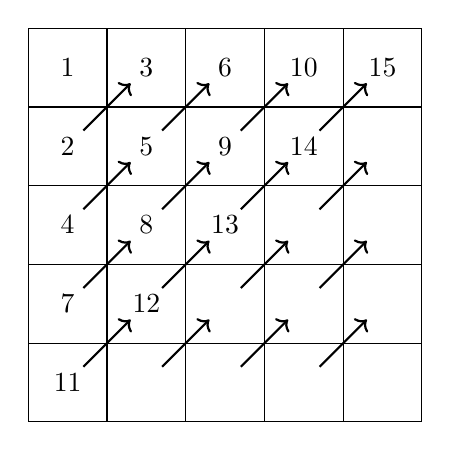
\begin{tikzpicture}[scale=1]
        % Grid
        \draw (0,0) grid (5,5);
        
        % Numbers specified (top-right triangle)
        \node at (0.5,4.5) {1};
        \node at (1.5,4.5) {3};
        \node at (2.5,4.5) {6};
        \node at (3.5,4.5) {10};
        \node at (4.5,4.5) {15};
        
        \node at (0.5,3.5) {2};
        \node at (1.5,3.5) {5};
        \node at (2.5,3.5) {9};
        \node at (3.5,3.5) {14};
        
        \node at (0.5,2.5) {4};
        \node at (1.5,2.5) {8};
        \node at (2.5,2.5) {13};
        
        \node at (0.5,1.5) {7};
        \node at (1.5,1.5) {12};
        
        \node at (0.5,0.5) {11};
        
        % Diagonal arrows
        \foreach \x in {0,...,3} {
            \foreach \y in {0,...,3} {
                \draw[->, thick] (\x+0.7,\y+0.7) -- (\x+1.3,\y+1.3);
            }
        }
      \end{tikzpicture}
      \caption{You can see that given $(x, y)$ it is on the $(x+y+1)$th diagonal, which starts from the $\frac{1}{2} \big((x+y+1)^2 - (x+y+1) + 2)$th number and increments by $x-1$. Therefore, we have the formula above. } 
      \label{fig:rationals_countable}
    \end{figure}
  \end{proof}

  \begin{theorem}[Finite Fields]
    There are no finite ordered fields. 
  \end{theorem} 
  \begin{proof}
    Assume $\mathbb{F}$ is such an ordered field. It must be the case that $0, 1 \in \mathbb{F}$, with $0 < 1$. Therefore, we also have $0 + 1 < 1 + 1 \implies 1 < 1 + 1$. Repeating this we get 
    \begin{equation}
      0 < 1 < 1 + 1 < 1 + 1 + 1 < \ldots
    \end{equation}
    where these elements must be distinct (since only one of $>, <, =$ must be true for a totally ordered set). Since this can be done for a countably infinite number of times, $\mathbb{F}$ cannot be finite. 
  \end{proof}

\subsubsection{Norm, Metric, and Topology on Rationals}

  Note that we can also define a norm on the rationals with just the order and algebraic properties. 

  \begin{theorem}[Norm on $\mathbb{Q}$] 
    The following is indeed a norm on $\mathbb{Q}$. 
    \begin{equation}
      |x| \coloneqq \begin{cases} x & \text{ if } x \geq 0 \\ -x & \text{ if } x < 0 \end{cases}
    \end{equation} 
  \end{theorem} 

  It is well known that the metric induced by any norm is indeed a metric. Therefore we state the metric as a definition. 

  \begin{definition}[Metric on $\mathbb{Q}$]
    The Euclidean metric on $\mathbb{Q}$ is defined 
    \begin{equation}
      d(x, y) \coloneqq |x - y| = \begin{cases} x - y & \text{ if } x \geq y \\ y - x & \text{ if } x < y \end{cases}
    \end{equation}
  \end{definition}

  Thus we get to what we want: the induced topology of open balls. 
  Again, since we know from point-set topology that metric topologies are indeed topologies, we will state this as a definition rather than a theorem.  

  \begin{definition}[Open-Ball Topology on $\mathbb{Q}$]
    The Euclidean topology on $\mathbb{Q}$ is the topology generated by the set $\mathscr{B}$ of all open balls
    \begin{equation}
      B(x, r) \coloneqq \{ y \in \mathbb{Q} \mid |x - y| < r \}
    \end{equation} 
  \end{definition}

  Note that this is the same topology as the order topology. This should however be proved. 

  \begin{theorem}[Metric and Order Topologies on $\mathbb{Q}$]
    The metric and order topologies on $\mathbb{Q}$ are the same topologies. 
  \end{theorem}
  \begin{proof}
    
  \end{proof}


\section{The Real Numbers}

  By constructing $\mathbb{Q}$ and its topology in my algebra and topology notes, we can talk about convergence. The first question to ask (if you were the first person inventing the reals) is ``how do I know that there exists some other numbers at all?'' The first clue is trying to find the side length of a square with area $2$. As we see, this number is not rational. 

  \begin{theorem}[$\sqrt{2}$ is Not Rational]
    \label{thm:sqrt2-irrational}
    There exists no $x \in \mathbb{Q}$ s.t. $x^2 = 2$. 
  \end{theorem}
  \begin{proof}
    Assume such a number $x = p/q$ exists, where $\mathrm{gcd}(p, q) = 1$. Then, by the field axioms of $\mathbb{Q}$, we can deduce that 
    \begin{equation}
      2 = \frac{p^2}{q^2} \implies 2 q^2 = p^2
    \end{equation}
    This implies that $2 \mid p$, so we have $p = 2p_0$, and we can write $2 q^2 = 4 p_0^2$. Dividing both sides by $2$, we get $q^2 = 2p_0^2$, which implies that $2 \mid q$. This contradicts the fact that $p$ and $q$ are coprime. 
  \end{proof} 

  We can ``imagine'' that a square with area $2$ certainly exists, but the fact that its side length is undefined is certainly unsettling. I don't know about you, but I would try to ``invent'' $\sqrt{2}$. We can do this in 4 distinct ways, though some may be more similar than others. 

  \begin{enumerate}
    \item \textit{Dedekind Completeness}. I would try and generate new elements by taking a specific \textit{cut}---a partition into two sets such that elements of one set is always greater than that of the other---and seeing which elements lie right in between these cuts. We will often see that we can always find a cut for every rational, but there are additional cuts for each irrational number. This is the idea behind \textit{Dedekind completeness}. 

    \item \textit{Cauchy Completeness}. I write out the decimal expansion one by one, which gives our first exposure to sequences. 
    \begin{equation}
      1, 1.4, 1.41, 1.414, \ldots
    \end{equation} 
    It is clear that on $\mathbb{Q}$, this sequence does not converge. Our intuition tells that that if the terms get closer and closer to each other, they must be getting closer and closer to \textit{something}, though that something is not in $\mathbb{Q}$. This motivates the definition for \textit{Cauchy completeness}. 

    \item \textit{Nested Interval Completeness}. I would write out maybe some nested intervals so that $\sqrt{2}$ \textit{must} lie within each interval. 
    \begin{equation}
      [1, 2] \supset [1.4, 1.5] \supset [1.41, 1.42] \supset \ldots 
    \end{equation}
    This motivates the definition of \textit{nested-interval completeness}. 

    \item \textit{Least Upper Bound Completeness}. I would define the set of all rationals such that $x^2 < 2$, and try to define $\sqrt{2}$ as the max or supremum of this set. We will quickly find that neither the max nor the supremum exists in $\mathbb{Q}$, and this motivates the definition for \textit{least upper bound completeness}. 
  \end{enumerate}

  All four of these methods points at the same intuition that there should not be any ``gaps'' or ``missing points'' in the set that we will construct to be $\mathbb{R}$, which is the general notion of \textit{completeness}. This contrasts with the rational numbers, whose corresponding number line has a "gap" at each irrational value. Even though constructing the reals with one method is sufficient, knowing the different flavors in which completeness manifests is very useful. It allows us to view properties of $\mathbb{R}$ through different lens. 

  The main division between these four properties is that the first two are methods to directly \textit{construct} the reals from $\mathbb{Q}$, while the latter two are more \textit{axiomatic properties} that we use to verify completeness for a given set. In the next two sections, we will take the rationals and add on extra elements using Dedekind cuts and Cauchy sequences. However, it isn't as conventional (though possible) to construct them as the single point contained in a sequence of nested intervals nor as a supremum of all upper-bounded sets. In fact, an alternative way to construct the reals is to define it axiomatically---as a totally ordered field with either the LUB property or the nested interval property.\footnote{In fact, you also need the Archimidean principle, but we'll talk about this later.} 

  Therefore, in the following sections, we will 
  \begin{enumerate}
    \item first define the relevant notion of completeness, 
    \item show that the rationals are not complete 
    \item and then construct the completed version of the rationals as a version of the reals. 
  \end{enumerate}
  Once we have done this for all three versions, we will unify them by proving they are all equivalent. 

  There is a second essential property of the reals that is not talked about as often is the Archimidean principle. 

  \begin{definition}[Archimidean Principle]
    An ordered ring $(X, +, \cdot, \leq)$ that embeds the naturals $\mathbb{N}$\footnote{as in, there exists an ordered ring homomorphism $\iota: \mathbb{N} \rightarrow X$} is said to obey the \textbf{Archimedean principle} if given any $x, y \in X$ s.t. $x, y > 0$, there exists an $n \in \mathbb{N}$ s.t. $\iota(n) \cdot x > y$. Usually, we don't care about the canonical injection and write $nx > y$. 
  \end{definition} 
  
  \begin{lemma}[Rationals are Archimidean]
    $\mathbb{Q}$ satisfies the Archimidean principle. 
  \end{lemma}
  \begin{proof}
    Take any $x = p_1/q_1, y = p_2 / q_2 \in \mathbb{Q}$. Then, take $n = q_1 p_2$, and we get 
    \begin{equation}
      n x = q_1 p_2 \frac{p_1}{q_1} = p_1 p_2 > \frac{p_2}{q_2} = y \iff p_1 > \frac{1}{q_2}
    \end{equation}
    which must be true since $p_1 \geq 1 \geq \frac{1}{q_2}$. 
  \end{proof}

  Usually, we just construct $\mathbb{R}$ right out of $\mathbb{Q}$, and it turns out that the Archimidean principle just trivially follows. However, if we construct $\mathbb{R}$ axiomatically (without the rationals), it needs to be stated. In this axiomatic formulation, we will find that certain types of completeness---like Dedekind completeness---actually \textit{implies} the Archimidean principle, while others---like Cauchy and nested-intervals completeness---does not. Therefore, in a sense, Dedekind completeness is the ``strongest'' form of completeness. 

\subsection{Dedekind Completeness}  

  This is an explicit construction from the rationals. 

  \begin{definition}[Dedekind Cut] 
    A \textbf{Dedekind cut} is a partition of the rationals $\mathbb{Q} = A \sqcup A^\prime$ satisfying the three properties.\footnote{This can really be defined for any totally ordered set. } 
    \begin{enumerate}
      \item $A \neq \emptyset$ and $A \neq \mathbb{Q}$.\footnote{By relaxing this property, we can actually complete $\mathbb{Q}$ to the extended real number line. }
      \item $x < y$ for all $x \in A, y \in A^\prime$. 
      \item The maximum element of $A$ does not exist in $\mathbb{Q}$. 
    \end{enumerate}
    The minimum of $A^\prime$ may exist in $\mathbb{Q}$, and if it does, the cut is said to be \textbf{generated} by $\min A^\prime$. 
  \end{definition}

  Note that in $\mathbb{Q}$, there will be two types of cuts: 
  \begin{enumerate}
    \item ones that are generated by rational numbers, such as 
    \begin{equation}
      A = \{x \in \mathbb{Q} \mid x < 2/3 \}, A^\prime = \{ x \in \mathbb{Q} \mid x \geq 2/3 \} 
    \end{equation}
    \item and the ones that are not 
    \begin{equation}
      A = \{x \in \mathbb{Q} \mid x^2 < 2 \}, A^\prime = \{x \in \mathbb{Q} \mid x^2 \geq 2 \}
    \end{equation}
  \end{enumerate}
  We can intuitively see that the set of all Dedekind cuts $(A, A^\prime)$ will ``extend'' the rationals into a bigger set. We can then define some operations and an order to construct this into an ordered field, and finally it will have the property that we call ``completeness.''

  \begin{definition}[Dedekind Completeness]
    A totally ordered algebraic field $\mathbb{F}$ is \textbf{Dedekind-complete} if every Dedekind cut of $\mathbb{F}$ is generated by an element of $\mathbb{F}$. 
  \end{definition}

  \begin{lemma}[Rationals are Not Dedekind-Complete]
    $\mathbb{Q}$ is not Dedekind-complete. 
  \end{lemma}
  \begin{proof}
    Take a look at the cut
    \begin{equation}
      A = \{x \in \mathbb{Q} \mid x^2 < 2 \}, A^\prime = \{x \in \mathbb{Q} \mid x^2 \geq 2 \}
    \end{equation}
    We wish to show that $A^\prime$ has no minimum. Assume that it does, and call it $p$. Then, define 
    \begin{equation}
      q \coloneqq p - \frac{p^2 - 2}{p + 2} = \frac{2p + 2}{p + 2} 
    \end{equation}
    We can see that $p > 2 \implies p^2 - 2 > 0 \implies q < p$. But we also see that 
    \begin{equation}
      q^2 - 2 = \frac{2 (p^2 - 2)}{(p + 2)^2} \implies q^2 > 2
    \end{equation}
    Therefore, we have found a $q \in A^\prime$ that is smaller than $p$, a contradiction. 
  \end{proof}

  These Dedekind cuts are simply subsets of the power set of $\mathbb{Q}$, which always exists due to the \hyperref[st-power-set-axiom]{power set axiom}. Therefore, we can simply use the axiom of restricted comprehension (?) to create a well-defined set of Dedekind cuts.    

  \begin{definition}[Reals as the Dedekind-Completion of Rationals]
    Let $\mathbb{R}_D$ be the set of all Dedekind cuts $A$\footnote{For convenience we can uniquely represent $(A, A^\prime)$ with just $A$ since $A^\prime = \mathbb{Q} \setminus A$. }  of $\mathbb{Q}$. 

    \begin{equation}
      \mathbb{R}_D \coloneqq \{ A \in 2^{\mathbb{Q}} \mid (A, A^c) \text{ is a Dedekind cut}\}
    \end{equation}
    By doing this we can intuitively think of a real number as being represented by the set of all smaller rational numbers. Let $A, B \in \mathbb{R}_D$ two Dedekind cuts. Then, we define the following order and operations. 
    \begin{enumerate}
      \item \textit{Order}. $A \leq_{\mathbb{R}} B \iff A \subset B$. 
      \item \textit{Addition}. $A +_{\mathbb{R}} B \coloneqq \{ a +_{\mathbb{Q}} b \mid a \in A, b \in B \}$. 
      \item \textit{Additive Identity}. $0_{\mathbb{R}} \coloneqq \{x \in \mathbb{Q} \mid x < 0 \}$. 
      \item \textit{Additive Inverse}. $-B \coloneqq \{ a - b \mid a < 0 , b \in (\mathbb{Q} \setminus B) \}$.
      \item \textit{Multiplication}. If $A, B \geq 0$, then we define $A \times_{\mathbb{R}} B \coloneqq \{ a \times_{\mathbb{Q}} b \mid a \in A, b \in B, a, b \geq 0\} \cup 0_{\mathbb{R}}$. If $A$ or $B$ is negative, then we use the identity $A \times B = -(A \times_{\mathbb{R}} -B) = -(-A \times_{\mathbb{R}} B) = (-A \times_{\mathbb{R}} -B)$ to convert $A, B$ to both positives and apply the previous definition. 
      \item \textit{Multiplicative Identity}. $1_{\mathbb{R}} = \{x \in \mathbb{Q} \mid x < 1 \}$. 
      \item \textit{Multiplicative Inverse}. If $B > 0$, $B^{-1} \coloneqq \{ a \times_{\mathbb{Q}} b^{-1} \mid a \in 1_{\mathbb{R}}, b \in (\mathbb{Q} \setminus B) \}$. If $B$ is negative, then we compute $B^{-1} = -((-B)^{-1})$ by first converting to a positive number and then applying the definition above. 
    \end{enumerate}

    We claim that $(\mathbb{R}, +_{\mathbb{R}}, \times_{\mathbb{R}}, \leq_{\mathbb{R}})$ is a Dedekind-complete totally ordered field, and the canonical injection $\iota: \mathbb{Q} \rightarrow \mathbb{R}$ defined 
    \begin{equation}
      \iota(q) = \{x \in \mathbb{Q} \mid x < q \}
    \end{equation}
    is an ordered field isomorphism. 
  \end{definition} 
  \begin{proof}
    
  \end{proof}

  By the canonical injections $\mathbb{N} \rightarrow \mathbb{Z} \rightarrow \mathbb{Q} \rightarrow \mathbb{R}_D$, we can talk about whether this set has the Archimedean property. By construction, Archimidean is trivial since $\mathbb{R}_D$ contains $\mathbb{Q}$ which is Archimidean. 

  \begin{theorem}[Dedekind Reals is Archimedean]
    $\mathbb{R}_D$ satisfies the Archimedean principle. 
  \end{theorem}
  \begin{proof} 
    $\mathbb{R}_D$ contains $\mathbb{Q}$. 
  \end{proof}

  \begin{definition}[Axiomatic Construction of Dedekind-Reals]
    $\mathbb{R}_D^\prime$ is a totally ordered field that is Dedekind complete.\footnote{Just for this section, I will denote $\mathbb{R}^\prime$ as reals constructed axiomatically.}
  \end{definition}

  \begin{theorem}[Axiomatic Dedekind Reals is Archimedean]
    $\mathbb{R}_D^\prime$ satisfies the Archimedean principle. 
  \end{theorem}
  \begin{proof}
    Assume that this property doesn't hold. Then for any fixed $x$, $nx < y$ for all $n \in \mathbb{N}$. Consider the set 
    \begin{equation}
      A = \bigcup_{n \in \mathbb{N}} (-\infty, nx), \qquad B = \mathbb{R} \setminus A
    \end{equation}
    $A$ by definition is nonempty, and $B$ is nonempty since it contains $y$. Then, we can show that $a \in A, b \in B \implies a < b$ using proof by contradiction. Assume that there exists $a^\prime \in A, b^\prime \in B$ s.t. $a^\prime > b^\prime$. Since $a^\prime \in A$, there exists a $n^\prime \in \mathbb{N}$ s.t. $a^\prime \in (-\infty, n^\prime x) \iff a^\prime < n^\prime x$. But by transitivity of order, this means $b^\prime < n^\prime x \iff b^\prime \in (-\infty, n^\prime x) \implies b^\prime \in A$. 

    Going back to the main proof, we see that $A$ is upper bounded by $y$, and so by the least upper bound property it has a supremum $z = \sup{A}$. 
    \begin{enumerate}
      \item If $z \in A$, then by the induction principle\footnote{Note that $\mathbb{N}$ is defined recursively as $1 \in \mathbb{N}$ and if $n \in \mathbb{N}$, then $n+1 \in \mathbb{N}$. } $z + x \in A$, contradicting that $z$ is an upper bound. 
      \item If $z \not\in A$, then by the induction principle\footnote{The contrapositive of the recursive definition of $\mathbb{N}$ is: if $n \not\in \mathbb{N}$, then $n-1 \not\in \mathbb{N}$.} $z-x \not\in A \implies z-x \in B$. Since every element of $B$ upper bounds $A$ and since $x > 0$, this means that $z-x < z$ is a smaller upper bound of $A$, contradicting that $z$ is a least upper bound. 
    \end{enumerate}
    Therefore, it must be the case that $nx > y$ for some $n \in \mathbb{N}$. 
  \end{proof}

\subsection{Cauchy Completeness} 

  In many cases we are not working with ordered fields, and so different types of completeness may be more useful. In actual practice, you tend to use Cauchy completeness which only assumes a metric structure. 

  \begin{definition}[Cauchy Sequence]
    A sequence $(x_n)_n$ in a metric space $(X, d)$ is a \textbf{Cauchy sequence} if $\forall \epsilon > 0$, $\exists N \in \mathbb{N}$ s.t.  
    \begin{equation}
      n, m \geq N \implies d(x_n, x_m) < \epsilon
    \end{equation}
  \end{definition}

  To motivate this definition, note that in a general topological space $X$, we can define convergence of a sequence $x_n \to x$ perfectly fine. However, take some subset $U \subset X$, and let $x$ be a limit point of $U$. In this case, $x_n$ does not converge in $U$, but it does converge to something outside of $U$---namely, $x \in X$. This is similar to $\mathbb{Q} \subset \mathbb{R}$, where $x$ is an irrational point. However, we are trying to \textit{construct} $\mathbb{R}$, so Cauchy convergence allows us to speak of convergence without actually referring to \textit{what} a sequence is converging to. 

  Note that it is not sufficient to say that a sequence is Cauchy by claiming that each term becomes arbitrarily close to the preceding term. That is, 
  \begin{equation}
    \lim_{n \rightarrow \infty} d(x_{n+1}, x_{n}) = 0
  \end{equation}

  \begin{example}[Adjacent Terms Converging Doesn't Imply Sequence is Cauchy]
    For example, look at the sequence 
    \begin{equation}
      a_n = \sqrt{n} \implies a_{n+1} - a_{n} = \frac{1}{\sqrt{n+1} + \sqrt{n}} < \frac{1}{2\sqrt{n}}
    \end{equation}
    However, it is clear that $a_n$ gets arbitrarily large, meaning that a finite interval can contain at most a finite number of terms in $\{a_n\}$. 
  \end{example}

  It is often more convenient to think of the limit of the \textit{diameter} of rest of the sequence. That is, a sequence is Cauchy if 
  \begin{equation}
    \lim_{n \rightarrow \infty} \mathrm{diam}\{x_{m}\}_{m \geq n} = 0
  \end{equation}

  It is trivial that convergence implies Cauchy convergence, but the other direction is not true. Therefore, we would like to work in a space where these two are equivalent, and this is called completeness. Therefore, we can construct the reals as equivalence classes over Cauchy sequences. Rather than using the order, we take advantage of the metric. 

  \begin{definition}[Cauchy Completeness]
    A metric space $(X, d)$ is \textbf{Cauchy complete} if every Cauchy sequence in that space converges to an element in $X$. 
  \end{definition} 
  
  $\mathbb{Q}$ is not Cauchy-complete. Let $a_n$ be the largest number $x$ up to the $n$th decimal expansion such that $x^2$ does not exceed $2$. The first few terms are 
  \begin{equation}
    1.4, 1.41, 1.414, \ldots
  \end{equation}
  In this case, we can see that this is Cauchy since at the $n$th element and on, the first $n$ decimal places are kept fixed and so the most that the rest of the sequence can deviate by is $10^{-n}$. 

  \begin{definition}[Reals as the Cauchy-Completion of the Rationals]
    Let $\mathbb{R}_C$ be the quotient space of all Cauchy (under the Euclidean metric) sequences $(x_n)$ of rational numbers with the equivalence relation $(x_n) = (y_n)$ iff their difference tends to $0$.\footnote{This equivalence class reflects that the same real number can be approximated in many different sequences. In fact, this shows \textit{by definition} that $1, 1, \ldots$ and $0.9, 0.99, 0.999, \ldots$ are the same number!} That is, for every rational $\epsilon > 0$, there exists an integer $N$ s.t. for all naturals $n > N$, $|x_n - y_n| < \epsilon$. 
    \begin{enumerate}
      \item \textit{Order}. $(x_n) \leq_{\mathbb{R}} (y_n)$ iff $x = y$ or there exists $N \in \mathbb{N}$ s.t. $x_n \leq_{\mathbb{Q}} y_n$ for all $n > N$. 
      \item \textit{Addition}. $(x_n) + (y_n) \coloneqq (x_n + y_n)$. 
      \item \textit{Additive Identity}. $0_{\mathbb{R}} \coloneqq (0_{\mathbb{Q}})$. 
      \item \textit{Additive Inverse}. $-(x_n) \coloneqq (-x_n)$. 
      \item \textit{Multiplication}. $(x_n) \times_{\mathbb{R}} (y_n) = (x_n \times_{\mathbb{Q}} y_n)$. 
      \item \textit{Multiplicative Identity}. $1_{\mathbb{R}} \coloneqq (1)$. 
      \item \textit{Multiplicative Inverse}. $(x_n)^{-1} \coloneqq (x_n^{-1})$. 
    \end{enumerate}
    We claim that $(\mathbb{R}, +_{\mathbb{R}}, \times_{\mathbb{R}}, \leq_{\mathbb{R}})$ is a totally ordered field, and the canonical injection $\iota: \mathbb{Q} \rightarrow \mathbb{R}$ defined 
    \begin{equation}
      \iota(q) = (q)
    \end{equation} 
    is an ordered field isomorphism. Finally, by construction $\mathbb{R}$ is Cauchy-complete. 
  \end{definition}
  \begin{proof}
    
  \end{proof}

  \begin{theorem}[Cauchy Reals is Archimidean]
    $\mathbb{R}_C$ satisfies the Archimedean principle. 
  \end{theorem}
  \begin{proof}
    $\mathbb{R}_C$ contains $\mathbb{Q}$, which is Archimidean. 
  \end{proof}

  The best thing about Cauchy completeness is that we can just take $\mathbb{Q}^n$ to create $\mathbb{R}^n$. It becomes quite general. However, note that first, Cauchy completion depends on \textit{which} metric you use to complete it. 

  \begin{example}[P-adic Numbers]
    Let $p$ be a prime number. For a non-zero rational $x = p^k \cdot \frac{a}{b}$ where $p \nmid a, b$, define the \textbf{p-adic norm}\footnote{This measures divisibility by $p$: the more $p$ divides $x$, the smaller $|x|_p$. For example, $|8|_2 = 2^{-3} = 1/8$ and $|3|_2 = 1$.} as 
    \begin{equation}
      |x|_p \coloneqq p^{-k}, \qquad |0|_p \coloneqq 0
    \end{equation}
    The \textbf{p-adic numbers} $\mathbb{Q}_p$ are the Cauchy completion of $\mathbb{Q}$ with respect to the p-adic metric $d_p(x,y) = |x - y|_p$. This set not only does not satisfy the Archimidean principle; it doesn't even have a natural ordering! 
  \end{example} 

  \begin{definition}[Axiomatic Construction of Cauchy-Reals]
    $\mathbb{R}_D^\prime$ is a totally ordered field that is Cauchy complete and that satisfies the Archimidean principle.
  \end{definition}

  Note that we require the extra Archimidean assumption in the axiomatic construction. 

  \begin{example}[Ordered Cauchy-Complete Fields that are Not Archimidean]
    Provide examples of ordered, Cauchy-complete fields that are not Archimedean. Hyperreals? 
  \end{example}

\subsection{Least Upper Bound Completeness}

  \begin{definition}[Least Upper Bound Property]
    A totally ordered algebraic field $\mathbb{F}$ (must it be a field?) is \textbf{least-upper-bound complete}, or is said to satisfy the \textbf{least upper bound (LUB) property}, if every nonempty set of $\mathbb{F}$ having an upper bound must have a least upper bound (supremum) in $\mathbb{F}$. 
  \end{definition} 

  \begin{theorem}[LUB is Equivalent to GLB]
    A set $(\mathbb{F}, \leq)$ has the least upper bound property iff it has the \textit{greatest lower bound property}, which states that every set bounded below has a greatest lower bound. 
  \end{theorem}
  \begin{proof}
    We will prove one direction since the other is the same logic. Let $S \subset X$ be a nonempty set that is bounded below by some $l \in X$. Let $L \subset X$ be the set of all lower bounds of $S$. Since $l$ exists, it is nonempty. Furthermore, $L$ is bounded above by any element of $S$. Due to LUB property $L$ has a least upper bound, call it $z = \sup{L}$. We claim that $z = \inf{S}$. 
    \begin{enumerate}
      \item $z$ is a lower bound of $S$. Assume that it is not. Then there exists $s \in S$ s.t. $s < z$. But by construction $s$ is an upper bound for $L$ and so $z$ s not the \textit{least} upper bound, a contradiction. 
      \item $z$ is a \textit{greatest} lower bound. Assume that $z$ is not. Then there exists a $z^\prime \in X$ s.t. $z < z^\prime \leq s$ for all $s \in S$. But since $z^\prime, z$ are lower bounds, this means $z, z^\prime \in L$ by definition and $z < z^\prime$ contradicts the fact that $z$ is an upper bound of $L$. 
    \end{enumerate}
    We are done. 
  \end{proof}

  $\mathbb{Q}$ does not satisfy the least upper bound property, but proving this can be tricky for the first time. We state this as a lemma. 

  \begin{theorem}[Rationals Doesn't Satisfy LUB Property]
    $\mathbb{Q}$ does not satisfy the LUB property. 
  \end{theorem}
  \begin{proof}
    Assume it does, and let us denote 
    \begin{equation}
      p \coloneqq \sup \{x \mid \mathbb{Q} \mid x^2 < 2\} \in \mathbb{Q}
    \end{equation}
    The key here is to find another rational that we can always ``squeeze'' in between $p$ and $2$. This can be done with the Archimidean principle, which is already satsified in $\mathbb{Q}$. Since we have \href{thm:sqrt2-irrational}{proved that there exists no rational that squares to $2$}, we only need to consider the two cases. 
    \begin{enumerate}
      \item $p^2 < 2$. Take $\epsilon \in \mathbb{Q}$ so small that 
      \begin{equation}
        p^2 + 2 p \epsilon + \epsilon^2 = (p + \epsilon)^2 < 2
      \end{equation}
      To show complete steps, we can see that by density of reals, there exists some rational $r$ s.t. $0 < r < 2 - p^2$. Therefore, we can invoke Archimidean principle to find a $n \in \mathbb{N}$ s.t. $\epsilon = p/n < 2 p/n < r$. Therefore, $p$ is not an upper bound, so this cannot be true. 

      \item $p^2 > 2$. We can again take an $\epsilon \in \mathbb{Q}$ so small that 
      \begin{equation}
        p^2 - 2 p \epsilon + \epsilon^2 = (p - \epsilon)^2 > 2
      \end{equation}
      Therefore, $p$ is not least, so this cannot be true. 
    \end{enumerate}
  \end{proof}

  \begin{definition}[Axiomatic Construction of Reals with LUB Property]
    $\mathbb{R}_I^\prime$ is a totally ordered field that satisfies the least upper bound property.
  \end{definition}

  Note that we don't need to explicitly assume Archimidean principle here. The LUB property is strong enough that it implies Archimidean!

  \begin{theorem}[LUB Property Implies Archimidean]
    $\mathbb{R}_I^\prime$ is Archimidean. 
  \end{theorem}

  Now let's see how our previous constructions of the reals relate to the LUB property. 

  \begin{theorem}[Dedekind Completed Reals Satisfies LUB Property]
    $\mathbb{R}_D$ satisfies the least upper bound property. 
  \end{theorem}
  \begin{proof}
    Let $\mathcal{A}$ be a nonempty subset of $\mathbb{R}_D$ bounded from above by $T$. Then, $\forall A \in \mathcal{A}$, $A \coloneqq (A, A^c)$ is a Dedekind cut, and we can define
    \begin{equation}
      (B, B^\prime) \coloneqq \bigg( \bigcup_{A \in \mathcal{A}} A, \bigcap_{A \in \mathcal{A}} A^c \bigg)
    \end{equation} 
    We claim that this is a Dedekind cut. 
    \begin{enumerate}
      \item First, it is nonempty set $\mathcal{A} \neq \emptyset$ and so for each $A \in \mathcal{A}$, $A \subset \mathbb{Q}$ is nonempty. It is also not all of $\mathbb{Q}$ since $T$ is an upper bound of $\mathcal{A}$, and so $T \geq a \; \forall a \in A \; \forall A \in \mathcal{A}$, which implies that 
      \begin{equation}
        T \not\in \bigcup_{A \in \mathcal{A}} A
      \end{equation}

      \item Now let $x \in B, y \in B^\prime$. Then, $x \in A_0$ for some $A_0 \in \mathcal{A}$, and since $y$ is in the intersection of all the corresponding $A^c$, it must be in the corresponding $A_0^c$. Therefore we invoke the Dedekind cut property of $(A_0, A_0^c)$ and see $x < y$. 

      \item Finally, for the sake of contradiction, let $m \in \mathbb{Q}$ be the maximum of $B$. Then, $m \in A^\ast$ for some $A^\ast \in \mathcal{A}$. But $m$ is an upper bound for the whole $B$, so this means that $m = \max\{A^\ast\}$, which contradicts the fact that lower cut cannot have a rational maximum. 
    \end{enumerate}
    Now we claim that $B$ is the supremum. It is an upper bound since 
    \begin{equation}
      A \subset B = \bigcup_{A \in \mathcal{A}} A \quad \forall A \in \mathcal{A}
    \end{equation}
    To prove least, we should see that if $(S, S^c)$ is another upper bound of $\mathcal{A}$, then $A \subset S$ for all $A \in \mathcal{A} \implies B = \bigcup_{A \in \mathcal{A}} A \subset S$, which establishes that $B$ is least. 
  \end{proof}

\subsection{Nested Intervals Completeness}

  The next flavor we present is nested-intervals completeness.  This is the least popular way to construct the reals, and it is used more as a post-hoc tool to analyze the reals after you construct it using either of the two previous methods. 

  \begin{definition}[Nested Interval Completeness]
    Let $\mathbb{F}$ be a totally ordered algebraic field. Let $I_n= [a_n, b_n]$ ($a_n < b_n$) be a sequence of decreasing nested intervals that are 
    \begin{enumerate}
      \item closed, 
      \item bounded, 
      \item nested, $I_1 \supset I_2 \supset I_3 \supset \ldots$ 
      \item and decreasing to $0$ in the sense that $\lim_{n \to \infty} b_n - a_n = 0$. 
    \end{enumerate}
    $\mathbb{F}$ is \textbf{nested-interval complete} if the intersection of all of these intervals $I_n$ contains exactly one point. 
    \begin{equation}
      \bigcup_{n=1}^\infty I_n \in \mathbb{F}
    \end{equation}
  \end{definition}

  Note that defining nested intervals requires only an ordered field. One may look at this and try to ask if this is a specific instance of the following conjecture: The intersection of a nested sequence of nonempty closed sets in a topological space has exactly 1 point. This claim may not even make sense, actually. If we define nested in terms of proper subsets, then for a finite topological space a sequence cannot exist since we will run out of open sets and so this claim is vacuously true and false. If we allow $S_n = S_{n+1}$ then we can just select $X \supset X \supset \ldots$, which is obviously not true. However, a slightly weaker claim is that every proper nested non-empty closed sets has a non-empty intersection is a consequence of compactness. 

  \begin{theorem}[Rationals are Not Nested-Interval Complete]
    $\mathbb{Q}$ is not nested-interval complete. 
  \end{theorem}
  \begin{proof}
    This is a nice proof that uses a class method of algorithmically selecting nested intervals that satisfy a following property. This trick will be used many times in analysis. 
    
    For the sake of contradiction, let us assume that $\mathbb{Q}$ satisfies nested intervals completeness. Since $\mathbb{Q}$ is countable, enumerate it as $q_1, q_2, \ldots$. 
    \begin{enumerate}
      \item Choose any closed interval $I_1$ of length $1$ with rational endpoints that doesn't contain $q_1$. 
      \item Now partition $I_1$ into two segments of equal length, and choose $I_2$ to be the segment that doesn't contain $q_2$.  
    \end{enumerate}
    At this point, $I_n$ is a closed interval with rational endpoints of length $2^{-n}$ that cannot contain $q_n$. Therefore, $\cap_n I_n$ cannot contain any $q_n \in \mathbb{Q}$. But this contradicts our assumption of nested interval completeness.  
  \end{proof} 

  One may ask: what is the relationship between LUB property and nested-intervals completeness? It turns out that they are equivalent. 

  \begin{theorem}[LUB is Equivalent to Nested Interval Completeness in Reals]
    Listed. 
    \begin{enumerate}
      \item $\mathbb{R}_L^\prime$ satisfies nested intervals completeness. 
      \item $\mathbb{R}_I^\prime$ satisfies least upper bound completeness. 
    \end{enumerate}
  \end{theorem}
  \begin{proof}
    Listed. 
    \begin{enumerate}
      \item Note that $\{a_n\}$ is bounded above by $b_1$. Therefore by LUB property it must have a supremum, call it $x = \sup_n \{a_n\}$. Then, we see that $a_n \leq x \leq b_n$ for all $n$, and so $x$ is in the intersection. 
    \end{enumerate}
  \end{proof}

  \begin{theorem}[Cantor's Intersection Theorem]
    $\mathbb{R}$ is nested-interval complete. 
  \end{theorem}
  \begin{proof}
    We prove this by first proving the claim that given nested, closed, and bounded sets $I_n$ (not even necessarily intervals), then 
    \begin{equation}
      \bigcap_{n=1}^\infty I_n \neq \emptyset
    \end{equation}
    Suppose this is not true. For every $x \in \mathbb{R}$, there exists a $n_x$ s.t. $x \not\in I_n$ (and all later $I_m$ for $m > n$). Let $O_n = I_n^c$ open sets. Then, $\mathbb{R} \subset \cup_n O_n$ In particular, $I_1 \subset \cup_n O_n$. But $I_1$ is closed and bounded. So we can extract a finite subcover. $O_{n_1}, O_{n_2}, \ldots, O_{n_m}$ (ordered $n_1 < n_2 < \ldots< n_m$). Then since $O_n$ are increasing, $I_1 \subset O_{n_m} = I_{n_m}^c$. But $I_{n_m} \subset I_1$, a contradiction. 

    Now with this, we know that because the limits of the endpoints of the intervals go to $0$, then there cannot be more than 2 points in the intersection. Thus there must be 1 unique point. 
  \end{proof} 

  \begin{definition}[Axiomatic Construction of Reals with Nested Intervals]
    $\mathbb{R}_I$ is a totally ordered field that 
    \begin{enumerate}
      \item satisfies the nested intervals completeness, and 
      \item satisfies the Archimidean principle.
    \end{enumerate}
  \end{definition}

\subsection{Properties of the Real Line}  

  Perfect, now all that remains is to unite the two constructions of the reals. 

  \begin{theorem}[Dedekind and Cauchy Complete Reals are Isomorphic]
    Given that $\mathbb{R}_D$ is the Dedekind-completed version of the rationals and $\mathbb{R}_C$ is the Cauchy-completed version of the rationals, we claim that the two are isomorphic as ordered fields. 
    \begin{equation}
      \mathbb{R}_D \simeq \mathbb{R}_C
    \end{equation}
  \end{theorem}
  \begin{proof}
    
  \end{proof}

  Therefore, it doesn't really matter which one we talk about, and we can refer to \textit{the} real numbers as a single set. Great! Now we can finally feel satisfied about defining metrics, norms, and inner products as mappings to the codomain $\mathbb{R}$. 

  \begin{definition}[Reals (as Construction from Rationals)]
    The \textbf{reals} $\mathbb{R}$ is the totally ordered complete Archimedean field constructed as the completion\footnote{either one} of $\mathbb{Q}$. 
  \end{definition}

  So far, we have taken the completion of the rationals as our main mode of construction. However, we can take an axiomatic approach, and it turns out that there is only one set, up to isomorphism, that satisfies all these properties. 

  \begin{theorem}[Axiomatic Definition of Reals]
    The \textbf{real numbers}, denoted $\mathbb{R}$, is any totally ordered complete Archimedean field. $\mathbb{R}$ is unique up to field isomorphism. That is, if two individuals construct two ordered complete Archimedean fields $\mathbb{R}_A$ and $\mathbb{R}_B$, then 
    \begin{equation}
      \mathbb{R}_A \simeq \mathbb{R}_B
    \end{equation}
  \end{theorem} 
  \begin{proof}
    The proof is actually much longer than I expected, so I draw a general outline.\footnote{Followed from \href{https://math.ucr.edu/~res/math205A/uniqreals.pdf}{here}.} We want to show how to construct an isomorphism $f: \mathbb{R}_A \rightarrow \mathbb{R}_B$. 
    \begin{enumerate}
      \item Realize that there are unique embeddings of $\mathbb{N}$ in $\mathbb{R}_A$ and $\mathbb{R}_B$ that preserve the inductive principle, the order, closure of addition, and closure of multiplication, the additive identity, and the multiplicative identity. Call these ordered doubly-monoid (since it's a monoid w.r.t. $+$ and $\times$) homomorphisms $\iota_A, \iota_B$. 
      \item Construct an isomorphism $f_1: \iota_A(\mathbb{N}) \rightarrow \iota_B(\mathbb{N})$ that preserves the inductive principle, order, addition, and multiplication. This is easy to do by just constructing $f_1 = \iota_B \circ \iota_A^{-1}$. 
      \item Extend $f_1$ to the ordered ring isomorphism $f_2$ by explicitly defining what it means to map additive inverses, i.e. negative numbers. 
      \item Extend $f_2$ to the ordered field isomorphism $f_3$ by explicitly defining what it means to map multiplicative inverses, i.e. reciprocals. 
      \item Extend $f_3$ to the ordered field isomorphism on the entire domain $\mathbb{R}_A$ and codomain $\mathbb{R}_B$. There is no additional operations that we need to support, but we should explicitly show that this is both injective and surjective, which completes our proof. 
    \end{enumerate}
  \end{proof}

  It seems that the real numbers is \textit{any} set that satisfies the definition above. Therefore, a line $\mathbb{L}$ with $+$ associated with the translation of $\mathbb{L}$ along itself and $\cdot$ associated with the "stretching/compressing" of the line around the additive origin $0$ is a valid representation of the reals. $\mathbb{R}$ can also be represented as an uncountable list of numbers with possibly infinite decimal points, known as the decimal number system. 
  \begin{equation}
    \ldots, -2.583\ldots, \ldots , 0, \ldots, 1.2343\ldots, \ldots, \sqrt{2}, \ldots
  \end{equation}

  The first property we should know is that the reals are uncountable. 

  \begin{theorem}[Cantor's Diagonalization]
    $\mathbb{R}$ is uncountable.
  \end{theorem}
  \begin{proof}
    We proceed by contradiction. Suppose the real numbers are countable. Then there exists a bijection $f: \mathbb{N} \to \mathbb{R}$. This means we can list all real numbers in $[0,1]$ as an infinite sequence.\footnote{This must be explicitly proven, but we can take the set of all Cauchy sequences of rationals in their decimal expansion and construct the reals this way.}
    
    \begin{align}
      f(1) &= 0.a_{11}a_{12}a_{13}\dots \\
      f(2) &= 0.a_{21}a_{22}a_{23}\dots \\
      f(3) &= 0.a_{31}a_{32}a_{33}\dots \\
      &\vdots
    \end{align}
    
    where each $a_{ij}$ is a digit between 0 and 9.
    
    Now construct a new real number $r = 0.r_1r_2r_3\dots$ where:
    \begin{equation}
      r_n = \begin{cases}
        1 & \text{if } a_{nn} \neq 1 \\
        2 & \text{if } a_{nn} = 1
      \end{cases}
    \end{equation}
    This number $r$ is different from $f(n)$ for every $n \in \mathbb{N}$, since $r$ differs from $f(n)$ in the $n$th decimal place. Therefore $r \in [0,1]$ but $r \notin \text{range}(f)$, contradicting that $f$ is surjective. Thus our assumption that the real numbers are countable must be false.
  \end{proof}

  With this, we can add the inner product, metric, and topology. 

\subsection{Exponentials, Roots, and Logarithms} 

  Now we will focus on some other operations that become well-defined in the reals. We know that $x^{n}$ for $n \in \mathbb{N}$ denotes repeated multiplication and $x^{-1}$ denotes the multiplicative inverse. We need to build up on this notation. As a general outline, we will show that $x^{-n}$ is well defined, then $x^q, q \in \mathbb{Q}$ is well-defined, and finally $x^r, r \in \mathbb{R}$ is well-defined. For the naturals, we have defined $x^n$ as the repeated multiplication of $n$. It is trivial that the canonical injection $\iota_0: \mathbb{N} \rightarrow \mathbb{R}$ commutes with the exponential map of naturals. We prove that $\iota_1: \mathbb{Z} \rightarrow \mathbb{R}$ also commutes. 

  \begin{lemma}[Integer Exponents]
    We have 
    \begin{enumerate}
      \item For $x_1, \ldots, x_n \in \mathbb{R}$, $(x_1 \ldots x_n)^{-1} = x_n^{-1} \ldots x_1^{-1}$. 
      \item For $x \in \mathbb{R}$, $x > 0$, $(x^n)^{-1} = (x^{-1})^n$. This value is denoted $x^{-n}$. 
      \item For $x \in \mathbb{R}$ and $w, z \in \mathbb{Z}$, $x^{w + z} = x^w x^z$. 
      \item For $w, z \in \mathbb{Z}$, $x^{wz} = (x^z)^w = (x^w)^z$. 
    \end{enumerate}
  \end{lemma}
  \begin{proof}
    Listed. 
    \begin{enumerate}
      \item The proof is trivial, but for $n = 2$ and $x_1 = x, x_2 = y$, we see that by associativity, $(x^{-1} x^{-1}) (x y) = y^{-1} (x^{-1} x) y = y^{-1} y = 1$ and we know inverses are unique. 
      \item Set $x_i = x$ using (1). 
      \item If $w, z > 0$ this is trivial by the associative property. If either or both are negative, say $w < 0 < z$, then we set $w^\prime = -w > 0$ and using (2) we know that 
      \begin{equation}
        x^{w} x^{z} = (x^{-1})^{w^\prime} x^z = x^{-w^\prime + z} = x^{w + z}
      \end{equation}
      by associativity in the second last equality. 
    \end{enumerate}
  \end{proof}

  Therefore, we have successfully defined $x^z$ for all $z \in \mathbb{Z}$, and if $z$ is negative, we're allowed to ``swap'' the $-1$ and $|z|$ in the exponents. Now we want to extend this into rational exponents, first by proving the existence and uniqueness of $n$th roots for any real. The proof is a little involved, but the general idea is that we want to use the LUB property to define the $n$th root as the supremum of a set.  

  \begin{theorem}[Existence of Nth Roots]
    For any real $x > 0$ and every $n \in \mathbb{N}$ there is one and only one positive real $y \in \mathbb{R}$ s.t. $y^n = x$. This is denoted $x^{1/n}$. 
  \end{theorem}
  \begin{proof}
    Let $E$ be the set consisting of all reals $t \in \mathbb{R}$ s.t. $t^n < x$. We show that 
    \begin{enumerate}
      \item it is nonempty. Consider $t = x/(1+x)$. Then $0 \leq t < 1 \implies t^n \leq t < x$. Thus $t \in E$ and $E$ is nonempty. 
      \item it is bounded. Consider any number $s = 1 + x$. Then $s^n \geq s > x$, so $s \not\in E$, and $s = 1 + x$ is an upper bound of $E$. 
    \end{enumerate}
    Therefore, $E$ is a nonempty set that is upper bounded, so it has a least upper bound, called $y = \sup{E}$. We claim that $y^n = x$, proving by contradiction. For both cases, we use the fact that the identity $b^n - a^n = (b - a) (b^{n-1} + b^{n-2} a + \ldots + a^{n-1})$ gives the inequality 
    \begin{equation}
      b^n - a^n < (b-a) n b^{n-1} \text{ for } 0 < a < b
    \end{equation}
    \begin{enumerate}
      \item Assume $y^n < x$. Then we choose a fixed $0 < h < 1$ s.t. 
      \begin{equation}
        h < \frac{x - y^n}{n(y + 1)^{n-1}}
      \end{equation}
      Then by putting $a = y, b = y + h$, we have 
      \begin{equation}
        (y + h)^n - y^n < hn (y + h)^{n-1} < hn (y + 1)^{n-1} < x - y^n 
      \end{equation}
      and thus $y^n < (y + h)^n < x$. This means that $y + h \in E$, and so $y$ is not an upper bound. 

      \item Assume $y^n > x$. Then we set a fixed number 
      \begin{equation}
        k = \frac{y^n - x}{n y^{n-1}} 
      \end{equation}
      Then $0 < k < y$. If we take any $t \in \mathbb{R}$ s.t. $t \geq y - k$, this implies that $t^n \geq (y -k)^n \implies -t^n \geq -(y - k)^n$, and so 
      \begin{equation}
        y^n - t^n \leq y^n - (y - k)^n < k ny^{n-1} = y^n - x
      \end{equation}
      Thus $t^n > x$ and $t \not\in E$. So it must be the case that $t < y - k$, and so $y - k$ is an upper bound of $E$, contradicting that $y$ is least. 
    \end{enumerate}
  \end{proof}

  At this point, rooting has been introduced as sort of an independent map from exponentiation. We show that they have the nice property of commuting. 

  \begin{lemma}[Rooting and Exponentiation Commute]
    For $p \in \mathbb{Z}, q \in \mathbb{N}$ and $x \in \mathbb{R}$ with $x > 0$, we have 
    \begin{equation}
      (x^{p})^{1/q} = (x^{1/q})^p
    \end{equation}
  \end{lemma}
  \begin{proof}
    If $p > 0$, then let $r = (x^p)^{1/q}$. By definition $r^q = x^p$. Let $s = x^{1/q}$ By definition $s^q = x$. Therefore $r^q = (s^q)^p = s^{qp}$ from the lemma on integer exponents. But since roots are well-defined and unique 
    \begin{equation}
      r = (r^q)^{1/q} = (s^{qp})^{1/q} = s^p \implies (x^p)^{1/q} = (x^{1/q})^p
    \end{equation}
    If $p = 0$, this is trivially $0$, and if $p < 0$ the by the same logic with $p = -p^\prime$ for $p^\prime > 0$ and $y = x^{-1} > 0$. we know 
    \begin{align}
      (x^p)^{1/q} = \big( (y^{-1})^{-p^\prime} \big)^{1/q} = (y^{-(-p^\prime)})^{1/q} & = (y^{p^\prime})^{1/q} \\ 
                         & = (y^{1/q})^{p^\prime} = ((x^{-1})^{1/q})^{p^\prime} = (x^{1/q})^{-p^\prime} = (x^{1/q})^p
    \end{align}
  \end{proof}

  \begin{theorem}[Rational Exponential Function]
    Given $m, p \in \mathbb{Z}$ and $n, q \in \mathbb{N}$, prove that 
    \begin{equation}
      (b^m)^{1/n} = (b^p){1/q}
    \end{equation}
    Hence it makes sens to define $b^r = (b^m)^{1/n}$, since every element of the equivalence class $r$ of each rational number maps to the same value. 
  \end{theorem} 
  \begin{proof}
    Since $m/n = p/q \implies mq = np$, 
    \begin{align}
      b^{mq} = b^{np} & \implies (b^m)^q = (b^p)^n \\
                      & \implies b^m = ((b^m)^q)^{1/q} = ((b^p)^n)^{1/q} \\
                      & \implies b^m = ((b^p)^{1/q})^n \\
                      & \implies (b^m)^{1/n} = (b^p)^{1/q}
    \end{align}
    Therefore we can define for any $r \in \mathbb{Q}$ 
    \begin{equation}
      x^r = x^{m/n} = (x^{m})^{1/n} = (x^{1/n})^m
    \end{equation}
    where the final equality holds from the commutativity of rooting and exponentiation. 
  \end{proof}

  It turns out that this is a homomorphism. 

  \begin{corollary}[Rational Exponential Function is a Homomorphism]
    The rational exponential function is a homomorphism. That is, given $r, s \in \mathbb{Q}$ and $x \in \mathbb{R}$, 
    \begin{equation}
      x^{r + s} = x^r \cdot x^s
    \end{equation}
  \end{corollary}
  \begin{proof}
    Let $r = m/n, s = p/q$. Then 
    \begin{align}
      x^{r+s} = x^{m/n + p/q} & = x^{\frac{mq + np}{nq}} && \tag{addition on $\mathbb{Q}$}\\
                              & = (x^{mq + np})^{1/nq} && \tag{exp and roots commute}\\
                              & = (x^{mq} + x^{np})^{1/nq} && \tag{int exp lemma}\\
                              & = (x^{mq})^{1/nq} (x^{np})^{1/nq} && \tag{int exp lemma}\\
                              & = x^{mq/nq} x^{np/nq} && \tag{exp and roots commute} \\
                              & = x^{m/n} x^{p/q} && \tag{relation from $\mathbb{Q}$}
    \end{align}
  \end{proof}

  With rational exponents defined, we can use the least upper bound property to define a consistent extension of a real exponent. 
  
  \begin{lemma} 
    If $r \in \mathbb{Q}$ with $r \geq 0$, then for $x \in \mathbb{R}$, $x > 1$, $1 \leq b^r$. 
  \end{lemma}
  \begin{proof}
    Let $r = m/n$. Then $x^r = x^{m/n} = (x^m)^{1/n}$. Since $1 < x$, and $m \geq 0$, we have 
    \begin{equation}
      1 \leq x \leq x^2 \leq \ldots \leq x^m \implies 1 \leq b^m
    \end{equation}
    Now set $y = x^{m/n}$ and assume that $y < 1$. Then 
    \begin{equation}
      x^m = y^n < y^{n-1} < \ldots < y < 1
    \end{equation}
    and so $x^m < 1$, which is a contradiction. So it must be the case that $y > 1$. 
  \end{proof}

  \begin{lemma}[Monotonicity of Rational Exponents]
    If $x, y \in \mathbb{R}$, then for any rational $r \in \mathbb{Q}$ with $r < x + y$, there exists a $p, q \in \mathbb{Q}$ s.t. $p < x, q < y$ and $p + q = r$. The converse is true as well. 
  \end{lemma}
  \begin{proof}
    $r < x + y \implies r - y < x$. By density of $\mathbb{Q}$ in $\mathbb{R}$, we can choose $r - y < p < x$. Then $-r + y > -p > x \implies r - r + y > r - p > r - x \implies y > r - p > r - x$, and we set $q = r - p$. We are done. The converse is trivial since given $p, q \in \mathbb{Q}$ with $p < x, q < y$, then by the ordered field properties $p + q < x + y$. 
  \end{proof}

  \begin{corollary}[Real Exponential Function]
    Given $x\in \mathbb{R}$, we define 
    \begin{equation}
      B(x) \coloneqq \{ x^q \in \mathbb{R} \mid q \in \mathbb{Q}, \; q \leq x \}
    \end{equation}
    We claim that given $r \in \mathbb{R}$, 
    \begin{equation}
      x^r \coloneqq \sup B(r)
    \end{equation}
    is well-defined and is a homomorphism extension of the rational exponential function. That is, 
    \begin{equation}
      \sup{B(x + y)} = \sup{B(x)} \cdot \sup{B(y)}
    \end{equation}
  \end{corollary}
  \begin{proof}
    To show that $x^r \coloneqq \sup B(r)$ where $B(r) = \{x^t \in \mathbb{R} \mid t \in \mathbb{Q}, t \leq r \}$, 
    \begin{enumerate}
      \item We show it's an upper bound. Assume it wasn't. Then $x^r < x^t$ for some $t \in \mathbb{Q}$ satisfying $t \leq r$. But $t \leq r \implies 0 \leq r - t$, and by the previous lemma, $1 \leq x^{r - t}$. So $1 \leq x^{r-t} = x^{r} x^{-t} = x^r (x^t)^{-1} \implies x^t \leq x^r$, which is a contradiction. 
      \item We show that it is least. Assume that it is not. Then $\exists r^\prime \in \mathbb{Q}$ s.t. $x^t \leq x^{r^\prime}$ and $r^\prime < r$. Now let $s \in \mathbb{Q}$ be an element between $r^\prime$ and $r$, which is guaranteed to exist due to density of rationals in reals. But $s < r$, so by definition $x^s \in B(r)$, but 
      \begin{align}
        0 < s - r^\prime & \implies 1 < b^{s - r^\prime} \\
                         & \implies b^{r^\prime} (b^{r^\prime})^{-1} < b^s (b^{-r^\prime}) \\
                         & \implies 1 < b^s (b^{r^\prime})^{-1} \\
                         & \implies b^{r^\prime} < b^s
      \end{align}
      and so $b^{r^\prime}$ is not an upper bound for $B(r)$. By contradiction, $b^r$ is least. 
    \end{enumerate}
    Since this is defined, the analogous definition for real numbers is consistent with that of hte rationals, and it is upper bounded by the Archimedean principle, so such a supremum must exist. Note that $t$ is rational. For the second part, from the previous lemma and the homomorphism properties of the rational exponent, 
    \begin{align}
      B(x + y) = B^\prime (x + y) & \coloneqq \{b^{p+q} \in \mathbb{R} \mid p, q \in \mathbb{Q}, p \leq x, q \leq y\} \\
                                  & = \{b^p b^q \in \mathbb{R} \mid p, q \in \mathbb{Q}, p \leq x, q \leq y\} \\
    \end{align}
    Therefore we can treat $B$ and $B^\prime$ as the same set. 
    \begin{enumerate}
      \item Prove upper bound $\sup{B(x + y)} \leq \sup{B(x)} \sup{B(y)}$. Given $\alpha \in B^\prime (x + y)$, there exists $p_\alpha, q_{\alpha} \in \mathbb{Q}$ (with $p_\alpha < x$, $q_\alpha < y$) s.t. $b^{p_{\alpha}} b^{q_{\alpha}} = \alpha$. But 
      \begin{equation}
        b^{p_{\alpha}} b^{q_{\alpha}} \leq \sup_{p_{\alpha}} \{ b^{p_{\alpha}}\} \cdot \sup_{q_{\alpha}} \{b^{q_{\alpha}}\} = \sup{B(x)} \sup{B(y)}
      \end{equation}

    \item To prove least, assume there exists $K \in \mathbb{R}$ s.t. $\sup{B^\prime(x + y)} \leq K < \sup{B(x)} \sup{B(y)}$. Then, since the image of $b^x$ is always positive, we assume $0 < K$. We bound its factors as so: $K < \sup{B(x)} \sup{B(y)} \implies K/\sup{B(x)} < \sup{B(y)}$. By density of the rationals, there exists a $\beta \in \mathbb{Q}$, s.t. 
    \begin{equation}
      \frac{K}{\sup{B(x)}} < \beta < \sup{B(y)}
    \end{equation}
    This means $K/\beta < \sup{B(x)}$ and $\beta < \sup{B(y)}$. But this means that there exists $\phi, \gamma \in B(x), B(y)$ s.t. $K/\beta < \phi, \beta < \gamma \implies K = (K/\beta) \cdot \beta < \phi \gamma \implies \phi \gamma \in B^\prime(x + y)$ by definition. So $K$ is not an upper bound. 
    \end{enumerate}
  \end{proof}

  Furthermore, this is an isomorphism, and the inverse is defined. Let's define this analytically. 

  \begin{theorem}[Logarithm]
    For $b > 1$ and $y > 0$, there is a unique real number $x$ s.t. $b^x = y$. We claim 
    \begin{equation}
      x = \sup\{ w \in \mathbb{R} \mid b^w < y \}
    \end{equation}
    $x$ is called the \textbf{logarithm of $y$ to the base $b$}. 
  \end{theorem}
  \begin{proof}
    We use the inequality $b^n - 1 \leq n (b-1)$ for all $n \in \mathbb{N}$.\footnote{We prove by induction. For $n=1$ $b^1 - 1 \leq 1 (b-1)$. Assume that this holds for some $n$. Then $b^{n+1} - 1 = b^{n+1} - b + b - 1 = b (b^n - 1) + (b-1) \geq bn (b-1) + (b-1) = (bn + 1) (b-1) \geq (n+1) (b-1)$, where the last step follows since $b \geq 1 \implies bn \geq n \implies bn + 1 \geq n + 1$. } By substituting $b = b^{1/n}$ (valid since $b > 1 \iff b^{1/n} > 1$) so $b-1 \geq n(b^{1/n} - 1)$. Now set some $t > 1$, and by Archimidean principle, we can choose some $n \in \mathbb{N}$ s.t. $n > \frac{b-1}{t-1}$. Then $n (t-1) > b-1$, and with the inequality derived we get 
    \begin{equation}
      n (t - 1) > b - 1 \geq n (b^{1/n} - 1) \implies t > b^{1/n}
    \end{equation} 
    This allows us to prove 2 things. 
    \begin{enumerate}
      \item If $w$ satisfies $b^w < y$, then $b^{w + (1/n)} < y$ for sufficiently large $n$. Setting $t = y b^{-w}$ (which is greater than $1$ since $b^w < y$) gives $y \cdot b^{-w} > b^{1/n} \implies b^w b^{1/n} < y \implies b^{w + (1/n)} < y$. 
      \item If $w$ satisfies $b^w > y$, then $b^{w - (1/n)} > y$ for sufficiently large $n$. Setting $t = b^w y^{-1}$ (which is greater than $1$ since $b^w > y$) gives $b^w y^{-1} > b^{1/n} \implies b^{w - (1/n)} > y$. 
    \end{enumerate}
    Now we can prove existence. Let $A$ the set of all $w$ s.t. $b^w < y$. We claim that $x = \sup{A}$. 
    \begin{enumerate}
      \item Assume that $b^x < y$. We know that there exists $n \in \mathbb{N}$ s.t. $b^{x + (1/n)} < y \implies x + (1/n) \in A$, contradicting that $x$ is an upper bound. 
      \item Assume that $b^x > $. We know that there exists $n \in \mathbb{N}$ s.t. $b^{x - (1/n)} > y \implies x - (1/n)$ is also an upper bound for $A$, contradicting that $x$ is least. Therefore $b^x = y$. 
    \end{enumerate}
    We now prove uniqueness. Assume that there are two such $x$'s , call them $x, x^\prime$. By total ordering and $x \neq x^\prime$, WLOG let $x > x^\prime \implies x - x^\prime > 0 \implies b^{x - x^\prime} > 1$. By density of rationals, since we can choose $r \in \mathbb{R}$ s.t. $0 < r < x - x^\prime$, we have $1 < b^r < b^{x - x^\prime}$ and so $B(r) \subset B(x - x^\prime)$. Since $1 < b^{x - x^\prime} \implies 1 \cdot b^{x^\prime} < b^{x - x^\prime} \cdot b^{x^\prime} = b^x$, we have $b^{x^\prime} < b^x$ and they cannot both by $y$. So $x = x^\prime$. 
  \end{proof}

\subsection{Extended Reals} 

  Often, we deal with numbers that are not finite, and we would like to have a system to incorporate $\pm \infty$ into the real line. Most first courses glaze over this, but it's important to see the construction as well. The problem is that we can't really add in these numbers without breaking a lot of the algebraic properties, but let's see for ourselves. It should be pretty obvious that we want (note the strict inequalities)
  \begin{equation}
    -\infty < x < +\infty \quad \forall x \in \mathbb{R}
  \end{equation} 
  To define addition, we can't make $x + \infty$ a finite number since then 
  \begin{equation}
    \infty \leq x + \infty = y 
  \end{equation}
  which is a contradiction. So $x + \infty = +\infty$. We keep doing this but the main problem comes in with trying to define $\infty - \infty$ or $\infty/\infty$, which are known as \textbf{indeterminate forms}. These are particularly bad since we cannot deduce $x = y$ from $x + \infty = y + \infty$ or from $x \cdot \infty = y \cdot \infty$. The solution to this is to \textit{simply avoid them}\footnote{as far as I know} by making these indeterminate terms undefined. 

  \begin{definition}[Extended Real Number Line]
    The \textbf{extended real number line} is the set $\mathbb{R} \cup \{\pm \infty\}$ with the following operations. 
    \begin{enumerate}
      \item \textit{Order}. $-\infty \leq x$ and $x \leq +\infty$ for all $x \in \overline{\mathbb{R}}$. 
      \item \textit{Addition}. 
        \begin{align}
          \forall x \in \mathbb{R}, & x + \infty = \infty + x = +\infty \\
          \forall x \in \mathbb{R}, & x - \infty = \infty - x = -\infty \\ 
          & + \infty + \infty = +\infty \\
          & - \infty - \infty = -\infty \\ 
          & +\infty - \infty, -\infty + \infty \text{ are undefined}
        \end{align}
      \item \textit{Multiplication}.\footnote{The fact that $0 \cdot \infty = 0$ might sound odd. Look at the extension into hyperreals later.} 
      \begin{align} 
        \forall x \in \mathbb{R} \setminus \{0\}, & x \cdot +\infty = +\infty \cdot x = \begin{cases} +\infty \text{ if } x > 0 \\ -\infty \text{ if } x < 0 \end{cases} \\
        \forall x \in \mathbb{R} \setminus \{0\}, & x \cdot -\infty = -\infty \cdot x = \begin{cases} -\infty \text{ if } x < 0 \\ -\infty \text{ if } x > 0 \end{cases} \\
        & 0 \cdot +\infty = +\infty \cdot 0 = 0 \\
        & 0 \cdot -\infty = -\infty \cdot 0 = 0 \\
        & +\infty \cdot +\infty = -\infty \cdot -\infty = +\infty \\ 
        & +\infty \cdot -\infty = -\infty \cdot +\infty = +\infty \\ 
      \end{align}
    \end{enumerate}
  \end{definition} 

  It turns out that this is still Dedekind-complete, which is nice. Unfortunately this is not even a field since the multiplicative inverse of $\pm \infty$ is not defined. Furthermore, we lose the Archimedean property. 

  The general rule of thumb is that if one wishes to use cancellation, this is only safe if one can guarantee that the numbers we work with are all finite. If we must work with infinity, another way is to work with the nonnegative reals. 

  \begin{definition}[Extended Real Number Line]
    The \textbf{extended nonnegative reals} is the set $\mathbb{R}_{\geq 0} \cup \{+\infty\}$ with the following operations. 
    \begin{enumerate}
      \item \textit{Order}. $x \leq +\infty$ for all $x \in \overline{\mathbb{R}}$. 
      \item \textit{Addition}. 
      \begin{align}
        \forall x \in [0, +\infty], +\infty + x = x + \infty = +\infty 
      \end{align}
    \item \textit{Multiplication}.
      \begin{align}
        \forall x \in (0, +\infty], & +\infty \cdot x = x \cdot +\infty = +\infty \\ 
                                    & 0 \cdot +\infty = +\infty \cdot 0 = 0 
      \end{align}
    \end{enumerate}
  \end{definition} 

  There is a tradeoff here: we can work with infinity, or negative numbers, but not both. Also, note that if we define $\infty \cdot 0 = 0$, the multiplication becomes \textit{upward continuous}, but not \textit{downwards continuous}. This leads to an asymmetry when defining integrals, but in univariate analysis we will only work with bounded functions, and this will not hinder us until measure theory. 

\subsection{Hyperreals}

  The loss of the field property of the extended reals is quite bad, and we might want to recover this. Therefore, we can add more elements that serve to be the multiplicative inverse of infinity. We call these inverses \textit{infinitesimals} and the new set the \textit{hyperreal numbers}. 

  \begin{theorem}[Hyperreals]
    The \textbf{hyperreals} 
  \end{theorem}

  In fact, when Newton first invented calculus, the hyperreals were what he worked with, and you can surprisingly build a good chunk of calculus with this. Even though this is a dead topic at this point, a lot of modern notation is based off of this number system, so it's good to see how it works. For example, when we write the integral 
  \begin{equation}
    \int f(x) \,dx
  \end{equation} 
  we are saying that we are taking the uncountable sum of the terms $f(x) \,dx$, the multiplication of the real number $f(x)$ and the infinitesimal number $dx$ living in the hyperreals. Unfortunately, we cannot fully construct a rigorous theory of calculus with only infinitesimals. However, in practice (especially physics) people tend to manipulate and do algebra with infinitesimals, so having a good foundation on what you can and cannot do with them is practical. While the focus won't be on \textit{smooth infinitesimal analysis (SIA)}, I will include some alternate constructions later purely with infinitesimals. 

\subsection{Some Algebraic Inequalities}

  We also introduce various inequalities that may be useful for producing future results. The following lemmas can be proved with elementary algebra on the field of reals. 

  \begin{lemma}[Bernoulli's Inequality]
    \label{thm:bernoullis-inequality}
    For any real $x \geq -1$ and $n \in \mathbb{N}$, we have 
    \begin{equation}
      (1 + x)^n \geq 1 + nx
    \end{equation}
  \end{lemma}
  \begin{proof}
    We prove by induction. For $n = 1$, it is trivial. Now given that the inequality is satisfied for some $n \in \mathbb{N}$, we have 
    \begin{align}
      (1 + x)^{n + 1} & = (1 + x)^n (1 + x) \\ 
                      & \geq (1 + nx) (1 + x) \\ 
                      & = 1 + nx + x + nx^2 \\ 
                      & = 1 + (n+1)x
    \end{align}
  \end{proof}

  \begin{lemma}[Young's Inequalities]
    If $a>0$ and $b>0$, and the numbers $p$ and $p$ are such that $p \neq 0, 1$ and $q \neq 0, 1$, and $\frac{1}{p} + \frac{1}{q} = 1$, then 
    \begin{align}
      a^{\frac{1}{p}} b^{\frac{1}{q}} \leq \frac{1}{p} a + \frac{1}{q} b \text{  if } p > 1 \\
      a^{\frac{1}{p}} b^{\frac{1}{q}} \geq \frac{1}{p} a + \frac{1}{q} b \text{  if } p < 1
    \end{align}
    and equality holds in both cases if and only if $a = b$. 
  \end{lemma}
  \begin{proof}
    
  \end{proof}

  \begin{lemma}[Holder's Inequalities]
    Let $x_i \geq 0, y_i \geq 0$ for $i = 1, 2, ..., n$, and let $\frac{1}{p} + \frac{1}{q} = 1$. Then, 
    \begin{align}
      &\sum_{i=1}^n x_i y_i \leq \bigg( \sum_{i=1} x_i^p \bigg)^{\frac{1}{p}} \, \bigg( \sum_{i=1} y_i^q \bigg)^{\frac{1}{q}} \text{  for } p > 1 \\
      &\sum_{i=1}^n x_i y_i \geq \bigg( \sum_{i=1} x_i^p \bigg)^{\frac{1}{p}} \, \bigg( \sum_{i=1} y_i^q \bigg)^{\frac{1}{q}} \text{  for } p < 1, p \neq 0
    \end{align}
  \end{lemma}
  \begin{proof}
    
  \end{proof}

  \begin{lemma}[Minkowski's Inequalities]
    Let $x_i \geq 0, y_i \geq 0$ for $i = 1, 2, ... ,n$. Then, 
    \begin{align}
      \bigg( \sum_{i=1}^n (x_i + y_i)^p \bigg)^{\frac{1}{p}} & \leq \bigg( \sum_{i=1}^n x_i^p \bigg)^\frac{1}{p} + \bigg( \sum_{i=1}^n y_i^p \bigg)^{\frac{1}{p}} \text{  when } p > 1 \\
      \bigg( \sum_{i=1}^n (x_i + y_i)^p \bigg)^{\frac{1}{p}} & \geq \bigg( \sum_{i=1}^n x_i^p \bigg)^\frac{1}{p} + \bigg( \sum_{i=1}^n y_i^p \bigg)^{\frac{1}{p}} \text{  when } p < 1, p \neq 0
    \end{align}
  \end{lemma}
  \begin{proof}
    
  \end{proof}


\section{The Complex Numbers} 

  The next field that will be particularly important is the complex numbers. It is straightforward to construct $\mathbb{C}$, but let's motivate this for a minute. 

  \begin{example}[Polynomial Roots]
    The roots of the polynomial 
    \begin{equation}
      f(x) = x^2 + 1
    \end{equation}
    does not exist in $\mathbb{R}$. 
  \end{example} 

  Therefore, we would like to construct a new space that contains all possible roots for all possible polynomials with real coefficients. We call this $\mathbb{C}$. Clearly, by constructing polynomials of the form $x^2 - r^2$ for some $r \in \mathbb{R}$, we know that $\mathbb{R} \subset \mathbb{C}$. Therefore, we want to create a further extension of $\mathbb{R}$, along with some canonical injection $\iota: \mathbb{R} \rightarrow \mathbb{C}$ that is also a field homomorphism. It turns out that once we construct this field, there is no possible way that we can make it an ordered field. However, the norm extends naturally into $\mathbb{C}$ such that $\iota$ is isometric. Finally, we can define a new operator called \textit{conjugation} that gives us additional structure. 

  This is not the only way to construct the complex plane however. Rather than defining all these from scratch, we could just define the addition operations with an isometric vector space isomorphism from $\mathbb{R}^2$ to $\mathbb{C}$ actually, and then define multiplication. Another way is to start again with $\mathbb{Q} \times \mathbb{Q}$, define a norm on it, complete it, and finally define the addition and multiplication operations that satisfy the field property.   

\subsection{Construction}

  \begin{theorem}[Construction of the Complex Numbers]
    Let $\mathbb{C}$ be defined as the space $\mathbb{R} \times \mathbb{R}$ with the following operations. 
    \begin{enumerate}
      \item \textit{Addition}. $x = (a, b), y = (c, d) \implies x +_{\mathbb{C}} y = (a + c, b + d)$. 
      \item \textit{Additive Identity}. $0_{\mathbb{C}} = (0, 0)$. 
      \item \textit{Additive Inverse}. $x = (a, b) \implies -x = (-a, -b)$. 
      \item \textit{Multiplication}. $x = (a, b), y = (c, d) \implies x \times_{\mathbb{C}} y = (ac - bd, ad + bc)$. 
      \item \textit{Multiplicative Identity}. $1_{\mathbb{C}} = (1, 0)$. 
      \item \textit{Multiplicative Inverse}. 
      \begin{equation}
        x = (a, b) \implies x^{-1} = \bigg( \frac{a}{a^2 + b^2}, \frac{-b}{a^2 + b^2} \bigg)
      \end{equation}
    \end{enumerate}
    Our first claim is that $(\mathbb{C}, +_{\mathbb{C}}, \times_{\mathbb{C}})$ is a field. Furthermore, we define the additional structures
    \begin{enumerate}
      \item \textit{Conjugate}. $x = (a, b) \implies \overline{x} = (a, -b)$. 
      \item \textit{Norm}. $|x|_{\mathbb{C}} = x \times_{\mathbb{C}} \overline{x} = a^2 + b^2$. 
      \item \textit{Metric}. This is the norm-induced metric. $d_{\mathbb{C}}(x, y) = |x - y|_{\mathbb{C}}$. 
      \item \textit{Topology}. This is the metric-induced topology generated by the open balls $B(x, r) \coloneqq \{y \in \mathbb{C} | d(x, y) < r\}$, where $x \in \mathbb{C}, r \in \mathbb{R}$. 
    \end{enumerate} 
    Our second claim is that the canonical injection $\iota: \mathbb{R} \rightarrow \mathbb{C}$ defined 
    \begin{equation}
      \iota(r) = (r, 0)
    \end{equation}
    is an isometric field isomorphism. Our third claim is that $\mathbb{C}$ is Cauchy-complete with respect to this metric. 
  \end{theorem} 

  Note that we do not talk about order $\mathbb{C}$, and so the concepts of Dedekind completeness, least upper bound properties, or Archimedean principle is meaningless in the complex plane. 

  \begin{definition}[Imaginary Number] 
    Let us denote $i = (0, 1)$ which we call the \textbf{imaginary number}, which has the property that $i^2 = 1$. With this notation, we can see through abuse of notation that 
    \begin{equation}
      (a, b) = (a, 0) + (0, b) = (a, 0) + (b, 0) (0, 1) = a + bi
    \end{equation} 
    Therefore, we generally write complex numbers as $z = a + bi$, and we define the real and imaginary components as $\re(z)$ and $\im(z)$, respectively. 
  \end{definition}

  Note that the identity $x^2 + 1 \equiv (x + i) (x - i)$ implies that the equation $x^2 = -1$ has exactly two solutions in $\mathbb{C}$, $i$ and $-i$. Therefore, if a subfield of $\mathbb{C}$ contains one of these solutions, it must contain the other (since $i$ and $-i$ are additive and multiplicative inverses). 

  Furthermore, since $i$ is defined to be $\sqrt{-1}$, we could replace $i$ with $-i$ and our calculations would still be consistent throughout the rest of mathematics. In fact, $i$ and $-i$ behave \textbf{exactly} identically and cannot be distinguished in an abstract sense. Visually, the complex plane "flipped" across the real number axis produces the same complex plane. 

  \begin{theorem}[Uniqueness of $\mathbb{C}$]
    $\mathbb{C}$ is unique up to an isomorphism that maps all real numbers to themselves. Every complex number can be uniquely written as $a + bi$, where $a, b \in \mathbb{R}$ and $i$ is a fixed element such that $i^2 = -1$. 
  \end{theorem}
  \begin{proof}
    Consider the subset of $\mathbb{C}$
    \begin{equation}
      K \equiv \{ a + bi \; | \; a, b \in \mathbb{R}\}
    \end{equation}
    By evaluating its operations, we can check for closure, identity, and invertibility of nonzero elements to conclude that $K$ is a subfield of $\mathbb{C} \implies$ by prop. (iii), $K = \mathbb{C} \implies$ every element in $\mathbb{C}$ can be written in form $a + bi$. To prove uniqueness, we assume that $p \in \mathbb{C}$ can be written in distinct forms $p = a + bi = a^{\prime} + b^\prime i$. Then
    \begin{align*}
       a + bi = a^{\prime} + b^\prime i & \implies (a - a^\prime)^2 = (b^\prime i - b i)^2 = - (b^\prime - b)^2 \\
       & \implies a - a^\prime = b^\prime - b = 0
    \end{align*}
    To prove uniqueness of $\mathbb{C}$ up to ismorphism, we assume that $\mathbb{C}^\prime$ exists with $i^\prime$ such that $i^{\prime 2}$ containing elements $a + b i'$. Let $f: \mathbb{C} \longrightarrow \mathbb{C}^\prime$ defined 
    \begin{equation}
      f( a + bi) = a + bi^\prime
    \end{equation}
    Then, 
    \begin{align*}
      f\big((a + b i) + (c + d i) \big) & = f\big( (a + c) + (b + d)i \big) \\
      & = (a + c) + (b + d) i^\prime \\
      & = (a + b i^\prime) + (c + d i^\prime) \\
      & = f(a + b i) + f( c + d i) \\
      f\big( \kappa (a + b i)\big) & = f\big( \kappa a + \kappa b i\big) \\
      & = \kappa a + \kappa b i^\prime \\
      & = \kappa (a + b i^\prime) \\
      & = \kappa f(a + b i)
    \end{align*}
    So, $f$ is an isomorphism, and $\mathbb{C} \simeq \mathbb{C}^\prime$. From analysis, we can construct and prove the existence of $\mathbb{R}$. We then define the map
    \begin{equation}
      \rho: \mathbb{R}^2 \longrightarrow \mathbb{C}, \; \rho(a, b) \equiv a + bi
    \end{equation}
    with $\rho(1, 0)$ as the multiplicative identity and $\rho(0,1) \equiv i$. Therefore, every element of $\mathbb{C}$ can be uniquely represented as an element of $\mathbb{R}^2$. 
  \end{proof}

  Unfortunately, we lose the ordering. 

  \begin{theorem}[Order on Complex Plane]
    There exists no order on $\mathbb{C}$ that makes it a totally ordered field.
  \end{theorem}
  \begin{proof}
    We attempt to construct an order on $i$ and $0$ in $\mathbb{C}$. 
    \begin{enumerate}
      \item If $i = 0$, then $i^4 = 0 \cdot i^3 \implies 1 = 0$, which contradicts that $0 < 1$. 
      \item If $i \neq 0$, then $i^2 > 0$ from the field axioms, and so $-1 > 0$. But this also means that $1 = i^4 > 0$. This contradicts the ordered field property that $x > 0 \iff -x < 0$. 
    \end{enumerate}
    Therefore $\mathbb{C}$ cannot be turned into an ordered field. 
  \end{proof}

\subsection{Properties of the Complex Plane}

  \begin{theorem}[Conjugation is an Isomorphism]
    Conjugation is an isometric field automorphism of $\mathbb{C}$. 
    \begin{equation}
      c = a + b i \mapsto \bar{c} = a - b i
    \end{equation}
    This is identically defined by replacing $i$ with $-i$. Clearly, $\bar{\bar{c}} = c$. 
  \end{theorem}
  \begin{proof}
    
  \end{proof}

  \begin{proposition}[Properties of Conjugation]
    For any $c \in \mathbb{C}$, $c + \bar{c}$ and $c \bar{c}$ are real. 
  \end{proposition}
  \begin{proof}
    Using the fact that the complex conjugate is an isomorphism, 
    \begin{align*}
      & \bar{c + \bar{c}} = \bar{c} + \bar{\bar{c}} = \bar{c} + c = c + \bar{c} \\
      & \bar{ c \bar{c}} = \bar{c} \bar{\bar{c}} = \bar{c} c = c \bar{c}
    \end{align*}
  \end{proof}
  Note that we proved this abstractly using only the properties given above, and did not decompose $c$ to its \textbf{algebraic form} $a + b i$. 

  If $c = a + b i, \; a, b \in \mathbb{R}$, then 
  \begin{equation}
    c + \bar{c} = 2a, \; c \bar{c} = a^2 + b^2
  \end{equation}

\subsection{Polar Coordinates}

  In case the reader is unaware, it is common to interpret complex numbers $c = a + b i$ as points or vectors $(a, b)$ on the complex plane. 

  \begin{definition}[Polar Form of Complex Numbers]
    The \textbf{polar representation}, or \textbf{trigonometric representation}, of a complex number $c = a + b i$ is defined using the equations 
    \begin{equation}
      a = r \cos{\varphi}, \; b = r\sin{\varphi} \implies c = r (\cos{\varphi} + i \sin{\varphi})
    \end{equation}
    where $r = |c|$ and $\varphi$ is the \textbf{argument} of $c$, which is 
    the angle formed by the corresponding vector with the polar axis defined within the interval $[0, 2\pi)$. 
    \begin{equation}
      \text{arg}(c) \equiv \tan^{-1}{\frac{b}{a}}
    \end{equation}
    This mapping can be defined 
    \begin{equation}
      \rho: \mathbb{R} \times \frac{\mathbb{R}}{2 \pi} \longrightarrow \mathbb{C}, \; \rho(r, \varphi) = r (\cos{\varphi} + i \sin{\varphi})
    \end{equation}
  \end{definition}

  \begin{theorem}
    $\rho$ is "similar" to a homomorphism in the following way. By defining the domain and codomain as groups, 
    \begin{equation}
      \rho: \big( \mathbb{R}, \times \big) \times \Big( \frac{\mathbb{R}}{2 \pi} \Big) \longrightarrow \big( \mathbb{C}, \times \big)
    \end{equation}
    we can see that
    \begin{equation}
      \rho (r_1, \varphi_1) \times \rho(r_2, \varphi_2) = \rho(r_1 \times r_2, \varphi_1 + \varphi_2) 
    \end{equation}
    or equivalently, 
    \begin{equation}
      r_1 (\cos{\varphi_1} + i \sin{\varphi_1}) \cdot r_2 (\cos{\varphi_2} + i \sin{\varphi_2}) = r_1 r_2 (\cos{(\varphi_1 + \varphi_2)} + i \sin{(\varphi_1 + \varphi_2)})
    \end{equation}
  \end{theorem}

  \begin{corollary}
    The formula for the ratio of complex numbers is defined
    \begin{equation}
      \frac{r_1 (\cos{\varphi_1} + i \sin{\varphi_1})}{r_2 (\cos{\varphi_2} + i \sin{\varphi_2})} = \frac{r_1}{r_2} (\cos{(\varphi_1 - \varphi_2)} + i \sin{(\varphi_1 - \varphi_2)})
    \end{equation}
  \end{corollary}

  \begin{corollary}
    The positive integer power of a complex number can be written using \textbf{De Moivre's formula}. 
    \begin{equation}
      \big(r(\cos{\varphi} + i \sin{\varphi})\big)^n = r^n (\cos{n \varphi} + i \sin{n \varphi})
    \end{equation}
  \end{corollary}

\subsection{Roots, Exponentials, Logarithms}

  We can use this formula to extract a root of $n$th degree from a complex number $c = r(\cos{\varphi} + i \sin{\varphi})$, which means to solve the equation $z^n = c$. Let $z = s (\cos{\psi} + i \sin{\psi})$. Then by De Moivre's formula, 
  \begin{align*}
    z^n & = s^n (\cos{n \psi} + i \sin{n \psi}) = r(\cos{\varphi} + i \sin{\varphi}) \\
    & \implies s = \sqrt[n]{r}, \; \psi = \frac{\varphi + 2\pi k}{n} \\
    & \implies z = \sqrt[n]{r} \bigg( \cos{\frac{\varphi + 2\pi k}{n}} + i \sin{\frac{\varphi + 2\pi k}{n}}\bigg) \text{ for } k = 0, 1, ..., n-1
  \end{align*}
  Geometrically, the $n$ solutions lie at the vertices of a regular $n$-gon centered at the origin. When $c = 1$, the solutions are the $n$th roots of unity.

\subsection{Trigonometric Functions}

  Now with complex numbers, we have a yet another way of defining trigonometric functions that generalizes that of the reals. We can use the series representation. 

\subsection{Dual Numbers}

  Another similar number system. 


\section{Cardinal Numbers} 

  Now we would like to rigorously construct the intuitive concept of the ``size'' of a set. Before we can even label any set with such a number, which we call the \textit{cardinal number}, we can with our current tools compare the sizes, or \textit{cardinalities}, of sets. This is a bit counterintuitive since we're able to \textit{compare} sizes but not know what the sizes actually are! 

  \begin{definition}[Equipotence]
    Two sets $A$ and $B$ are \textbf{equipotent}, written $A \approx B$, if there exists a bijective map $f: A \rightarrow B$. This implies that their cardinalities are the same: $|A| = |B|$. It has the following properties: 
    \begin{enumerate}
      \item Reflexive: $A \approx A$
      \item Symmetric: $A \approx B$ implies $B \approx A$
      \item Transitive: $A \approx B$ and $B \approx C$ implies $A \approx C$
    \end{enumerate}
  \end{definition} 

  Now equipotence behaves like an equivalence relation, though we can't define an equivalence class on the nonexistent set of all sets. 

  \begin{theorem}
    The following hold for equipotence. 
    \begin{enumerate}
      \item $A \approx A$. 
      \item $A \approx B \implies B \approx A$. 
      \item $A \approx B, B \approx C \implies A \approx C$. 
    \end{enumerate}
  \end{theorem}
  \begin{proof}
    Listed. 
    \begin{enumerate}
      \item Take the identity map. 
      \item Take the inverse, which is well defined under bijection. 
      \item Take the composition of bijections which we proved is a bijection. 
    \end{enumerate}
  \end{proof}

  \begin{definition}[Comparison of Cardinality]
    The \textbf{cardinality} of $A$ is said to be less than or equal to the cardinality of $B$, denoted $|A| \leq |B|$) if there is a one-to-one mapping of $A$ into $B$. 
  \end{definition} 

  Just like how equipotence behaves like an equivalence relation, comparison of cardinality behaves like an ordering on the collection of equivalence classes. 

  \begin{theorem}
    The following hold. 
    \begin{enumerate}
      \item $|A| \leq |A|$. 
      \item $|A| \leq |B|, |A| = |C| \implies |C| \leq |B|$ 
      \item $|A| \leq |B|, |B| = |C| \implies |A| \leq |C|$. 
      \item $|A| \leq |B|, |B| \leq |C| \implies |A| \leq |C|$. 
    \end{enumerate}
  \end{theorem}

  However, we still have to establish antisymmetry, which---unlike the other properties---is a major theorem. 

  \begin{theorem}[Cantor-Bernstein]
    If $|A| \leq |B|$ and $|B| \leq |A|$, then $|A| = |B|$. 
  \end{theorem}
  \begin{proof}
    
  \end{proof} 

  So far, we have proved many properties of cardinality without actually defining what cardinality is. We don't actually need to define such a thing, but for convenience and convention we do. The following is really a theorem, which can be proved by the axiom of choice, but we introduce it as a definition. 

  \begin{definition}[Cardinal Numbers]
    There exists sets called \textbf{cardinal numbers} with the property that for every set $X$, there is a unique cardinal $|X|$, called the \textit{cardinality of $X$}, and sets $X$ and $Y$ are equipotent if and only if $|X|$ is equal to $Y$.\footnote{However, there does \textit{not} exist a set containing all the cardinals!}
  \end{definition} 

  We should intuitively see that the natural numbers can be treated as a subset of the cardinals, but it is not sufficient since by the axiom of infinity, there exists infinite sets $X$ in which $|X| \not\in \mathbb{N}$. We will start off with finite set and continue onto finite sets. 

\subsection{Finite Sets} 

  \begin{definition}[Finite Set]
    A set $S$ is \textbf{finite} if it is equipotent to some natural number $n \in \mathbb{N}$.\footnote{Note that $n$ is a set.} We define $|S| = n$ and say $S$ has $n$ elements. 
  \end{definition} 

  \begin{definition}[Infinite Set]
    A set $S$ that is not finite is called \textbf{infinite}. 
  \end{definition}

  It follows that the cardinal numbers of finite sets are the natural numbers, and natural numbers are themselves finite sets, meaning that $|n| = n$ for all $n \in \mathbb{N}$. It remains to prove that $|S|$ for a finite set is unique. 

  \begin{lemma}[No Proper Inclusion]
    If $n \in \mathbb{N}$, then there is no bijective mapping of $n$ onto a proper subset $X \subsetneq n$. 
  \end{lemma}
  \begin{proof}
    We do strong induction on $n$. 
  \end{proof}

  \begin{corollary}
    The following is immediate. 
    \begin{enumerate}
      \item If $n \neq m$, then there is no bijective mapping $f: n \to m$. 
      \item If $|S| = n$ and $|S| = m$, then $n = m$. 
      \item $\mathbb{N}$ is infinite. 
      \item 
    \end{enumerate}
  \end{corollary}

  \begin{theorem}[Preservation of Finite Cardinality]
    Finiteness is preserved under many set operations and maps. 
    \begin{enumerate}
      \item \textit{Subset}. If $X$ is finite and $Y \subset X$, then $Y$ is finite and $|Y| \leq |X|$. 
      \item \textit{Function}. If $X$ is finite, and $f$ is a function, then $f(X)$ is finite with $|f(X)| \leq |X|$. 
      \item \textit{Binary Union}. If $X$ and $Y$ are finite, $X \cup Y$ is finite with $|X \cup Y| \leq |X| + |Y|$.  If they are disjoint, then $|X \cup Y| = |X| + |Y|$. 
      \item \textit{Arbitrary Union}. If a set of sets $S$ is finite and every $X \in S$ is finite, then $\cup S$ is finite. 
      \item \textit{Power Set}. If $X$ is finite, then $\mathcal{P}(X)$ is finite. 
      \item \textit{Cartesian Product}. If $X_1, \ldots, X_n$ is finite, then $\prod X_i$ is finite. 
    \end{enumerate}
  \end{theorem}

\subsection{Countable Sets}

  Now we go into our first class of infinite sets, which we know are the naturals. 

  \begin{definition}[Aleph Null]
    The cardinal number of the naturals $\mathbb{N}$ is denoted $\aleph_0 = |\mathbb{N}|$. 
  \end{definition}

  \begin{definition}[Countable Set]
    \label{def:countable}
    A set $S$ is \textbf{countable} if $|S| = \aleph_0 = |\mathbb{N}|$. A set is \textbf{at most countable} if $|S| \leq |\mathbb{N}|$. 
  \end{definition} 

  At this point, we may already be familiar with the fact that $\mathbb{Q}$ is countable and $\mathbb{R}$ is uncountable. Let us formalize the statement that a countable infinity is the smallest type of infinity. We can show this by taking a countable set and showing that every infinite subset must be countable. If it was not countable (e.g. uncountable), then this would mean that a countable set contains some other class of infinite sets, which means that \textit{that} infinite set would be ``smaller'' than $\aleph_0$. 

  \begin{theorem}
    \label{countable smallest}
    Every infinite subset of a countable set $A$ is countable. 
  \end{theorem} 

  Now that we've established that $\aleph_0$ is the smallest infinity, let's try to see which set operations preserve this cardinality. 

  \begin{theorem}[Countable Union is Countable]
    An at most countable union of countable sets is countable. 
  \end{theorem}

  \begin{theorem}[Finite Product is Countable]
    A finite Cartesian product of countable sets is countable. 
  \end{theorem}
  \begin{proof}
    By induction it suffices to prove that if $X$ and $Y$ are countable, then $X \times Y$ is countable. We can find an enumeration by going across the diagonals. 
  \end{proof} 

  \begin{theorem}[Further Properties] 
    \begin{enumerate}
      \item The set of all finite sequences in countable $X$ is countable. 
      \item The set of all finite subsets of a countable set is countable. 
      \item An equivalence relation on a countable set has at most countably many equivalence classes. 
    \end{enumerate}
  \end{theorem} 

\subsection{Cardinal Arithmetic} 

  So far, the only sets we have to work with is the naturals, which are countable. To extend this to other infinities, we would want to use these cardinal numbers to hopefully create larger cardinals. Therefore, we need to define operations on cardinals. First, we need a lemma to prove that our definitions are consistent. 

  \begin{lemma} 
    If $A, B, A^\prime, B^\prime$ are sets such that $|A| = |A^\prime|$ and $|B| = |B^\prime|$, with $A \cap B = A^\prime \cap B^\prime = \emptyset$, then $|A \cup B| = |A^\prime \cup B^\prime|$. 
  \end{lemma}

  \begin{definition}[Addition of Cardinals]
    Given cardinals $\kappa, \lambda$ where $\kappa = |A|$ and $\lambda = |B|$ for some sets $A, B$ satisfying $A \cap B = \emptyset$, we can define 
    \begin{equation}
      \kappa + \lambda \coloneqq |A \cup B|
    \end{equation}
  \end{definition}

  Now to define multiplication as the cardinality of Cartesian products, we also prove consistency. 

  \begin{lemma} 
    If $A, B, A^\prime, B^\prime$ are sets such that $|A| = |A^\prime|$ and $|B| = |B^\prime|$, then $|A \times B| = |A^\prime \times B^\prime|$. 
  \end{lemma}

  \begin{definition}[Multiplication of Cardinals]
    Given cardinals $\kappa, \lambda$ where $\kappa = |A|$ and $\lambda = |B|$ for some sets $A, B$, we can define 
    \begin{equation}
      \kappa \cdot \lambda \coloneqq |A \times B| 
    \end{equation}
  \end{definition}

  These operations behave pretty nicely, as outlined below. 

  \begin{theorem}[Commutativity, Associativity]
    Given cardinals $\kappa, \lambda, \mu$, we have 
    \begin{enumerate}
      \item \textit{Commutativity of Addition}. $\kappa + \lambda = \lambda + \kappa$. 
      \item \textit{Associativity of Addition}. $\kappa + (\lambda + \mu) = (\kappa + \lambda) + \mu$. 
      \item \textit{Commutativity of Multiplication}. $\kappa \cdot \lambda = \lambda \cdot \kappa$
      \item \textit{Associativity of Multiplication}. $\kappa \cdot (\lambda \cdot \mu) = (\kappa \cdot \lambda) \cdot \mu$. 
      \item \textit{Distributivity}. $\kappa \cdot (\lambda + \mu) = \kappa \cdot \lambda + \kappa \cdot \mu$. 
    \end{enumerate}
  \end{theorem}

  \begin{theorem}[Inequalities]
    We have 
    \begin{enumerate}
      \item $\kappa \leq \kappa + \lambda$. 
      \item $\kappa_1 \leq \kappa_2, \lambda_1 \leq \lambda_2 \implies \kappa_1 + \lambda_1 \leq \kappa_2 + \lambda_2$. 
      \item $\kappa \leq \kappa \cdot \lambda$ if $\lambda > 0$. 
      \item $\kappa_1 \leq \kappa_2, \lambda_1 \leq \lambda_2 \implies \kappa_1 \cdot \lambda_1 \leq \kappa_2 \cdot \lambda_2$. 
      \item $\kappa + \kappa = 2 \cdot \kappa$. 
      \item $\kappa + \kappa \leq \kappa \cdot \kappa$ whenever $\kappa \geq 2$. 
    \end{enumerate}
  \end{theorem} 

  Now these don't actually help us create larger infinities, and to do this we define exponentiation of cardinal numbers. 

  \begin{lemma} 
    if $|A| = |A^\prime|$ and $|B| = |B^\prime|$, then $|A^B| = |(A^\prime)^{B^\prime}|$. 
  \end{lemma}

  Therefore the definition is consistent. 

  \begin{definition}[Exponentiation of Cardinals]
    Given cardinals $\kappa, \lambda$ where $\kappa = |A|$ and $\lambda = |B|$ for some sets $A, B$, we can define 
    \begin{equation}
      \kappa^{\lambda} = |A^B|
    \end{equation}
  \end{definition}

  \begin{theorem}[Properties of Exponentiation]
    The following holds. 
    \begin{enumerate}
      \item $\kappa \leq \kappa^\lambda$ if $\lambda > 0$. 
      \item $\lambda \leq \kappa^\lambda$ if $\kappa > 1$.  
      \item $\kappa_1 \leq \kappa_2, \lambda_1 \leq \lambda_2 \implies \kappa_1^{\lambda_1} \leq \kappa_2^{\lambda_2}$ 
      \item $\kappa \cdot \kappa = \kappa^2$. 
      \item $\kappa^{\lambda + \mu} = \kappa^\lambda \cdot \kappa^\mu$. 
      \item $(\kappa^{\lambda})^\mu = \kappa^{\lambda \cdot \mu}$. 
      \item $(\kappa \cdot \lambda)^\mu = \kappa^\mu \cdot \lambda^\mu$. 
    \end{enumerate}
  \end{theorem} 

  Now that we've established a useful collection of properties of cardinals, we are ready to extend beyond $\aleph_0$ and $2^{\aleph_0}$. 

  \begin{theorem}[Cantor's Theorem] 
    Actually the first part is known as Cantor's theorem, but the second is also used often together. 
    \begin{enumerate}
      \item For every set $X$, $|X| < |\mathcal{P}(X)|$. 
      \item For every set $X$, $|\mathcal{P}(X)| = 2^{|X|}$.\footnote{In terms of cardinal numbers, we have $\kappa < 2^\kappa$ for all cardinal $\kappa$.}
    \end{enumerate}
  \end{theorem} 

  Therefore, given any collection of sets, we can always find a set that has a strictly greater cardinality. Despite the existence of each cardinal number, you would be surprised to find that there exists \textit{no} set containing all the cardinal numbers! 

  \begin{theorem}[Set of Cardinal Numbers Does Not Exist]
    The set of all cardinal numbers does not exist. 
  \end{theorem}
  \begin{proof}
    Assume that $C$ was the set of all cardinals. Then $\cup C$ would be a cardinal exceeding all the cardinals in $C$, which is a contradiction. 
  \end{proof}

\subsection{Uncountable Sets} 

  \begin{definition}[Uncountable Set]
    A set $S$ is \textbf{uncountable} if it is infinite and not countable. 
  \end{definition}

  We know that $\mathbb{Q}$ is countable with cardinality $\aleph_0$ and $\mathbb{R}$ is uncountable with cardinality $2^{\aleph_0}$. The question of whether there exists an intermediate infinity $\kappa$ such that $\aleph_0 < \kappa < 2^{\aleph_0}$ is still not fully resolved today. 

  \begin{theorem}[Continuum Hypothesis]
    There is no uncountable cardinal number $\kappa$ such that $\kappa < 2^{\aleph_0}$. 
  \end{theorem}

  Now, how do we prove that a set is uncountable? We can't really use the contrapositive of Theorem $\ref{countable smallest}$, since to prove that an arbitrary set $A$ is uncountable, then we must find an infinite subset that is not countable. But now we must prove that this subset itself is not countable, too! Therefore, we can use this theorem. 

  \begin{theorem}
    Given an arbitrary set $A$, if every countable subset $B$ is a proper subset of $A$, then $A$ is uncountable. 
  \end{theorem}
  \begin{proof}
    Assume that $A$ is countable. Then $A$ itself is a countable subset of $A$, but by the assumption, $A$ should be a proper subset of $A$, which is absurd. Therefore, $A$ is uncountable. 
  \end{proof}

  \begin{theorem}
    The set of all functions $f: \mathbb{R} \to \mathbb{R}$ has cardinality $2^{2^{\aleph_0}} > 2^{\aleph_0}$. 
  \end{theorem}
 
\section{Ordinal Numbers} 

  We have introduced the natural numbers as an inductive set that contains the empty set and recursively adding each element through the sucessor function $S(x) = x \cup \{x\}$. This gives us the natural numbers $\mathbb{N}$, but there is no barrier to stopping, and so we can count beyond the natural numbers by imagining some infinite number $\omega$ and continuing the counting process into the transfinite. 
  \begin{align}
    \omega & = \mathbb{N} = \{0, 1, 2, \ldots \} \\ 
    S(\omega) & = \omega \cup \{\omega\} = \{0, 1, 2 \ldots, \omega\} \\
    S(S(\omega)) & = S(\omega) \cup \{S(\omega)\} = \{0, 1, 2, \ldots, \omega, S(\omega)\}
    \ldots & = \ldots 
  \end{align}

  This is the motivation behind \textit{ordinal numbers}, which are numbers that describe the order of some element in a set, analogous to how cardinal numbers were designed to describe the size of sets. 

\subsection{Axiom of Replacement}

  \begin{axiom}[Axiom Schema of Replacement]
    This axiom asserts that the image of a set under any definable function will fall inside a set. 
  \end{axiom}

\subsection{Transfinite Induction and Recursion} 

  The induction principle and recursion theorem are the main tools for proving theorems about the natural numbers and constructing functions with domain $\mathbb{N}$, respectively. We can generalize them to ordinal numbers. 

\subsection{Ordinal Arithmetic} 




 
\section{Axiom of Choice}

  The axioms up to this point are pretty much undisputed and completes ZF set theory. Now that we've defined a function, let's quickly extend the definition of a Cartesian product into an arbitrary union of sets. 
  
  \begin{definition}[Cartesian Product]
    If $\{X_\alpha\}_{\alpha \in A}$ is an indexed family of sets, then their \textbf{Cartesian product} is defined as a set of functions. That is, 
    \begin{equation}
      \prod_{\alpha \in A} X_\alpha \coloneqq \bigg\{ f: A \rightarrow \bigcup_{\alpha \in A} X_\alpha \;\Big|\; \forall \alpha \in A, f(\alpha) \in X_\alpha \bigg\} 
    \end{equation}
    Each function $f$ is called a \textbf{choice function}, which assigns to each $X_\alpha$ some element $f(\alpha) \in X_\alpha$. 
  \end{definition} 

  Therefore, we have used the power set axiom to define a finite Cartesian product, to then define a function, to then define a general Cartesian product. But this detail is irrelevant later on. Note also that this definition of Cartesian product is not the same as that of the previous definition. The binary Cartesian product is defined as $(a, b) = \{\{a\}, \{a, b\}\}$ while this defines as a function $f: \{1, 2\} \rightarrow A, B$. But once we have overwritten the old definition (which is still necessary!) we can just forget about it and use this new definition of Cartesian product since there is a canonical bijection between them. It is a lot less annoying to think of ordered tuples as just tuples rather than as sets of sets. 

  However, in our definition, we just call this a ``set of functions'' and have never proved that it actually contains anything. But we can see obviously that if this Cartesian product is nonempty then there exists a choice function, and if there exists a choice function then the Cartesian product is nonempty. It would be ideal if we can prove one of the two conditions, but it turns out we can't, and therefore we introduce the final axiom, called the \textit{axiom of choice}. Though controversial, it is required in the proofs of some notable theorems. If we include this axiom of choice, then we have ZFC set theory. The axiom of choice has many equivalent definitions. 

  Colloquially, the axiom of choice says that a Cartesian product of a collection\footnote{Note that this does not have to be finite} of non-empty sets is non-empty. That is, it is possible to construct a new set by choosing one element from each set, even if the collection is infinite. 

  \begin{axiom}[Axiom of Choice]
    Let us have an indexed family $X = \{S_i\}_{i \in I}$ of nonempty sets. Then the axiom states the following, which are all equivalent. 
    \begin{enumerate}
      \item There exists an indexed set $\{x_i\}_{i \in I}$ such that $x_i \in S_i$ for every $i \in I$. 
      \item $\prod_{i \in I} S_i$ is nonempty. 
      \item There exists a choice function $f: I \rightarrow \cup_{i \in I} S_i$. 
    \end{enumerate}
  \end{axiom}

  The existence of a choice function when $X$ is finite is easily proved from the ZF axioms, and AC only matters for certain infinite sets. One may argue that if each $S_i$ is nonempty, then choose $s_i \in S_i$ and you're done! While this is an intuition for why the axiom of choice may be true, we can't make the \textit{choice} of all the infinitely many $s_i$ in any ``canonical'' fashion. That is,k while this works for any single $i$ at a time, this doesn't define a function $i \mapsto s_i$. Note that for any sets where you \textit{can} make this choice (e.g. there is a total ordering on $X$, so choose the minimum element), AC holds as a theorem and not as an axiom. 

  \begin{example}
    Let $I$ be the set of all nonempty subsets of $\mathbb{R}$, and $X_i = i \in I$. Then an element $f$ in $\prod_{i \in I} X_i$ is a function which picks an element $f(T) \in T$ for every nonempty $T \subset \mathbb{R}$. How do you \textit{define} such an $f$? If we have $\mathbb{N}$ instead of $\mathbb{R}$, we could take $f(T) = \min(T)$, but this doesn't work for $\mathbb{R}$. Therefore, there is no canonical choice of an element in a nonempty set of real numbers. But AC tells us that we don't have to worry about this. It gives us such a function, even if we cannot ``write it down'' (which means, construct it from the other ZF axioms).  

    If we let $I$ be the set of all nonempty \textit{open} subsets of $\mathbb{R}$, then there is a choice function. Choose any bijection $\tau: \mathbb{N} \rightarrow \mathbb{Q}$, and then assign to each nonempty open subset $U \subset \mathbb{R}$ the element $\tau (\min\{n \in \mathbb{N} \mid \tau(n) \in U\})$. This works since $U \cap \mathbb{Q} \neq \emptyset$. 
  \end{example}

  It is characterized as nonconstructive because it asserts the existence of a choice function but says nothing about how to construct one, unlike the axiom of infinity. This choice function was used in the proof of the following, which turns out to be equivalent.  

  \begin{axiom}[Axiom of Well-Ordering]
    For any set $X$, there exists a binary relation $R$ which \textit{well-orders} $X$, i.e. is a total order and has the property that every nonempty subset of $X$ has a least element under the order $R$. 
    \begin{equation}
      \forall X \exists R (R \text{ well-orders } X)
    \end{equation}
  \end{axiom}

  We can see generally that we would like to use a choice function to select a representative element of each set in $X$. Then we can use these to construct an order. Finally, we state the last form of the axiom of choice. 

  \begin{axiom}[Zorn's Lemma]
    Let $X$ be a partially ordered set that satisfies the two properties. 
    \begin{enumerate}
      \item $P$ is nonempty. 
      \item Every \textit{chain} (a subset $A \subset P$ where $A$ is totally ordered) has an upper bound in $P$. 
    \end{enumerate}
    Then $P$ has at least one maximal element. 
  \end{axiom}

  Zorn's lemma is required to show that every vector space has a basis. 


\section{Exercises} 

\subsection{Group Like Structures}

  \begin{exercise}[Math 401 Spring 2025 Midterm 2]
    Listed. 
    \begin{enumerate}
      \item Let $G$ be a finite group with an even number of elements. Show that $G$ contains an element of order $2$. 
      \item Prove that a group of order $10$ contains an element of order $5$. 
    \end{enumerate}
  \end{exercise}
  \begin{solution}
    Listed. 
    \begin{enumerate}
      \item We know that $e^{-1} = e$, and so remove it from $G$. Then $G$ has an odd number of elements. Now as long as $G$ is nonempty, we can remove $a, a^{-1}$, resulting in an odd cardinality. Since $G$ is finite, this must terminate, and so there must be a case where $a = a^{-1} \implies \ord(a) = 2$. 
      \item Assume that there is no element of order $5$. Then from above it must contain an element of order $2$, and let us call it $a \in G$. $\ord(e) = 1$ obviously. If any $b \in G$ had order 10, then $G = Z_{10}$, which would mean that $\ord(b^5) = 2$. Therefore every element other than the identity must have order $2$. But then given $a, b, ab \in G$, $ab \neq a, b$ since $ab = a \implies b = e$, and this is precisely the Klein 4 group. This subgroup has an order that doesn't divide 10, contradicting Lagrange's theorem. 
    \end{enumerate}
  \end{solution}

  \begin{exercise}[Shifrin 6.1.1]
    Which of the following are groups?
    \begin{enumerate}
      \item[(a)] $\{1,3,7,9\} \subset \mathbb{Z}_{10}$, with operation multiplication
      \item[(b)] $\{0,2,4,6\} \subset \mathbb{Z}_{10}$, with operation addition
      \item[(c)] $\{x \in \mathbb{Q} : 0 < x \leq 1\}$, with operation multiplication
      \item[(d)] the set of all positive irrational real numbers, with operation multiplication
      \item[(e)] the set of imaginary numbers $ix, x \in \mathbb{R}$, with operation addition
      \item[(f)] the set of complex numbers of modulus 1, with operation multiplication
      \item[(g)] $\mathbb{Z}$ with operation $a \bullet b = a + b + 1$
      \item[(h)] $\mathbb{Z}$ with operation $a \bullet b = a - b$
      \item[(i)] $\mathbb{Q} - \{1\}$ with operation $a \bullet b = a + b - ab$
    \end{enumerate}
  \end{exercise}
  \begin{solution}
    Listed. We will denote the sets in question to be $G$. 
    \begin{enumerate}
      \item[(a)] Is a group since product of 2 odds is odd, so is closed. Also we have $1$ as the identity with $3^{-1} = 7, 7^{-1} = 3, 9^{-1} = 9$. It is associative since multiplication on $\mathbb{Z}_{10}$ is associative. 
      \item[(b)] Not a group since $4 + 4 = 8 \not\in G$. 
      \item[(c)] Not a group since $1/2 \in G$ but $(1/2)^{-1} = 2 \not\in G$. 
      \item[(d)] Not a group since $\sqrt{2} \times \sqrt{2} 2  \not\in G$. 
      \item[(e)] Is a group since identity is $0 = 0i$, $ix + iy = i (x + y)$ with $x + y \in \mathbb{R}$, and $-(ix) = i (-x)$ where $-x \in \mathbb{R}$. 
      \item[(f)] Is a group since this is a representation of $O(2)$. 
      \item[(g)] Is a group since this is obviously closed under $\mathbb{Z}$ since $+_{\mathbb{Z}}$ is closed. Now assume that $i$ is the identity. Then $a \bullet i = a + i + 1 = a \implies i = -1$. Therefore $a \bullet a^{-1} = a + a^{-1} + 1 = -1 \implies a^{-1} = -a - 2$. This is associative since 
      \begin{equation}
        (a \bullet b) \bullet c = (a + b + 1) \bullet c = a + b + c + 2 = a \bullet (b + c + 1) = a \bullet (b \bullet c)
      \end{equation}
      \item[(h)] Not a group since it is not associative. Note $(a \bullet b) \bullet c = (a - b) \bullet c = a - b - c$, while $a \bullet (b \bullet c) = a \bullet (b - c) = a - b + c$. 
      \item[(i)] Is a group. We claim that it is closed. Assume not; given $a, b \neq 1$, 
        \begin{equation}
          a \bullet b = a + b - ab = 1 \implies 0 = ab - a - b + 1 = (a - 1)(b-1) 
        \end{equation}
        which means $a = 1$ or $b = 1$, which is a contradiction. As for the identity, $a \bullet i = a + i - ai = a \implies 0 = i - ai = i (1 - a) \implies i = 0$ since $a \neq 1$. We can define the inverse by solving 
        \begin{equation}
          0 = a \bullet a^{-1} = a + a^{-1} - a a^{-1} \implies a^{-1} (1 - a) = -a \implies a^{-1} = \frac{a}{a-1}
        \end{equation}
        which is well-defined since $a \neq 1$. Finally, it is associative since 
        \begin{align}
          (a \bullet b) \bullet c & = (a + b - ab) \bullet c \\
                                  & = a + b - ab + c - ac - bc - abc \\
                                  & = a + b + c - bc - ab - ac - abc \\
                                  & = a \bullet (b + c - bc) \\
                                  & = a \bullet (b \bullet c)
        \end{align}
    \end{enumerate}
  \end{solution}

  \begin{exercise}[Shifrin 6.1.10]
    \begin{enumerate}
      \item[(a)] Let $G$ be a group. Prove that $(ab)^2 = a^2b^2$ for all $a,b \in G$ if and only if $G$ is abelian.
      \item[(b)] Prove that if every element (other than the identity element) of a group $G$ has order 2, then $G$ is abelian.
    \end{enumerate}
  \end{exercise}
  \begin{solution}
    For (a), if $G$ is abelian, then 
    \begin{equation}
      (ab)^2 = (ab) (ab) = a (ba) b = a (ab) b = (aa) (bb) = a^2 b^2
    \end{equation}
    If the identity holds, then 
    \begin{equation}
      (ab)^2 = a^2 b^2 \implies (a^{-1} a) (ba) (b b^{-1}) = a^{-1} (ab)(ab) b^{-1} = a^{-1} a^2 b^2 b^{-1} \implies ba = ab
    \end{equation} 
    For (b), since we have $a^2 = e, b^2 = e$, and $(ab)^2 = e$, from (a) $G$ is abelian. 
  \end{solution}

  \begin{exercise}[Shifrin 6.1.17]
    \begin{enumerate}
      \item[(a)] A group has four elements $a$, $b$, $c$, and $d$, subject to the rules $ca = a$ and $d^2 = a$. Fill in the entire multiplication table at the left below.
      
      \begin{tabular}{c|cccc}
        $\cdot$ & $a$ & $b$ & $c$ & $d$ \\
        \hline
        $a$ & & & & \\
        $b$ & & & & \\
        $c$ & $a$ & & & \\
        $d$ & & & & $a$ \\
      \end{tabular}
      
      \item[(b)] A group has six elements $a$, $b$, $c$, $d$, $e$, and $f$, subject to the rules $ae = a$, $bd = a$, $c^2 = a$, and $df = a$. Fill in the entire multiplication table at the right above.
      
      \begin{tabular}{c|cccccc}
        $\cdot$ & $a$ & $b$ & $c$ & $d$ & $e$ & $f$ \\
        \hline
        $a$ & & & & & $a$ & \\
        $b$ & & & & $a$ & & \\
        $c$ & & & $a$ & & & \\
        $d$ & & & & & & $a$ \\
        $e$ & & & & & & \\
        $f$ & & & & & & \\
      \end{tabular}
    \end{enumerate}
  \end{exercise}
  \begin{solution}
    We can see that $ca = a \implies c = ca a^{-1} = a a^{-1} = i$, so $c$ is the identity. We can fill in the row and column of $c$. Then, we can figure out what $bd$ is. It cannot be $b$ or $d$ since $c$ is the unique identity, so it must be either $a$ or $c$. It cannot be $a$ since then $bd = a = d^2$, and so $b = d$. So it must be $c$. By the same logic we can fill out the rest of the rows and columns. 

    \begin{tabular}{c|cccc}
      $\cdot$ & $a$ & $b$ & $c$ & $d$ \\
      \hline
      $a$ & $c$ & $d$ & $a$ & $b$ \\
      $b$ & $d$ & $a$ & $b$ & $c$ \\
      $c$ & $a$ & $b$ & $c$ & $d$ \\
      $d$ & $b$ & $c$ & $d$ & $a$ \\
    \end{tabular}

    By the same logic as the previous, we can immediately see that $ae = a \implies e$ is the identity. The formal logic above can be simplified down to saying that there can be no two of the same elements in the same row or column, since if it were, then we are saying that $xy = xz \implies y = z$, which cannot be the case since $y$ and $z$ are distinct. So $fb = a$. We can also deduce that $da = ab$ and $ba = af$. At this point, we can recognize that this is the Dihedral group of order $6$, and so we fill in the rest of the multiplication table. 

    \begin{tabular}{c|cccccc}
      $\cdot$ & $a$ & $b$ & $c$ & $d$ & $e$ & $f$ \\
      \hline
      $a$ & c & f & e & b & a & d \\
      $b$ & d & e & f & a & b & c \\
      $c$ & e & d & a & f & c & b \\
      $d$ & f & c & b & e & d & a \\
      $e$ & a & b & c & d & e & f \\
      $f$ & b & a & d & c & f & e
    \end{tabular}
  \end{solution}

\subsection{Subgroups and Quotient Groups}

  \begin{exercise}[Shifrin 6.2.2]
    Prove that $\mathbb{Z}_7^{\times} \cong \mathbb{Z}_6$. (It is crucial to remember that we multiply in $\mathbb{Z}_7^{\times}$ and add in $\mathbb{Z}_6$.)
  \end{exercise}
  \begin{solution}
    Both groups are of order 6, and so $\mathbb{Z}_7^\times$---which is indeed a group (since it is the group of units of the ring $(\mathbb{Z}_7, +, \times)$)---must be isomorphic to either $\mathbb{Z}_6$ or $S_3$. However, $S_3$ is not abelian, while $\mathbb{Z}^\times_7$ is, so it must be the case that it is isomorphic to $\mathbb{Z}_6$. 
  \end{solution}

  \begin{exercise}[Shifrin 6.2.15.a/b]
    The \textbf{dihedral group} of order $2n$, denoted $\mathcal{D}_n$, is given by $\{\rho^i\psi^j : 0 \leq i < n, 0 \leq j \leq 1\}$ subject to the rules $\rho^n = e$, $\psi^2 = e$, and $\psi\rho\psi^{-1} = \rho^{-1}$.
    \begin{enumerate}
      \item Check this is really a group. That is, what is $(\rho^i\psi^j)^{-1}$, and what is the product $(\rho^i\psi^j)(\rho^k\psi^\ell)$?
      \item Check that $\mathcal{T} \cong \mathcal{D}_3$ and $S_q \cong \mathcal{D}_4$.
    \end{enumerate}
  \end{exercise}
  \begin{solution}
    We check the properties of a group. The following identity is useful: 
    \begin{equation}
      (\psi \rho \psi^{-1})^{n-i} = (\rho^{-1})^{n-i} \implies \psi \rho^{n-i} \psi^{-1} = \rho^i \implies \psi \rho^{n-i} = \rho^i \psi
    \end{equation}
    \begin{enumerate}
      \item \textit{Closure}. From simplifying according to the first two rules, we will automatically adjust the exponents to be $i, k < n$ (by subtracting out multiples of $n$) and $j \in \{0, 1\}$ (by subtracting out multiples of $2$). Going case by case, 
      \begin{enumerate}
        \item $j = 0, l = 0$. $\rho^i \rho^k = \rho^{i+k}$. 
        \item $j = 0, l = 1$. $\rho^i \rho^k \psi = \rho^{i+k} \psi$. 
        \item $j = 1, l = 0$. $\rho^i \psi \rho^k = \rho^i \rho^{n-k} \psi = \rho^{n-k+i} \psi$. 
        \item $j = 1, l = 1$. $\rho^i \psi \rho^k \psi = \rho^i \psi \psi \rho^{n-k} = \rho^i \rho^{n-k} = \rho^{n-k+i}$. 
      \end{enumerate}
      \item \textit{Identity}. The identity is $e = \rho^0 \psi^0$. We can see that $e \rho^i \psi^j = \rho^i \psi^j e = \rho^{i+0} \psi^j$. 
      \item \textit{Inverse}. We have $\psi \rho \psi^{-1} = \psi \rho \psi = \rho^{-1} \implies \psi \rho = \rho^{-1} \psi^{-1} = (\psi \rho)^{-1}$. Therefore, 
      \begin{equation}
        (\rho^i \psi^j)^{-1} = \begin{cases} 
          \rho^{n - i} & \text{ if } j = 0  \\
          \rho^{i} \psi & \text{ if } j = 1
        \end{cases}
      \end{equation}
      which are both of the correct form and therefore in $\mathcal{D}_n$. To verify, we see that $\rho^i \rho^{n-i} = \rho^n = e$, and $(\rho^i \psi) (\rho^i \psi) = \rho^i \psi \psi \rho^{n-i} = \rho^i \rho^{n-i} = e$.  
      \item \textit{Associativity}. Can also be proven tediously but problem only asked to state the product and inverse.  
    \end{enumerate} 

    For (b) for $\mathcal{T}$, we can explicitly look at the multiplication tables and see that they are isomorphic. We denote $r_1, r_2$ as the 120 and 240 degree rotations, and $f_1, f_2, f_3$ as the flips across each axis. 

    \begin{figure}[H]
      \centering
      \begin{subfigure}[b]{0.48\textwidth}
        \centering
        \begin{tabular}{c|cccccc}
          & $e$ & $\rho$ & $\rho^2$ & $\psi$ & $\rho\psi$ & $\rho^2\psi$ \\
          \hline
          $e$ & $e$ & $\rho$ & $\rho^2$ & $\psi$ & $\rho\psi$ & $\rho^2\psi$ \\
          $\rho$ & $\rho$ & $\rho^2$ & $e$ & $\rho^2\psi$ & $\psi$ & $\rho\psi$ \\
          $\rho^2$ & $\rho^2$ & $e$ & $\rho$ & $\rho\psi$ & $\rho^2\psi$ & $\psi$ \\
          $\psi$ & $\psi$ & $\rho^2\psi$ & $\rho\psi$ & $e$ & $\rho^2$ & $\rho$ \\
          $\rho\psi$ & $\rho\psi$ & $\psi$ & $\rho^2\psi$ & $\rho$ & $e$ & $\rho^2$ \\
          $\rho^2\psi$ & $\rho^2\psi$ & $\rho\psi$ & $\psi$ & $\rho^2$ & $\rho$ & $e$
        \end{tabular}
        \caption{$\mathcal{D}_3$}
      \end{subfigure}
      \hfill 
      \begin{subfigure}[b]{0.48\textwidth}
        \centering
        \begin{tabular}{c|cccccc}
          & $e$ & $r_1$ & $r_2$ & $f_1$ & $f_2$ & $f_3$ \\
          \hline
          $e$ & $e$ & $r_1$ & $r_2$ & $f_1$ & $f_2$ & $f_3$ \\
          $r_1$ & $r_1$ & $r_2$ & $e$ & $f_3$ & $f_1$ & $f_2$ \\
          $r_2$ & $r_2$ & $e$ & $r_1$ & $f_2$ & $f_3$ & $f_1$ \\
          $f_1$ & $f_1$ & $f_2$ & $f_3$ & $e$ & $r_2$ & $r_1$ \\
          $f_2$ & $f_2$ & $f_3$ & $f_1$ & $r_1$ & $e$ & $r_2$ \\
          $f_3$ & $f_3$ & $f_1$ & $f_2$ & $r_2$ & $r_1$ & $e$
        \end{tabular}
        \caption{$\mathcal{T}$}
      \end{subfigure}
    \end{figure}

    For $S_q$, it is tedious to write the full table, so we construct the isormorphisms using the generators. For $S_q$, the symmetry group of the square consists of 8 elements: the 4 rotations $r_1, r_2, r_3, r_4$ (of 90, 180, 270, and 360=0 degrees), and the flips $f_1, f_2, f_3, f_4$ (across each axis). Now we construct the function $g: \mathcal{D}_3 \rightarrow \mathcal{T}$ such that $f(\rho) = r_1$ and $f(\psi) = f_1$. Then we can see that 
    \begin{equation}
      g(\rho^4) = g(e) = e = r_1^4 = g(\rho^4), \qquad g(\psi^2) = g(e) = e = f_1^2 = g(\psi)^2
    \end{equation}
    since 90 degrees rotated 4 times is $0$ degrees, the identity, and two flips across the same axis is also the identity. Finally, we have 
    \begin{equation}
      g(\psi \rho \psi) = g(\rho^{-1}) = r_1^{-1} = r_3 = f_1 r_1 f_1 = g(\psi) g(\rho) g(\psi)
    \end{equation}
    Where $r_1^{-1} = r_3$ since a rotation of 270 after a 90 is the same as rotation by 360=0, and $r_3 = f_1 r_1 f_1$ is the change of basis symmetry observed in Shifrin Example 6.1.5. Therefore the rules match, making it a homomorphism, and since the order is the same ($\mathcal{D}_3$ has $4 \times 2 = 8$ elements from looking at the indices), this is an isomorphism. 
  \end{solution}

  \begin{exercise}[Shifrin 6.3.8]
    Let $H \subset G$ be a subgroup, and let $a \in G$ be given. Prove that $aHa^{-1} \subset G$ is a subgroup (called a \textbf{conjugate subgroup} of $H$). Prove, moreover, that it is isomorphic to $H$ (cf. Exercise 6.2.12).
  \end{exercise}
  \begin{solution}
    Let $x, y \in aHa^{-1}$. Then $x = a h_x a^{-1}, y = a h_y a^{-1}$ for some $h_x, h_y \in H$. Therefore, 
    \begin{enumerate}
      \item It is closed. $xy = (a h_x a^{-1}) (a h_y a^{-1}) = a h_x (a^{-1} a) h_y a^{-1} = a h_x h_y a^{-1} \in aHa^{-1}$ since $h_x h_y \in H$ by closure. 
      \item It has an identity since $e \in H \implies a e a^{-1} = a a^{-1} = e \in aHa^{-1}$. 
      \item It has inverses since given $x \in H$ as above with inverses $x^{-1}$, we see that $(a x a^{-1})^{-1} = (a^{-1})^{-1} x^{-1} a^{-1} = a x^{-1} a^{-1} \in a H a^{-1}$ since $x^{-1} \in H$ by $H$ being a group. 
      \item Associativity is inherited from $G$. 
    \end{enumerate} 
    It suffices to show that this is injective, since the map $\iota : H \rightarrow a H a^{-1}$ is surjective by definition. Given $x, y \in a H a^{-1}$ with $x = y$, we have $a h_x a^{-1} = a h_y a^{-1}$, and multiplying by $a$ on the right and then $a^{-1}$ on the left, we get $h_x = h_y$.
  \end{solution}

  \begin{exercise}[Shifrin 6.3.11]
    Prove that a group of order $n$ has a proper subgroup if and only if $n$ is composite.
  \end{exercise}
  \begin{solution}
    We prove bidirectionally. Call the group $G$ and subgroup $H$. 
    \begin{enumerate}
      \item $(\rightarrow)$. Assume $n$ is prime. Then by Lagrange's theorem $|H|$ must divide $n$, and so $|H| = 1$ or $n$, neither of which results in a proper subgroup. 
      \item $(\leftarrow)$. Assume $G$ has a proper subgroup $H$. Since it is proper, $|H| \neq 1, n$. Then by Lagrange's theorem, $|H|$ divides $n$, which implies that $n$ is composite. 
    \end{enumerate}
  \end{solution}

  \begin{exercise}[Shifrin 6.3.13]
    Suppose $H, K \subset G$ are subgroups of orders $5$ and $8$, respectively. Prove that $H \cap K = \{e\}$.
  \end{exercise}
  \begin{solution}
    Let us take an arbitrary element in $x \in H \cap K$ and consider the cyclic group $\langle x \rangle$. By Lagrange's Theorem, the order $|x|$ in $H$ must be either $1$ or $5$, while the order in $K$ must be $1, 2, 4, 8$. Therefore, $|x| = 1$ and so $x = e$. 
  \end{solution}

  \begin{exercise}[Shifrin 6.3.17]
    \begin{enumerate}
      \item Prove that a group $G$ of even order has an element of order $2$. (Hint: If $a \neq e$, $a$ has order $2$ if and only if $a = a^{-1}$.)
      \item Suppose $m$ is odd, $|G| = 2m$, and $G$ is abelian. Prove $G$ has precisely one element of order $2$. (Hint: If there were two, they would provide a Klein four-group.)
      \item Prove that if $G$ has exactly one element of order $2$, then it must be in the center of $G$.
    \end{enumerate}
  \end{exercise}
  \begin{solution}
    Listed. 
    \begin{enumerate}
      \item Assume the contrary and take $H = G \setminus \{e\}$. Then $|H|$ is odd, and since no element has order $2$, every element must be associated with a unique inverse $a, a^{-1}$. But this cannot happen since $|H|$ is odd. Therefore there must be at least one element of order $2$. 

      \item It has at least 1 element of order 2 from (1). Now assume that there are two, call them $a, b$. Then $ab \neq a, b$ and $ab$ also has order $2$ since $(ab)(ab) = abba = aa = e$. Therefore, calling $c = ab$, we have $ac = ca = aab = b$ and $bc = cb = abb = a$. This fully defines the multiplication table for the Klein 4 group $K$ of order $4$. Therefore, by Lagrange's theorem, we have found a subgroup $K$ and so $|K|$ must divide $G$. However, this would mean that $m$ must be even, a contradiction. Therefore there is only one such unique $a$. 

      \item Given $a \in G$ with $|a| = 2$, we wish to show that it is an element of $Z = \{ b \in G \mid bx = xb \forall x \in G\}$.\footnote{I am using the definition of center defined in Shifrin 6.3.7.} Consider $z = x^{-1} a x$. We have 
      \begin{equation}
        z^2 = (x^{-1} a x)^2 = x^{-1} a x x^{-1} a x = x^{-1} a^2 x = x^{-1} x = e
      \end{equation}
      which means that $z$ also has order $2$. But since this is unique, it must be that $z = a$. Therefore, by multiplying $x$ on the left, we get 
      \begin{equation}
        x^{-1} a x = a \implies ax = xa
      \end{equation}
    \end{enumerate}
  \end{solution}
  
  \begin{exercise}[Assigned]
    Find all group homomorphisms $\mathbb{Z}_n \to \mathbb{Z}_m$. (Your answer will depend on $n$ and $m$.) 
  \end{exercise}
  \begin{solution}
    Given a homomorphism, $f$, we must have $f(0) = 0$. Let $f(1) = k$. Note that the value of $f(1) = k$ completely determines the homomorphism since the image of every other $l \in \mathbb{Z}_n$ is defined by 
    \begin{equation}
      f(l) = f(\underbrace{1 + \ldots + 1}_{l \text{ times}}) = \underbrace{k + \ldots + k}_{l \text{ times}}
    \end{equation}
    Since the image of $f$ must be a cyclic subgroup of $\mathbb{Z}_m$, we must satisfy 
    \begin{align}
      0 = f(0) & = f(\underbrace{1 + \ldots + 1}_{n \text{ times}}) \\
               & = \underbrace{k + \ldots + k}_{n \text{ times}} 
    \end{align}
    and so $m \mid nk$. Therefore, $k$ must be a multiple of $m/\gcd(n, m)$. So all homomorphisms are determined by the set 
    \begin{equation}
      \bigg\{ k = \frac{a m}{\gcd(n, m)} \; \bigg| \; a \in \mathbb{N}, 0 \leq k \leq m-1 \bigg\}
    \end{equation}
    which we can see ranges from $0 \leq a < \gcd(n, m)$, and so the total number of homomorphisms is $\gcd(n, m)$. Note that there is always the trivial homomorphism when $a = 0$, i.e. everything maps to $0$. For example, if we have $f: \mathbb{Z}_{14} \to \mathbb{Z}_{21}$, we have $k = 0, 3, 6, 9, 12, 15, 18$. 
  \end{solution}

\subsection{Group Actions}

\subsection{Product Groups}

\subsection{Ring Like Structures}

  \begin{exercise}[Shifrin 1.2.1]
    For each of the following pairs of numbers $a$ and $b$, find $d = \gcd(a,b)$ and express $d$ in the form $ma+nb$ for suitable integers $m$ and $n$.
    \begin{enumerate}
      \item[(a)] $14, 35$
      \item[(b)] $56, 77$
      \item[(c)] $618, 336$
      \item[(d)] $2873, 6643$
      \item[(e)] $512, 360$
      \item[(f)] $4432, 1080$
    \end{enumerate}
  \end{exercise}
  \begin{solution}
    Listed. 
    \begin{enumerate}
      \item $d = 7 = (-2) \cdot 14 + (1) \cdot 35$. 
      \item $d = 7 = (-4) \cdot 56 + 3 \cdot 77$. 
      \item $d = 6 = -25 \cdot 618 + 46 \cdot 336$ 
      \item $d = 13 = 37 \cdot 2873 + (-16) \cdot 6643$. 
      \item $d = 8 = 19 \cdot 512 + (-27) \cdot 360$. 
      \item $d = 8 = 29 \cdot 4432 + (-119) \cdot 1080$. 
    \end{enumerate}
  \end{solution}

  \begin{exercise}[Shifrin 1.2.2]
    You have at your disposal arbitrarily many 4-cent stamps and 7-cent stamps. What are the postages you can pay? Show in particular that you can pay all postages greater than 17 cents.
  \end{exercise}

  \begin{exercise}[Shifrin 1.2.3]
    Prove that whenever $m \neq 0$, $\gcd(0, m) = |m|$.
  \end{exercise}

  \begin{exercise}[Shifrin 1.2.4]
    \begin{enumerate}
      \item[(a)] Prove that if $a|x$ and $b|y$, then $ab|xy$.
      \item[(b)] Prove that if $d = \gcd(a, b)$, then $\gcd(\frac{a}{d}, \frac{b}{d}) = 1$.
    \end{enumerate}
  \end{exercise}

  \begin{exercise}[Shifrin 1.2.5]
    Prove or give a counterexample: the integers $q$ and $r$ guaranteed by the division algorithm, Theorem 2.2, are unique.
  \end{exercise}

  \begin{exercise}[Shifrin 1.2.6]
     Prove or give a counterexample. Let $a, b \in \mathbb{Z}$. If there are integers $m$ and $n$ so that $d = am + bn$, then $d = \gcd(a, b)$.
  \end{exercise}

  \begin{exercise}[Shifrin 1.2.7]
    Generalize Proposition 2.5: if $\gcd(m, c) = 1$ and $m|cz$, then prove $m|z$.
  \end{exercise}
  \begin{solution}
    Let $\mathrm{gcd}(m, c) = 1$ and $m | cz$. Then there exists $a, b \in \mathbb{Z}$ such that $am + bc = 1$. Multiply both sides of the equation by $z$ to get by the distributive property 
    \begin{equation}
      (am + bc) z = amz + bcz = z
    \end{equation} 
    $m | amz$ and $m | cz \implies m | bcz$. Therefore, the sum of the two, which is equal to $z$, must be divisible by $m$. Therefore $m | z$. 
  \end{solution}

  \begin{exercise}[Shifrin 1.2.8]
    Suppose $a, b, n \in \mathbb{N}$, $\gcd(a, n) = 1$, and $\gcd(b, n) = 1$. Prove or give a counterexample: $\gcd(ab, n) = 1$.
  \end{exercise}

  \begin{exercise}[Shifrin 1.2.9]
    Prove that if $p$ is prime and $p|(a_1 a_2 \ldots a_n)$, then $p|a_j$ for some $j$, $1 \leq j \leq n$. (Hint: Use Proposition 2.5 and induction.)
  \end{exercise}

  \begin{exercise}[Shifrin 1.2.10]
    Given a positive integer $n$, find $n$ consecutive composite numbers.
  \end{exercise}

  \begin{exercise}[Shifrin 1.2.11]
    Prove that there are no integers $m, n$ so that $(\frac{m}{n})^2 = 2$. (Hint: You may start by assuming $m$ and $n$ are relatively prime. Why? Then use Exercise 1.1.3.)
  \end{exercise}

  \begin{exercise}[Shifrin 1.2.12]
    Find all rectangles whose sides have integral lengths and whose area and perimeter are equal.
  \end{exercise}

  \begin{exercise}[Shifrin 1.2.13]
    Given two nonzero integers $a, b$, in analogy with the definition of $\gcd(a, b)$, we define the \textbf{least common multiple} $\operatorname{lcm}(a, b)$ to be the positive number $\mu$ with the properties:
    \begin{enumerate}
      \item[(i)] $a|\mu$ and $b|\mu$, and
      \item[(ii)] if $s \in \mathbb{Z}$, $a|s$ and $b|s \Rightarrow \mu|s$.
    \end{enumerate}
    Prove that
    \begin{enumerate}
      \item[(a)] if $\gcd(a, b) = 1$, then $\mu = ab$. (Hint: If $\gcd(a, b) = 1$, then there are integers $m$ and $n$ so that $1 = ma + nb$; therefore, $s = mas + nbs$.)
      \item[(b)] more generally, if $\gcd(a, b) = d$, then $\mu = ab/d$.
    \end{enumerate}
  \end{exercise}
  \begin{solution}
    Listed. 
    \begin{enumerate}
      \item We can simply verify the two properties. Since $\mu = ab$, $a | \mu$ and $b | \mu$ trivially by the existence of $b$ and $a$, respectively. As for the second property, let $s \in \mathbb{Z}$ exist such that $a | s$ and $b | s$. Since $a | s$, $s = xa$ for some $x \in \mathbb{Z}$. But since $b | s$, $b | xa$. Since $\mathrm{gcd}(a, b) = 1$ by assumption, the result in [Shifrin 1.2.7] tells us that $b | x$, i.e. there exists some $k \in \mathbb{Z}$ such that $x = kb$. Therefore $s = xa = kba = kab = k \mu$. By existence of $k$, $\mu | s$, and we are done. 
      \item Given $a, b$ with $\mathrm{gcd}(a, b) = d$, there exists some $a^\prime, b^\prime \in \mathbb{Z}$ s.t. $a = da^\prime, b = db^\prime$. We claim that $\mu = ab/d \coloneqq d a^\prime b^\prime$ is the lcm.\footnote{Since division isn't generally closed in the integers, I prefer to define $ab/d$ this way.} It is clear that $a | \mu$ and $b | \mu$ by the existence of integers $b^\prime$ and $a^\prime$, respectively. To prove the second property, let $s \in \mathbb{Z}$ with $a | s$ and $b | s$. Since $a | s \iff d a^\prime | s$, there must exist some $x \in \mathbb{Z}$ s.t. $s = d a^\prime x$. But since $b | s$, this means that $d b^\prime | s \iff d b^\prime | d a^\prime x \iff b^\prime | a^\prime x$. But $\mathrm{gcd}(a^\prime, b^\prime) = 1$ which follows from the definition of gcd, and so by [Shifrin 1.2.7] it must be the case that $b^\prime | x$, i.e. there exists some $k \in \mathbb{Z}$ s.t. $x = b^\prime k$. Substituting this back we have $s = d a^\prime b^\prime k = \mu k$, and by existence of $k$ it follows that $\mu | s$. Since it satisfies these 2 properties $\mu$ is the lcm. 
    \end{enumerate}
  \end{solution} 

  \begin{exercise}[Shifrin 1.2.14]
    See Exercise 13 for the definition of $\operatorname{lcm}(a, b)$. Given prime factorizations $a = p_1^{\mu_1} \cdots p_m^{\mu_m}$ and $b = p_1^{\nu_1} \cdots p_m^{\nu_m}$, with $\mu_i, \nu_i \geq 0$, express $\gcd(a, b)$ and $\operatorname{lcm}(a, b)$ in terms of $p_1,\ldots,p_m$. Prove that your answers are correct.
  \end{exercise}

  \begin{exercise}[Shifrin 1.3.8] 
    We see that in $\bmod{10}$, 
    \begin{align}
      3^{400} \equiv 9^{200} \equiv (-1)^{200} \equiv 1^{100} \equiv 1
    \end{align} 
    so the last digit is $1$. To get the last 2 digits, we use the binomial expansion and focus on the last 2 terms. 
    \begin{equation}
      3^{400} = 9^{200} = (10 - 1)^{200} = \ldots + \binom{200}{199} 10^1 (-1)^{199} + \binom{200}{200} (-1)^{200} 
    \end{equation}
    since every combination of the form $\binom{n}{k}$ is an integer and all the other terms have a factor of $10^2$, the expansion $\bmod{100}$ becomes 
    \begin{equation}
      3^{400} \equiv \binom{200}{199} 10^1 (-1)^{199} + \binom{200}{200} (-1)^{200} = 200 \cdot 10 \cdot (-1)^{199} + 1 \equiv 1 \pmod{100}
    \end{equation}
    and so the last two digits is $01$. To get the last digit of $7^{99}$, we see that in $\bmod{10}$, 
    \begin{equation}
      7^{99} \equiv 7^{96} \cdot 7^3 \equiv (7^4)^{24} \cdot 343 \equiv 2401^{24} \cdot 343 \equiv 1^{24} \cdot 3 \equiv 3
    \end{equation}
  \end{exercise}

  \begin{exercise}[Shifrin 1.3.10]
    We must show that 
    \begin{equation}
      n \equiv 0 \pmod{13} \iff n^\prime = \sum_{i=1}^k a_i 10^{i-1} + 4a_0 \equiv 0 \pmod{13}
    \end{equation} 
    We see that $n \equiv n + 39 a_0 \equiv 0 \pmod{13}$, and 
    \begin{align}
      n + 39 a_0 & = \sum_{i=0}^k 10^i a_i + 39 a_0 \\
                 & = \sum_{i=1}^k 10^i a_i + 40 a_0 \\
                 & = 10 \bigg( \sum_{i=1}^k 10^{i-1} a_i + 4 a_0 \bigg) \\
                 & = 10 n^\prime
    \end{align} 
    and so we have $n \equiv 10 n^\prime \pmod{13}$, and so $n^\prime \equiv 0 \pmod{13} \implies n \equiv 0 \pmod{13}$. Conversely, if $n \equiv 0 \pmod{13}$, then $4n \equiv 0 \pmod{13}$, but $4n \equiv 40 n^\prime$ and so $n^\prime \equiv 40 n^\prime \equiv 4n \equiv 0 \pmod{13}$. Therefore both implications are proven. 
  \end{exercise}

  \begin{exercise}[Shifrin 1.3.12]
    Suppose that $p$ is prime. Prove that if $a^2 \equiv b^2 \pmod{p}$, then $a \equiv b \pmod{p}$ or $a \equiv -b \pmod{p}$. 
  \end{exercise}
  \begin{solution}
    We have 
    \begin{align}
      a^2 \equiv b^2 \pmod{p} & \implies a^2 - b^2 \equiv 0 \pmod{p} \\
                              & \implies (a + b) (a - b) \equiv 0 \pmod{p}
    \end{align} 
    We claim that there are no zero divisors in $\mathbb{Z}_p$. If $mn \equiv 0 \pmod{p}$, then by definition this means $p | mn$, which implies that in the integers this must mean that $p | m$ or $p | n$.\footnote{Proposition 2.5} But since $m, n \not\equiv 0$, $p \not| n$ and $p \not| m$, arriving at a contradiction. Going back to our main argument, it must be the case that $a + b \equiv 0 \implies a \equiv -b$ or $a - b \equiv 0 \implies a \equiv b$.  
  \end{solution}

  \begin{exercise}[Shifrin 1.3.15]
    Let us assume that $n = a^2 + b^2 + c^2$ for some $a, b, c \in \mathbb{Z}$. Let us consider for each integer $z$, all the possible values of $z^2 \pmod{8}$. 
    \begin{align}
      z \equiv 0 & \implies z^2 \equiv 0 \pmod{8} \\
      z \equiv 1 & \implies z^2 \equiv 1 \pmod{8} \\
      z \equiv 2 & \implies z^2 \equiv 4 \pmod{8} \\
      z \equiv 3 & \implies z^2 \equiv 1 \pmod{8} \\
      z \equiv 4 & \implies z^2 \equiv 0 \pmod{8} \\
      z \equiv 5 & \implies z^2 \equiv 1 \pmod{8} \\
      z \equiv 6 & \implies z^2 \equiv 4 \pmod{8} \\
      z \equiv 7 & \implies z^2 \equiv 1 \pmod{8} 
    \end{align}
    Therefore, $a^2 + b^2 + c^2 \pmod{8}$ can take any values of the form 
    \begin{equation}
      x + y + z \pmod{8} \text{ for } x, y, z \in \{0, 1, 4\}
    \end{equation}
    Since addition is commutative, WLOG let $x \leq y \leq z$. We can just brute force search this. 
    \begin{enumerate}
      \item If $z = 0$, then $x = y = z = 0$ and $x + y + z = 0 \not\equiv 7$. 
      \item If $z = 1$, then we see 
      \begin{align}
        0 + 0 + 1 \equiv 1 \\ 
        0 + 1 + 1 \equiv 2 \\ 
        1 + 0 + 1 \equiv 2 \\ 
        1 + 1 + 1 \equiv 3 
      \end{align}
      \item If $z = 4$, then we see that 
        \begin{align}
          0 + 0 + 4 & \equiv 4 \\
          0 + 1 + 4 & \equiv 5 \\
          0 + 4 + 4 & \equiv 0 \\
          1 + 1 + 4 & \equiv 6 \\
          1 + 4 + 4 & \equiv 1 \\
          4 + 4 + 4 & \equiv 4
        \end{align}
    \end{enumerate}
    And so $a^2 + b^2 + c^2 \not\equiv 7 \pmod{8}$ for any $a, b, c \in \mathbb{Z}$. 
  \end{exercise}

  \begin{exercise}[Shifrin 1.3.20.a/b/g]
    For (a), 
    \begin{equation}
      3x \equiv 2 \pmod{5} \implies 6x \equiv 4 \pmod{5} \implies x \equiv 4 \pmod{5} 
    \end{equation}
    For (b), 
    \begin{align}
      6x + 3 \equiv 1 \pmod{10} & \implies 6x \equiv -2 \equiv 8 \pmod{10} \\
                                & \implies 10 | (6x - 8) \\
                                & \implies 5 | (3x - 4) \\
                                & \implies 3x \equiv 4 \pmod{5} \\
                                & \implies 3x \equiv 9 \pmod{5} \\
                                & \implies x \equiv 3 \pmod{5}
    \end{align}
    For (g), 
    \begin{align}
      15x \equiv 25 \pmod{35} & \implies 35 | (15x - 25) \\
                              & \implies 7 | (3x - 5) \\
                              & \implies 3x \equiv 5 \pmod{7} \\
                              & \implies 3x \equiv 12 \pmod{7} \\ 
                              & \implies x \equiv 4 \pmod{7}
    \end{align}
  \end{exercise}

  \begin{exercise}[Shifrin 1.3.21.b/c]
    For (b), we see that $4$ and $13$ are coprime with $-3 \cdot 4 + 1 \cdot 13 = 1$. Therefore, by the Chinese remainder theorem 
    \begin{equation}
      x \equiv 1 \cdot 1 \cdot 12 + (-3) \cdot 7 \cdot 4 \pmod{52} \implies x \equiv 33 \pmod{52}
    \end{equation}
    For (c), we solve the first two congruences $x \equiv 3 \pmod{4}$ and $x \equiv 4 \pmod{5}$. $4$ and $5$ are coprime with $-1 \cdot 4 + 1 \cdot 5 = 1$. Therefore, by CRT 
    \begin{equation}
      x \equiv -1 \cdot 4 \cdot 4 + 1 \cdot 5 \cdot 3 \pmod{20} \implies x \equiv -1 \pmod{20}
    \end{equation}
    Then we solve $x \equiv -1 \pmod{20}$ with the final congruence $x \equiv 3 \pmod{7}$. We see that $20$ and $7$ are coprime with $-1 \cdot 20 + 3 \cdot 7 = 1$. Therefore by CRT 
    \begin{equation}
      x \equiv -1 \cdot 20 \cdot 3 + 3 \cdot 7 \cdot -1 \pmod{140} \implies x \equiv 59 \pmod{140}
    \end{equation}
  \end{exercise}

  \begin{exercise}[Shifrin 1.3.25]
    We prove bidirectionally. 
    \begin{enumerate}
      \item Assume a solution exists for $cx \equiv b \pmod{m}$. Then $m | (cx - b)$, which means that there exists a $y \in \mathbb{Z}$ s.t. $my = cx - b \iff b = cx - my$. Since $d = \mathrm{gcd}(c, m)$, there exists $c^\prime, m^\prime \in \mathbb{Z}$ s.t. $c = d c^\prime$ and $m = d m^\prime$. So 
      \begin{equation}
        b = cx - my = d (c^\prime x - m^\prime y) \implies d | b
      \end{equation} 

    \item Assume that $d | b$. Then there exists a $b^\prime \in \mathbb{Z}$ s.t. $b = d b^\prime$, and we have 
    \begin{align}
      cx \equiv b \pmod{m} & \iff m | (cx - b) \\
                           & \iff d m^\prime | d (c^\prime x - b^\prime) \\
                           & \iff m^\prime | (c^\prime x - b^\prime) \\
                           & \iff c^\prime x \equiv b^\prime \pmod{m^\prime} 
    \end{align}
    Since $\mathrm{gcd}(c^\prime, m^\prime) = 1$\footnote{Since $\mathrm{gcd}(c, m) = d \implies$ that there exists a $y, z \in \mathbb{Z}$ s.t. $c y + m z = d$, and dividing both sides by $d$ guarantees the existence of $y, z$ satisfying $c^\prime y + m^\prime z = 1$, meaning that $\mathrm{gcd}(c^\prime, m^\prime) = 1$.}, by Shifrin Proposition 3.5 the equation $c^\prime x \equiv b^\prime \pmod{m^\prime}$ is guaranteed to have a solution, and working backwards in the iff statements gives us the solution for $cx \equiv b \pmod{m}$. 
    \end{enumerate}

    We have proved existence of a solution in $\bmod{(m/d) = m^\prime}$. Now we show uniqueness. Assume that there are two solutions $x \equiv \alpha$, $x \equiv \beta \pmod{m^\prime}$ with $\alpha \not\equiv \beta \pmod{m^\prime}$. Then, $x$ can be written as $x = k_\alpha m^\prime + \alpha$ and $x = k_\beta m^\prime + \beta$. But we see that 
    \begin{align}
      0 = x - x & = (k_\alpha m^\prime + \alpha) - (k_\beta m^\prime + \beta) \\
                & = m^\prime (k_\alpha - k_\beta) + (\alpha - \beta) \\
                & \equiv \alpha - \beta \pmod{m^\prime}
    \end{align}
    which implies that $\alpha \equiv \beta \pmod{m^\prime}$, contradicting our assumption that they are different in modulo. Therefore the solution must be unique. 
  \end{exercise}

  \begin{exercise}[Shifrin 1.4.1]
    For $\mathbb{Z}_7$. There are no zero divisors and the units are all elements. 
    \begin{equation}
      \begin{array}{c|ccccccc}
        \times & 0 & 1 & 2 & 3 & 4 & 5 & 6 \\
        \hline
        0 & 0 & 0 & 0 & 0 & 0 & 0 & 0 \\
        1 & 0 & 1 & 2 & 3 & 4 & 5 & 6 \\
        2 & 0 & 2 & 4 & 6 & 1 & 3 & 5 \\
        3 & 0 & 3 & 6 & 2 & 5 & 1 & 4 \\
        4 & 0 & 4 & 1 & 5 & 2 & 6 & 3 \\
        5 & 0 & 5 & 3 & 1 & 6 & 4 & 2 \\
        6 & 0 & 6 & 5 & 4 & 3 & 2 & 1
      \end{array}
    \end{equation}
    For $\mathbb{Z}_8$. The zero divisors are $2, 4, 6$. The units are $1, 3, 5, 7$. 
    \begin{equation}
      \begin{array}{c|cccccccc}
        \times & 0 & 1 & 2 & 3 & 4 & 5 & 6 & 7 \\
        \hline
        0 & 0 & 0 & 0 & 0 & 0 & 0 & 0 & 0 \\
        1 & 0 & 1 & 2 & 3 & 4 & 5 & 6 & 7 \\
        2 & 0 & 2 & 4 & 6 & 0 & 2 & 4 & 6 \\
        3 & 0 & 3 & 6 & 1 & 4 & 7 & 2 & 5 \\
        4 & 0 & 4 & 0 & 4 & 0 & 4 & 0 & 4 \\
        5 & 0 & 5 & 2 & 7 & 4 & 1 & 6 & 3 \\
        6 & 0 & 6 & 4 & 2 & 0 & 6 & 4 & 2 \\
        7 & 0 & 7 & 6 & 5 & 4 & 3 & 2 & 1
      \end{array} 
    \end{equation}
    For $\mathbb{Z}_{12}$. The zero divisors are $2, 3, 4, 6, 8, 9, 10$. The units are $1, 5, 7, 11$. 
    \begin{equation}
      \begin{array}{c|cccccccccccc}
        \times & 0 & 1 & 2 & 3 & 4 & 5 & 6 & 7 & 8 & 9 & 10 & 11 \\
        \hline
        0 & 0 & 0 & 0 & 0 & 0 & 0 & 0 & 0 & 0 & 0 & 0 & 0 \\
        1 & 0 & 1 & 2 & 3 & 4 & 5 & 6 & 7 & 8 & 9 & 10 & 11 \\
        2 & 0 & 2 & 4 & 6 & 8 & 10 & 0 & 2 & 4 & 6 & 8 & 10 \\
        3 & 0 & 3 & 6 & 9 & 0 & 3 & 6 & 9 & 0 & 3 & 6 & 9 \\
        4 & 0 & 4 & 8 & 0 & 4 & 8 & 0 & 4 & 8 & 0 & 4 & 8 \\
        5 & 0 & 5 & 10 & 3 & 8 & 1 & 6 & 11 & 4 & 9 & 2 & 7 \\
        6 & 0 & 6 & 0 & 6 & 0 & 6 & 0 & 6 & 0 & 6 & 0 & 6 \\
        7 & 0 & 7 & 2 & 9 & 4 & 11 & 6 & 1 & 8 & 3 & 10 & 5 \\
        8 & 0 & 8 & 4 & 0 & 8 & 4 & 0 & 8 & 4 & 0 & 8 & 4 \\
        9 & 0 & 9 & 6 & 3 & 0 & 9 & 6 & 3 & 0 & 9 & 6 & 3 \\
        10 & 0 & 10 & 8 & 6 & 4 & 2 & 0 & 10 & 8 & 6 & 4 & 2 \\
        11 & 0 & 11 & 10 & 9 & 8 & 7 & 6 & 5 & 4 & 3 & 2 & 1
      \end{array} 
    \end{equation}
  \end{exercise}

  \begin{exercise}[Shifrin 1.4.5.a/b/c]
    \begin{enumerate}
      \item Prove that $\gcd(a, m) = 1 \iff \bar{a} \in \mathbb{Z}_m$ is a unit.
      \item Prove that if $\bar{a} \in \mathbb{Z}_m$ is a zero-divisor, then $\gcd(a, m) > 1$, and conversely, provided $m \nmid a$.
      \item Prove that every nonzero element of $\mathbb{Z}_m$ is either a unit or a zero-divisor.
      \item Prove that in any commutative ring $R$, a zero-divisor cannot be a unit, and a unit cannot be a zero-divisor. Do you think c.\ holds in general?
    \end{enumerate}
  \end{exercise}
  \begin{solution}
    For (a), 
    \begin{enumerate}
      \item $(\rightarrow)$. If $\mathrm{gcd}(a, m) = 1$, then there exists $x, y \in \mathbb{Z}$ such that $ax + my = 1$. Taking the modulo on both sides gives $ax \equiv 1 \pmod{m}$, and therefore we have established the existence of $x \in \mathbb{Z}$, which implies the existence of $\bar{x} \in \mathbb{Z}_m$. 

      \item $(\leftarrow)$. If we have $a \in \mathbb{Z}$ and $\bar{a}$ is a unit, then there exists a $\bar{x} \in \mathbb{Z}_m$ s.t. $\bar{a} \bar{x} = \bar{1} \iff ax \equiv 1 \pmod{m}$, which means that $m | (1 - ax)$. So there exists an integer $y \in \mathbb{Z}$ s.t. $my = 1 - ax \iff ax + my = 1$. By Shifrin corollary 2.4 $a, m$ must be coprime. 
    \end{enumerate}

    For (b), 
    \begin{enumerate}
      \item ($\rightarrow$) Let $\bar{a} \in \mathbb{Z}_m$ be a zero-divisor. Then there exists $\bar{x} \neq \bar{0}$ in $\mathbb{Z}_m$ such that $\bar{a}\bar{x} = \bar{0}$. This means: $ax \equiv 0 \pmod{m}$, so $m \mid ax$, and  $m \nmid x$ (since $\bar{x} \neq \bar{0}$). Since $m \mid ax$ but $m \nmid x$, some prime factor of $m$ must divide $a$. This prime factor is then a common divisor of $a$ and $m$ greater than 1, so $\gcd(a,m) > 1$.

      \item ($\leftarrow$) Let $a \in \mathbb{Z}$, $m \in \mathbb{N}$ where $\gcd(a, m) = d > 1$ and $m \nmid a$. Then $a = a'd$ and $m = m'd$ for some $a', m' \in \mathbb{Z}$. Therefore, 
      \begin{equation}
        \bar{a} \bar{m'} = \overline{am'} = \overline{a'd m'} = \overline{a'm} = \bar{0}
      \end{equation}
      Also since $m \nmid a$, we have $\bar{a} \neq \bar{0}$, and since $m = m'd$, we have $m \nmid m'$ (since $m \nmid a \implies d \neq m$), so $\bar{m'} \neq \bar{0}$. Therefore $\bar{a}$ is a zero-divisor in $\mathbb{Z}_m$.
    \end{enumerate}

    For (c), let $a \in \mathbb{Z}_m$ be a nonzero element. Then it must be the case that $\mathrm{gcd}(a, m) = 1$ or $\mathrm{gcd}(a, m)  > 1$. In the former case, $a$ is a unit by (a), and in the latter case, $a \not\equiv 0 \implies m \nmid a$\footnote{By contrapositive $m \mid a \implies a \equiv 0 \pmod{m}$ is trivial.}, and so by (b) $a$ is a zero divisor. 
  \end{solution}

  \begin{exercise}[Shifrin 1.4.6.b/c/d]
    Prove that in any ring $R$:
    \begin{enumerate}
      \item $0 \cdot a = 0$ for all $a \in R$ (cf.\ Lemma 1.1);
      \item $(-1)a = -a$ for all $a \in R$ (cf.\ Lemma 1.2);
      \item $(-a)(-b) = ab$ for all $a,b \in R$;
      \item the multiplicative identity $1 \in R$ is unique.
    \end{enumerate}
  \end{exercise}
  \begin{solution} 
    For (a), note that $0 a = (0 + 0) \cdot a = 0a + 0a$ and by subtracting $0a$ from both sides, we have $0 = 0a$. Similarly, $a0 = a (0 + 0) = a0 + a0 \implies 0 = a0$. 
    For (b), 
    \begin{align}
      a + (-1) \cdot a & = 1 \cdot a + (-1) \cdot a && \tag{definition of $1$} \\
                       & = (1 + -1) \cdot a && \tag{left distributivity} \\
                       & = 0 \cdot a && \tag{definition of add inverse}\\
                       & = 0 && \tag{From (a)}
    \end{align}
    For (c), note that by right distributivity, 
    \begin{align}
      (-1) \cdot a + a & = (-1) \cdot a + 1 \cdot a && \tag{definition of $1$} \\
                       & = (-1 + 1) \cdot a && \tag{right distributivity} \\
                       & = a \cdot 0 && \tag{definition of add inverse}\\
                       & = 0 && \tag{From (a)}
    \end{align}
    Therefore, 
    \begin{align}
      (-a)(-b) & = (-1 \cdot a) (-1 \cdot b) && \tag{from (b)}\\
               & = -1 \cdot (a \cdot -1) \cdot b && \tag{associativity} \\
               & = -1 \cdot -a \cdot b && \tag{from (b)} \\
               & = -1 \cdot -1 \cdot a \cdot b && \tag{from (b)} \\
               & = (-1 \cdot -1) \cdot ab && \tag{associativity} \\
               & = 1ab && \tag{shown below}\\
               & = ab && \tag{definition of identity}
    \end{align} 
    where $(-1)(-1) = 1$ since by (b), $(-1)(-1) = -(-1)$. We know that $-(-1)$ is an additive inverse for $-1$ and so is $1$. Since the multiplicative identity is unique in a ring, $-(-1) = 1$.  We show uniqueness for (d). Let us have $1 \neq 1^\prime$. Then by definition of identity, 
    \begin{equation}
      1 = 1 1^\prime = 1^\prime 1 = 1^\prime
    \end{equation}
    which is a contradiction. 
  \end{solution}

  \begin{exercise}[Shifrin 1.4.10]
    \begin{enumerate}
      \item Prove that the multiplicative inverse of a unit $a$ in a ring $R$ is unique. That is, if $ab = ba = 1$ and $ac = ca = 1$, then $b = c$. (You will need to use associativity of multiplication in $R$.)
      
      \item Indeed, more is true. If $a \in R$ and there exist $b,c \in R$ so that $ab = 1$ and $ca = 1$, prove that $b = c$ and thus that $a$ is a unit.
    \end{enumerate}
  \end{exercise}
  \begin{solution}
    For (a), we see that 
    \begin{equation}
      c = 1c = (ab)c = (ba)c = b(ac) = b(ca) = b1 = b
    \end{equation} 
    For (b), we have  
    \begin{equation}
      b = 1b = (ca)b = c(ab) = c1 = c
    \end{equation}
  \end{solution}

  \begin{exercise}[Shifrin 1.4.13]
    Let $p$ be a prime number. Use the fact that $\mathbb{Z}_p$ is a field to prove that $(p-1)! \equiv -1 \pmod{p}$. (Hint: Pair elements of $\mathbb{Z}_p$ with their multiplicative inverses; cf. Exercise 1.3.12.). 
  \end{exercise}
  \begin{solution}
    For $p = 2$, the result is trivial. Now let $p > 2$ be a prime. Then since $\mathbb{F}$ is a field, every element $a \in \mathbb{F}$ contains a multiplicative inverse $a^{-1}$. We claim that the only values for which $a = a^{-1}$ is $1, p-1$. Assume that $a = a^{-1}$. Then 
    \begin{equation}
      a^2 = 1 \implies p|(a^2 - 1) \implies p | (a+1)(a-1)
    \end{equation}
    and since $p$ is prime, it must be the case that $p|a+1 \iff a \equiv -1 \pmod{p}$ or $p|a-1 \iff a \equiv 1 \pmod{p}$. Therefore, we are left to consider the $(p-3)$ elements: $2, \ldots, p-2$. Since inverses are unique and the inverses of inverses is the original element, we can partition these $p-2$ elements into $(p-3)/2$ pairs.\footnote{Since $p \neq 2$, $p$ is odd and therefore $p-3$ is even.} Let's call the set of pairs $K = \{(a, b)\}$ where $b = a^{-1}$. Therefore, by commutativity and associativity we have 
    \begin{equation}
      (p-1)! \equiv (1)(p-1) \prod_{(a, b) \in K} ab \equiv -1 \cdot \prod_{(a, b) \in K} 1 \equiv -1 \pmod{p}. 
    \end{equation}
  \end{solution} 

  \begin{exercise}[Shifrin 2.3.2.a/b/c]
    Recall that the conjugate of the complex number $z = a + bi$ is defined to be $\bar{z} = a - bi$. Prove the following properties of the conjugate:
    \begin{enumerate}
      \item $\overline{z + w} = \bar{z} + \bar{w}$
      \item $\overline{zw} = \bar{z}\bar{w}$
      \item $\bar{z} = z \iff z \in \mathbb{R}$ and $\bar{z} = -z \iff iz \in \mathbb{R}$
      \item If $z = r(\cos\theta + i\sin\theta)$, then $\bar{z} = r(\cos\theta - i\sin\theta)$
    \end{enumerate}
  \end{exercise}
  \begin{solution}
    Let $z = a + bi, w = c + di$. For (a), 
    \begin{equation}
      \overline{z + w} = \overline{(a + c) + (b + d)i} = (a + c) - (b + d)i = a + c - bi - di = (a - bi) + (c - di) = \overline{z} + \overline{w}
    \end{equation} 
    For (b), 
    \begin{equation}
      \overline{zw} = \overline{(ac - bd) + (ad + bc)i} = (ac - bd) - (ad + bc)i = ac - bd - adi - bci = (a - bi)(c - di) = \bar{z}\bar{w}
    \end{equation}
    For (c), consider 
    \begin{align}
      \overline{z} = z & \iff a + bi = a - bi \\
                       & \iff bi = -bi \\
                       & \iff 2bi = 0 \\
                       & \iff b = 0 && \tag{field has no 0 divisors}
    \end{align}
    Therefore, $z = a \in \mathbb{R}$. 
    \begin{align}
      \overline{z} = -z & \iff a - bi = -a - bi \\
                        & \iff a = -a \\
                        & \iff 2a = 0 \\
                        & \iff a = 0 && \tag{field has no 0 divisors.}
    \end{align}
    Therefore, $z = bi \implies iz = -b \in \mathbb{R}$. 
  \end{solution}

  \begin{exercise}[Shifrin 2.3.3.a/b/c]
    Recall that the modulus of the complex number $z = a + bi$ is defined to be $|z| = \sqrt{a^2 + b^2}$. Prove the following properties of the modulus:
    \begin{enumerate}
      \item $|zw| = |z||w|$
      \item $|\bar{z}| = |z|$
      \item $|z|^2 = z\bar{z}$
      \item $|z + w| \leq |z| + |w|$ (This is called the triangle inequality; why?)
    \end{enumerate}
  \end{exercise}
  \begin{solution}
    Let $z = a + bi$ and $w = c + di$. For (a),
    \begin{align*}
      |zw| &= |(ac - bd) + (ad + bc)i| \\
      &= \sqrt{(ac - bd)^2 + (ad + bc)^2} \\
      &= \sqrt{a^2c^2 - 2abcd + b^2d^2 + a^2d^2 + 2abcd + b^2c^2} \\
      &= \sqrt{(a^2 + b^2)(c^2 + d^2)} \\
      &= \sqrt{a^2 + b^2}\sqrt{c^2 + d^2} \\
      &= |z||w|
    \end{align*}

    For (b), if $z = a + bi$, then $\bar{z} = a - bi$, so:
    \begin{equation}
      |\bar{z}| = \sqrt{a^2 + (-b)^2} = \sqrt{a^2 + b^2} = |z|
    \end{equation}

    For (c),
    \begin{align*}
      z\bar{z} &= (a + bi)(a - bi) \\
      &= a^2 + b^2 \\
      &= |z|^2
    \end{align*}
  \end{solution}

  \begin{exercise}[Shifrin 3.1.2.c/d]
    Find the greatest common divisors $d(x)$ of the following polynomials $f(x), g(x) \in F[x]$, and express $d(x)$ as $s(x)f(x) + t(x)g(x)$ for appropriate $s(x), t(x) \in F[x]$:
    \begin{enumerate}
      \item $f(x) = x^3 - 1$, $g(x) = x^4 + x^3 - x^2 - 2x - 2$, $F = \mathbb{Q}$
      \item $f(x) = x^2 + (1 - \sqrt{2})x - \sqrt{2}$, $g(x) = x^2 - 2$, $F = \mathbb{R}$
      \item $f(x) = x^2 + 1$, $g(x) = x^2 - i + 2$, $F = \mathbb{C}$
      \item $f(x) = x^2 + 2x + 2$, $g(x) = x^2 + 1$, $F = \mathbb{Q}$
      \item $f(x) = x^2 + 2x + 2$, $g(x) = x^2 + 1$, $F = \mathbb{C}$
    \end{enumerate}
  \end{exercise}
  \begin{solution}
    For (c), the gcd is $1$, with 
    \begin{equation} 
      -\frac{1}{1 - i} (x^2 + 1) + \frac{1}{1 - i} (x^2 - i + 2) = \frac{1}{1-i} (x^2 - i + 2 - x^2 - 1) = \frac{1}{1-i} (1 - i) = 1
    \end{equation}
    where $1/(1-i) = (1 + i)/2$. For (d), the gcd is $1$, with 
    \begin{align}
      \frac{1}{5} (2x + 3) (x^2 + 1) & + \frac{1}{5} (1 - 2x) (x^2 + 2x + 2) \\
                                          & = \frac{1}{5} (2x^3 + 3x^2 + 2x + 3) + \frac{1}{5} (-2x^3 - 3x^2 - 2x + 2) = 1
    \end{align}
  \end{solution}

  \begin{exercise}[Shifrin 3.1.6]
    Prove that if $F$ is a field, $f(x) \in F[x]$, and $\mathrm{deg}(f(x)) = n$, then $f(x)$ has at most $n$ roots in $F$. 
  \end{exercise}
  \begin{solution}
    We start when $n=1$. Then $f(x) = mx + b$ and we claim that the only root is $x = -b/m$ since we can solve for $0 = mx + b$ with the field operations, which leads to a unique solution. This implies by corr 1.5 that $(x + b/m)$ is the only factor of $f$. Now suppose this holds true for some degree $n-1$ and let us have a degree $n$ polynomial $f$. Assume that some $c$ is a root of $f$ (if there exists no $c$, then we are trivially done), which means $(x - c)$ is a factor of $f$, and we can write 
    \begin{equation}
      f(x) = (x - c) \, g(x)
    \end{equation}
    for some polynomial $g(x)$ of degree $n-1$. By our inductive hypothesis, $g(x)$ must have at most $n-1$ roots, and so $f$ has at most $n$ roots. 
  \end{solution}

  \begin{exercise}[Shifrin 3.1.8]
    Let $F$ be a field. Prove that if $f(x) \in F[x]$ is a polynomial of degree $2$ or $3$, then $f(x)$ is irreducible in $F[x]$ if and only if $f(x)$ has no root in $F$.
  \end{exercise}
  \begin{solution}
    We prove bidirectionally. 
    \begin{enumerate}
      \item $(\rightarrow)$. Let $f$ be irreducible. Then it cannot be factored into polynomials $p(x) q(x)$ where $\mathrm{deg}(p) + \mathrm{deg}(q) = n$. Note that two positive integers adding up to $2$ or $3$ means that at least one of the integers must be $1$, by the pigeonhole principle. This means that $f$ irreducible is equivalent to saying that $f$ does not have linear factors of form $(x-c)$, which by corollary 1.5 implies that there exists no root $c$ for $f(x)$. 
      \item $(\leftarrow)$. Let $f$ have no root in $F$. Then by corollary 1.5 there exists no linear factors $(x-c)$. By the same pigeonhole principle argument, we know that having a linear factor for degree 2 or 3 polynomials is equivalent to having (general) factors, and so $f$ has no factors. Therefore $f$ is irreducible. 
    \end{enumerate}
  \end{solution}

  \begin{exercise}[Shifrin 3.1.13]
    List all the irreducible polynomials in $\mathbb{Z}_2[x]$ of degree $\leq 4$. Factor $f(x) = x^7 + 1$ as a product of irreducible polynomials in $\mathbb{Z}_2[x]$.
  \end{exercise}
  \begin{solution}
    Listed by degree. 
    \begin{enumerate}
      \item $1$: $x, x + 1$. 
      \item $2$: $x^2 + x + 1$. 
      \item $3$: $x^3 + x^2 + 1, x^3 + x + 1$. 
      \item $4$: $x^4 + x + 1, x^4 + x^3 + 1, x^4 + x^3 + x^2 + x + 1$. 
    \end{enumerate}
    We have 
    \begin{align}
      x^7 + 1 & = (x + 1)(x^6 + x^5 + x^4 + x^3 + x^2 + x + 1) \\
              & = (x + 1) (x^3 + x + 1) (x^3 + x^2 + 1)
    \end{align}
  \end{solution}

  \begin{exercise}[Shifrin 3.2.2.b/c]
    Prove that
    \begin{enumerate}
      \item $\mathbb{Q}[\sqrt{2}, i] = \mathbb{Q}[\sqrt{2} + i]$, but $\mathbb{Q}[\sqrt{2}i] \subsetneq \mathbb{Q}[\sqrt{2}, i]$
      \item $\mathbb{Q}[\sqrt{2}, \sqrt{3}] = \mathbb{Q}[\sqrt{2} + \sqrt{3}]$, but $\mathbb{Q}[\sqrt{6}] \subsetneq \mathbb{Q}[\sqrt{2}, \sqrt{3}]$
      \item $\mathbb{Q}[\sqrt[3]{2} + i] = \mathbb{Q}[\sqrt[3]{2}, i]$; what about $\mathbb{Q}[\sqrt[3]{2}i] \subset \mathbb{Q}[\sqrt[3]{2}, i]$?
    \end{enumerate}
  \end{exercise}
  \begin{solution}[Shifrin 3.2.2.b]
    From Shifrin, I use the fact that $\mathbb{Q}[\sqrt{2}] = \{ a + b \sqrt{2} \mid a, b \in \mathbb{Q}\}$, and the same proof immediately shows that $\mathbb{Q}[\sqrt{3}] = \{ a + b \sqrt{3} \mid a, b \in \mathbb{Q}\}$ along with that for $\mathbb{Q}[\sqrt{6}]$. As for $\mathbb{Q}[\sqrt{2}, \sqrt{3}]$, I also follow the same logic to show 
    \begin{align}
      \mathbb{Q}[\sqrt{2}, \sqrt{3}] & = \mathbb{Q}[\sqrt{2}][\sqrt{3}] \\
                                     & = \{\alpha + \beta \sqrt{3} \mid a, b \in \mathbb{Q}[\sqrt{2}]\} \\
                                     & = \{ (a + b\sqrt{2}) + (c + d \sqrt{2}) \sqrt{3} \mid a, b, c, d \in \mathbb{Q} \} \\
                                     & = \{ a + b\sqrt{2} + c \sqrt{3} + d \sqrt{6} \mid a, b, c, d \in \mathbb{Q} \} 
    \end{align}
    Where $\sqrt{2} \times \sqrt{3} = \sqrt{2 \times 3} = \sqrt{6}$ follows from the definition of $n$th roots plus associativity on the reals. For (b), we prove bidirectionally.
    \begin{enumerate}
      \item $\mathbb{Q}[ \sqrt{2} + \sqrt{3}] \subset \mathbb{Q}[\sqrt{2}, \sqrt{3}]$. Consider $y \in \mathbb{Q}[\sqrt{2} + \sqrt{3}]$. Then there exists $p \in \mathbb{Q}[x]$ s.t. 
      \begin{equation}
        y = p(\sqrt{2} + \sqrt{3}) = a_n (\sqrt{2} + \sqrt{3})^n + \ldots + a_1 (\sqrt{2} + \sqrt{3}) + a_0
      \end{equation}
      where the terms can be expanded an rearranged to the form $a + b \sqrt{2} + c \sqrt{3} + d \sqrt{6} \in \mathbb{Q}[\sqrt{2}, \sqrt{3}]$. 

    \item $\mathbb{Q}[\sqrt{2}, \sqrt{3}] \subset \mathbb{Q}[ \sqrt{2} + \sqrt{3}]$. Consider $\sqrt{2} + \sqrt{3} \in \mathbb{Q}[\sqrt{2} + \sqrt{3}]$. Since it is a field and $\sqrt{2} + \sqrt{3}$ is a unit, by rationalizing the denominator, we can get 
      \begin{equation}
        (\sqrt{2} + \sqrt{3})^{-1} = \frac{\sqrt{2} - \sqrt{3}}{2 - 3} = \sqrt{3} - \sqrt{2} \in \mathbb{Q}[\sqrt{2} + \sqrt{3}]
      \end{equation}
      Therefore by adding and subtracting the two elements, we have $\sqrt{2}, \sqrt{3} \in \mathbb{Q}[\sqrt{2} + \sqrt{3}] \implies \sqrt{6} \in \mathbb{Q}[\sqrt{2} + \sqrt{3}]$. Since $\mathbb{Q} \subset \mathbb{Q}[\sqrt{2} + \sqrt{3}]$, from the ring properties all elements of the form $a + b \sqrt{2} + c \sqrt{3} + d \sqrt{6} \in \mathbb{Q}[\sqrt{2} + \sqrt{3}]$. 
    \end{enumerate}

    For the second part, I claim that $\sqrt{2} \not\in \mathbb{Q}[\sqrt{6}]$. Assuming it is, we have $\sqrt{2} = a + b \sqrt{6} \implies 2 = a^2 + 6b^2 + 2ab \sqrt{6}$. So $a = 0$ or $b = 0$. If $a = 0$, then $b^2 = 1/3 \implies b = 1/\sqrt{3}$ which contradicts that $b$ is rational. If $b = 0$, then $a^2 = 2 \implies a = \sqrt{2}$ which contradicts that $a$ is rational. 
  \end{solution}

  \begin{solution}[Shifrin 3.2.2.c]
    Note that $\mathbb{Q}[\sqrt[3]{2}] = \{a + b \sqrt[3]{2} + c \sqrt[3]{4}\}$, and so 
    \begin{align}
      \mathbb{Q}[\sqrt[3]{2}, i] & = \mathbb{Q}[\sqrt[3]{2}][i] \\
                                 & = \{\alpha + \beta i \mid \alpha, \beta \in \mathbb{Q}[\sqrt[3]{2}]\} \\
                                 & = \{ (a + b \sqrt[3]{2} + c \sqrt[3]{4}) + (d + e \sqrt[3]{2} + f \sqrt[3]{4}) i \mid a, b, c, d, e, f \in \mathbb{Q}\} \\
                                 & = \{ a + b \sqrt[3]{2} + c \sqrt[3]{4} + d i + e \sqrt[3]{2} i + f \sqrt[3]{4} i \mid a, b, c, d, e, f \in \mathbb{Q}\}
    \end{align}
    We prove bidirectionally. 
    \begin{enumerate}
      \item $\mathbb{Q}[\sqrt[3]{2} + i] \subset \mathbb{Q}[\sqrt[3]{2}, i]$. Consider $y \in \mathbb{Q}[\sqrt[3]{2} + i]$. Then there exists a $p \in \mathbb{Q}[x]$ s.t. 
      \begin{equation}
        y = p(\sqrt[3]{2} + i) = a_n (\sqrt[3]{2} + i)^n + \ldots + a_1 (\sqrt[3]{2} + i) + a_0
      \end{equation}
      Then we can expand and rearrange the terms to be of the form 
      \begin{equation}
        a + b \sqrt[3]{2} + c \sqrt[3]{4} + d i + e i \sqrt[3]{2} + f i \sqrt[3]{4} \in \mathbb{Q}[\sqrt[3]{2}, i]
      \end{equation}

      \item $\mathbb{Q}[\sqrt[3]{2}, i] \subset \mathbb{Q}[\sqrt[3]{2} + i]$. Consider $\alpha = \sqrt[3]{2} + i \in \mathbb{Q}[\sqrt[3]{2} + i]$. Then $(\alpha - i)^3 = 2$. Therefore 
      \begin{align}
        \alpha^3 - 3 \alpha^2 i - 3 \alpha + i = 2 & \implies i(1 - 3 \alpha^2) = 2 + 3 \alpha - \alpha^3 \\ 
                                                   & \implies i = \frac{2 + 3 \alpha - \alpha^3}{1 - 3 \alpha^2} \in \mathbb{Q}[\sqrt[3]{2} + i]
      \end{align}
      Therefore $\sqrt[3]{2} = \alpha - i \in \mathbb{Q}[\sqrt[3]{2} + i]$, which allows us add all combinations $\{1, \sqrt[3]{2}, \sqrt[3]{4}, i, \sqrt[3]{2} i, \sqrt[3]{4} i\}$ into our basis. 
    \end{enumerate}
  \end{solution}

  \begin{exercise}[Shifrin 3.2.6.b/c/d/g]
    Suppose $\alpha \in \mathbb{C}$ is a root of the given irreducible polynomial $f(x) \in \mathbb{Q}[x]$. Find the multiplicative inverse of $\beta \in \mathbb{Q}[\alpha]$.
    \begin{enumerate}
      \item $f(x) = x^2 + 3x - 3$, $\beta = \alpha - 1$ 
      \item $f(x) = x^3 + x^2 - 2x - 1$, $\beta = \alpha + 1$
      \item $f(x) = x^3 + x^2 + 2x + 1$, $\beta = \alpha^2 + 1$
      \item $f(x) = x^3 - 2$, $\beta = \alpha + 1$
      \item $f(x) = x^3 + x^2 - x + 1$, $\beta = \alpha + 2$
      \item $f(x) = x^3 - 2$, $\beta = r + s\alpha + t\alpha^2$
      \item $f(x) = x^4 + x^2 - 1$, $\beta = \alpha^3 + \alpha - 1$
    \end{enumerate}
  \end{exercise}
  \begin{solution}
    For (b), using the Euclidean algorithm gives 
    \begin{equation}
      (1) (x^3 + x^2 - 2x - 1) + (-x^2 + 2) (x + 1) = 1 
    \end{equation}
    and substituting the root $\alpha$ gives $(-\alpha^2 + 2)(\alpha + 1) = 1$. So we have $\beta^{-1} = -\alpha^2 + 2$.  
    For (c), doing the same thing gives 
    \begin{equation}
      (-x) (x^3 + x^2 + 2x + 1) + (x^2 + x + 1)(x^2 + 1) = 1
    \end{equation}
    and substituting $\alpha$ gives $(\alpha^2 + \alpha + 1)(\alpha^2 + 1) = 1$, so $\beta^{-1} = \alpha^2 + \alpha + 1$. 
    For (d), we have 
    \begin{equation}
      (-\frac{1}{3}) (x^3 - 2) + (\frac{1}{3} x^2 - \frac{1}{3} x + \frac{1}{3}) (x + 1) = 1 
    \end{equation}
    and so substituting $\alpha$ gives $(\frac{1}{3} \alpha^2 - \frac{1}{3} \alpha + \frac{1}{3}) (\alpha + 1) = 1$, so $\beta^{-1} = \frac{1}{3} \alpha^2 - \frac{1}{3} \alpha + \frac{1}{3}$. For (g), we have 
    \begin{equation}
      (-x^2 - x - 2) (x^4 + x^2 - 1) + (x^3 + x^2 + 2x + 1) (x^3 + x - 1) = 1
    \end{equation}
    and so substituting $\alpha$ gives $(\alpha^3 + \alpha^2 + 2\alpha + 1) (\alpha^3 + \alpha - 1) = 1$, and so $\beta^{-1} = \alpha^3 + \alpha^2 + 2\alpha + 1$. 
  \end{solution}

  \begin{exercise}[Shifrin 3.2.7]
    Let $f(x) \in \mathbb{R}[x]$.
    \begin{enumerate}
      \item Prove that the complex roots of $f(x)$ come in ``conjugate pairs''; i.e., $\alpha \in \mathbb{C}$ is a root of $f(x)$ if and only if $\overline{\alpha}$ is also a root.
      \item Prove that the only irreducible polynomials in $\mathbb{R}[x]$ are linear polynomials and quadratic polynomials $ax^2 + bx + c$ with $b^2 - 4ac < 0$.
    \end{enumerate}
  \end{exercise}
  \begin{solution}
    Listed. 
    \begin{enumerate}
      \item If $\alpha \in \mathbb{C}$ is a root of $f$, then 
      \begin{equation}
        0 = f(\alpha) = a_n \alpha^n + \ldots + a_1 \alpha + a_0
      \end{equation}
      for $a_i \in \mathbb{R}$. Since 
      \begin{align}
        0 = \overline{0} & = \overline{f(\alpha)} \\
                         & = \overline{a_n \alpha^n + \ldots + a_1 \alpha + a_0} \\
                         & = \overline{a_n} \overline{\alpha^n} + \ldots + \overline{a_1} \overline{\alpha} + \overline{a_0} \\
                         & = a_n \overline{\alpha}^n + \ldots + a_1 \overline{\alpha} + a_0 \\
                         & = p(\overline{\alpha})
      \end{align} 
      we can see that $\overline{\alpha} \in \mathbb{C}$ is immediately a root as well. Since $\overline{\overline{\alpha}} = \alpha$, the converse is immediately proven. 

      \item Linear polynomials in $F[x]$ for a given field are trivially irreducible (since multiplying polynomials increases the degree of the product as there are no zero divisors in a field). Perhaps without Theorem 4.1, we can assume that a real quadratic polynomial $p(x) = ax^2 + bx + c$ is reducible, which is equivalent to 
      \begin{equation}
        p(x) = (dx + e)(fx + g) = dfx^2 + (dg + ef) x + eg 
      \end{equation}
      For $d, e, f, g \in \mathbb{R}$, and evaluating $b^2 - 4ac = (dg + ef)^2 - 4dfeg = (dg - ef)^2 \geq 0$ since this is a squared term of a real number. So we have proved that if it is quadratic and reducible, then the discriminant $\geq 0$. To prove the other way, we assume that it is not reducible, i.e. there exists some complex root $\alpha$ from the fundamental theorem of algebra. Then from (1), we know that $\overline{\alpha}$ must also be a complex conjugate. Then this is reducible in $\mathbb{C}$ as 
      \begin{equation}
        p(x) = a (x - \alpha) (x - \overline{\alpha}) 
      \end{equation}
      for some constant factor $a$. Letting $\alpha = d + ei$ for $d, e \in \mathbb{R}$, expanding it gives us 
      \begin{align}
        p(x) & = a \big( x^2 - (\alpha + \overline{\alpha}) x + \alpha \overline{\alpha} \big) \\
             & = a x^2 + - 2 a d x + a(d^2 + e^2)
      \end{align}
      and evaluating the discriminant gives  
      \begin{equation}
        4a^2 d^2 - 4 a^2 (d^2 + e^2) = -4 a^2 e^2 < 0
      \end{equation}
      and we are done. For higher degree polynomials, we can proceed by taking a complex root (which is guaranteed to exist by fundamental theorem of algebra). If it contains an imaginary term, then its conjugate is also a root, and we factor out the quadratic. If it is real, then we can factor out the linear term. We can keep going this until we hit our base cases of a quadratic or linear term. 
    \end{enumerate}
  \end{solution}

  \begin{exercise}[Shifrin 3.2.13]
    Let $K$ be a field extension of $F$, and suppose $\alpha, \beta \in K$. Show that $(F[\alpha])[\beta] = (F[\beta])[\alpha]$, so that $F[\alpha, \beta]$ makes good sense.
    
    (Remark: One way to do this is to think about the ring of polynomials in two variables. The other way is just to show directly that every element of one ring belongs to the other.)
  \end{exercise}
  \begin{solution}
    Let $y \in (F[\alpha])[\beta]$. Then there exists a polynomial $p \in (F[\alpha])[x]$ s.t. 
    \begin{equation}
      y = p(\beta) = b_n \beta^n + \ldots + b_1 \beta + b_0 = \sum_{i=0}^n b_i \beta^i 
    \end{equation}
    for $b_i \in F[\alpha]$. But since $b_i \in F[\alpha]$, there exists a polynomial $q_i \in F[x]$ s.t. (omitting the subscript $i$ for clarity)
    \begin{equation}
      b_i = q_i (\alpha) = a_{n_i} \alpha^n + \ldots + a_1 \alpha + a_0 = \sum_{j=0}^{n_i} a_{j} \alpha^j 
    \end{equation}
    for $a_j \in F$. Substituting each $b_i$ in gives   
    \begin{equation}
      y = \sum_{i=0}^n \bigg( \sum_{j=0}^{n_i} a_j \alpha^j \bigg) \beta^i = \sum_{i=0}^n \sum_{j=0}^{n_i} a_j \alpha^j \beta^i
    \end{equation}
    With the same logic, every element of $(F[\beta])[\alpha]$ can be written as 
    \begin{equation}
      y = \sum_{i=0}^n \bigg( \sum_{j=0}^{n_i} a_j \beta^j \bigg) \alpha^i = \sum_{i=0}^n \sum_{j=0}^{n_i} a_j \alpha^i \beta^j
    \end{equation}
    Note that since $F[\alpha]$ is a vector space spanned by $\{1, \ldots, \alpha^{n-1}\}$, and $F[\beta]$ is a also a vector space spanned by $\{1, \ldots, \beta^{m-1}\}$ for some $m$, the two spaces above are spanned by all products $\{\alpha^i \beta^j\}_{i < n, j < m}$, and they are the same set. 
  \end{solution}

  \begin{exercise}[Shifrin 3.3.2.a/d/e/g]
    Decide which of the following polynomials are irreducible in
    $\mathbb{Q}[x]$.
    \begin{enumerate}
      \item[a] $f(x) = x^3 + 4x^2 - 3x + 5$
      \item $f(x) = 4x^4 - 6x^2 + 6x - 12$
      \item $f(x) = x^3 + x^2 + x + 1$
      \item[d] $f(x) = x^4 - 180$
      \item[e] $f(x) = x^4 + x^2 - 6$
      \item $f(x) = x^4 - 2x^3 + x^2 + 1$
      \item[g] $f(x) = x^3 + 17x + 36$
      \item $f(x) = x^4 + x + 1$
      \item $f(x) = x^5 + x^3 + x^2 + 1$
      \item $f(x) = x^5 + x^3 + x + 1$
    \end{enumerate}
  \end{exercise}
  \begin{solution}
    For (a), by the rational root theorem the rational roots, if any, must be in the set $\{\pm 1, \pm 5\}$. Calculating them gives $f(x) = 7, 11, 215, -5$. Since this is third degree, no linear factors means that it is irreducible, so $f$ is irreducible. 

    For (d), by the Eisenstein's criterion with $p = 5$ this polynomial is irreducible. 

    For (e), the rational root theorem states that the rational roots must be in $\{\pm 1, \pm 2, \pm 3, \pm 6\}$. This polynomial is clearly even, so it suffices to check the positive candidates. This gives $-4, 14, 84, 1326$. Therefore if it is reducible, by Gauss's lemma it must be of the form 
    \begin{equation}
      (ax^2 + bx + c)(dx^2 + ex + f)
    \end{equation} 
    for integer coefficients. $a = d = 1$ is trivial ($-1, -1$ is also possible but constant factors don't matter). Expanding this gives 
    \begin{equation}
      x^4 + (b + e) x^3 + (c + f + be) x^2 + (bf + ce) x + cf = x^4 + x^2 - 6
    \end{equation}
    The coefficients of $x^3$ tell us that $e = -b$, which means that for the coefficents of $x$, $bf + ce = bf - bc = 0 \implies f = c$. So $c^2 = -6$, which has no solution. Therefore $f$ is irreducible. 

    For (g), we must check rational roots of $\{\pm1, \pm2, \pm3, \pm4, \pm6, \pm9, \pm12, \pm18, \pm36\}$. Since this polynomial is monotonically increasing, with $f(-2) = -6$ and $f(0) = 36$. It only suffices to check $x = -1$, which gives $f(-1) = 18$. Therefore there are no linear factors. Since this is third degree, no linear factors means that it is irreducible, so $f$ is irreducible. 
  \end{solution}

  \begin{exercise}[Shifrin 3.3.4]
    Show that each of the following polynomials has no rational root:
    \begin{enumerate}
      \item $x^{200} - x^{41} + 4x + 1$
      \item $x^8 - 54$
      \item $x^{2k} + 3x^{k+1} - 12$, $k \geq 1$
    \end{enumerate}
  \end{exercise}
  \begin{solution}
    Listed. 
    \begin{enumerate}
      \item By the rational root theorem, the only possible rational roots are $\pm1$. Solving for both of these values gives 
      \begin{align}
        f(1) & = 1 - 1 + 4 + 1 = 5 \\ 
        f(-1)& = 1 + 1 - 4 + 1 = -1
      \end{align}
      Therefore there are no rational roots. 

      \item The only possible rational roots are $\pm 1, \pm 2, \pm 3, \pm 6, \pm 9, \pm 18, \pm 27, \pm 54$. But this polynomial is even, so it suffices to check the positive roots. $f(1) = -53$, $f(2) = 256 - 54 = 202$, and any greater inputs will increase the output since $f$ is monotonic in $\mathbb{Z}^+$. Therefore $f$ has no rational roots. 

      \item By Eisenstein's criterion with $p = 3$, this polynomial is irreducible and therefore has no rational roots. 
    \end{enumerate}
  \end{solution}

  \begin{exercise}[Shifrin 3.3.6]
    Listed. 
    \begin{enumerate}
      \item Prove that $f(x) \in \mathbb{Z}_2[x]$ has $x + 1$ as a factor if and only if it has an even number of nonzero coefficients.
      \item List the irreducible polynomials in $\mathbb{Z}_2[x]$ of degrees $2, 3, 4$, and $5$.
    \end{enumerate}
  \end{exercise}
  \begin{solution}
    Listed. 
    Since $f(x)$ has $x + 1$ as a factor iff 
    \begin{equation}
      f(1) = a_n 1^n + \ldots + a_1 1^1 + a_0 = a_n + \ldots + a_1 + a_0 = 0
    \end{equation}
    where each $a_i \in \{0, 1\}$. Therefore, this is equivalent to saying that there are an even number of $1$'s (nonzero coefficients), which sum to $0$ mod 2. Therefore, the irreducible polynomials should at least have a constant coefficient of $1$ (so we can't factor $x$) and should have odd number of terms (so that we can't factor $x+1$). This will guarantee that $f(0) = f(1) = 1$. 
    \begin{enumerate}
      \item Degree 2: $x^2 + x + 1$ is the only candidate and indeed is an irreducible polynomial. 

      \item Degree 3: $x^3 + x^2 + 1$, $x^3 + x + 1$ and indeed $f(0) = f(1) = 1$. Since it's only degree 3 we don't need to check irreducibility into 2 terms of both degree at least 2. 

      \item Degree 4: $x^4 + x^3 + x^2 + x + 1$, $x^4 + x^3 + 1$, $x^4 + x^2 + 1$, $x^4 + x + 1$ are candidates. However we need to check that they cannot be factored into two irreducible quadratic polynomials. The only possible such factorization is 
      \begin{equation}
        (x^2 + x + 1) (x^2 + x + 1) = x^4 + x^2 + 1 
      \end{equation}
      and so the irreducible polynomials are $x^4 + x^3 + x^2 + x + 1$, $x^4 + x^3 + 1$, $x^4 + x + 1$. 

      \item Degree 5: $x^5 + x^4 + 1$, $x^5 + x^3 + 1$, $x^5 + x^2 + 1$, $x^5 + x + 1$, $x^5 + x^4 + x^3 + x^2 + 1$, $x^5 + x^4 + x^3 + x + 1$, $x^5 + x^4 + x^2 + x + 1$, $x^5 + x^3 + x^2 + x + 1$ are the possible candidates. But we need to check that it is not factorable into an irreducible quadratic and cubic. The three candidates are 
      \begin{align}
        (x^2 + x + 1)(x^3 + x^2 + 1) & = x^5 + x + 1 \\
        (x^2 + x + 1)(x^3 + x + 1) & = x^5 + x^4 + 1
      \end{align}
      and so the irreducible polynomials are $x^5 + x^3 + 1$, $x^5 + x^2 + 1$, $x^5 + x^4 + x^3 + x^2 + 1$, $x^5 + x^4 + x^3 + x + 1$, $x^5 + x^4 + x^2 + x + 1$, $x^5 + x^3 + x^2 + x + 1$. 
    \end{enumerate}
  \end{solution}

  \begin{exercise}[Shifrin 3.3.7]
    Prove that for any prime number $p$, $f(x) = x^{p-1} + x^{p-2} + \cdots + x + 1$ is irreducible in $\mathbb{Q}[x]$.
  \end{exercise}
  \begin{solution}
    We can use the identity 
    \begin{equation}
      f(x) = x^{p-1} + x^{p-2} + \cdots + x + 1 = \frac{x^p - 1}{x - 1} 
    \end{equation}
    Therefore, 
    \begin{align}
      f(x+1) = \frac{(x+1)^p - 1}{(x + 1) - 1} & = \frac{1}{x}\bigg\{ \bigg( \sum_{k=0}^p \binom{p}{k} x^k \bigg) - 1 \bigg\} \\
                                               & = \frac{1}{x} \sum_{k=1}^p \binom{p}{k} x^k =  \sum_{k=1}^p \binom{p}{k} x^{k-1}
    \end{align}
    Focusing on the coefficients, the leading coefficient is $\binom{p}{p} = 1$, and the rest of the coefficients are divisible by $p$. The constant coefficient is $\binom{p}{1} = p$, which is not divisible by $p^2$. By Eisenstein's criterion, $f(x+1)$ is irreducible $\implies f(x)$ is irreducible. To justify the final step, assume that $f(x)$ is reducible. Then $f(x) = g(x) h(x)$ for positive degree polynomials $g, h$. Then by substituting $x + 1$, we have that $f(x+1) = g(x+1) h(x+1)$, which means that $f(x+1)$ is irreducible. 
  \end{solution}

  \begin{exercise}[Shifrin 4.1.3]
    \begin{enumerate}
      \item[(a)] Prove that if $I \subset R$ is an ideal and $1 \in I$, then $I = R$.
      \item[(b)] Prove that $a \in R$ is a unit if and only if $\langle a \rangle = R$.
      \item[(c)] Prove that the only ideals in a (commutative) ring $R$ are $\langle 0 \rangle$ and $R$ if and only if $R$ is a field.
    \end{enumerate}
  \end{exercise}
  \begin{solution}
    Listed. 
    \begin{enumerate}
      \item[(a)] If $1 \in I$, then for every $r \in R$, we must have $r1 = r \in I$. Therefore $I = R$. 
      \item[(b)] If $a \in R$ is a unit, then $a^{-1} \in R$, and so for every $r \in R$, $r a^{-1} \in R$. Therefore, $\langle a \rangle$ must contain all elements of form $ra^{-1} a = r$, which is precisely $R$. Now assume that $a$ is not a unit, and so there exists no $a^{-1} \in R$. Therefore, $\langle a \rangle$, which consists of all $ra$ for $r \in R$, cannot contain $1$ since $r \neq a^{-1}$, and so $\langle a \rangle \neq R$. 
      \item[(c)] For the forwards implication, assume that $R$ is not a field. Then there exists some $a \neq 0$ that is not a unit, and taking $\langle a \rangle$ gives us an ideal that---from (b)---is not $R$. For the backward implication we know that $\langle 0 \rangle$ is an ideal. Now assume that there exists another ideal $I$ containing $a \neq 0$. Since $R$ is a field, $a$ is a unit, and so by (b) $R = \langle a \rangle \subset I \subset R \implies I = R$. 
    \end{enumerate}
  \end{solution}

  \begin{exercise}[Shifrin 4.1.4.a/b/c]
    Find all the ideals in the following rings:
    \begin{enumerate}
      \item[(a)] $\mathbb{Z}$
      \item[(b)] $\mathbb{Z}_7$
      \item[(c)] $\mathbb{Z}_6$
      \item[(d)] $\mathbb{Z}_{12}$
      \item[(e)] $\mathbb{Z}_{36}$
      \item[(f)] $\mathbb{Q}$
      \item[(g)] $\mathbb{Z}[i]$ (see Exercise 2.3.18)
    \end{enumerate}
  \end{exercise}
  \begin{solution}
    Listed. 
    \begin{enumerate}
      \item[(a)] All sets of form $\{k z \in \mathbb{Z} \mid z \in \mathbb{Z}\}$ for all $k \in \mathbb{Z}$. 
      \item[(b)] Only $\{0\}$ and $\mathbb{Z}_7$ is an ideal. 
      \item[(c)] We have $\{0\}, \{0, 2, 4\}, \{0, 3\}, \mathbb{Z}_6$. 
    \end{enumerate}
  \end{solution}

  \begin{exercise}[Shifrin 4.1.5]
    \begin{enumerate}
      \item[(a)] Let $I = \langle f(x) \rangle$, $J = \langle g(x) \rangle$ be ideals in $F[x]$. Prove that $I \subset J \Leftrightarrow g(x)|f(x)$.
      \item[(b)] List all the ideals of $\mathbb{Q}[x]$ containing the element 
      $f(x) = (x^2 + x - 1)^3(x - 3)^2$.
    \end{enumerate}
  \end{exercise}
  \begin{solution}
    For (a), we prove bidirectionally. 
    \begin{enumerate}
      \item $(\rightarrow)$. Since $f (x) \in \langle f(x) \rangle \implies f(x) \in \langle g(x) \rangle$, this means that $f(x) = r(x) g(x)$ for some $r(x) \in F[x$. Therefore $g(x) \mid f(x)$. 

      \item $(\leftarrow)$. Given that $g(x) \mid f(x)$, let us take some $f_1 (x) \in I$. Then it is of the form $f_1(x) = r(x) f(x)$ for some $r(x) \in F[x]$. But since $g(x) \mid f(x)$, $f(x) = h(x) g(x)$ for some $h(x) \in F[x]$. Therefore $f_1 (x) = r(x) h(x) g(x) = (rh)(x) g(x)$, where $(rh)(x) \in F[x]$, and so $f_1 (x) \in J$. 
    \end{enumerate}

    For (b), we can use the logic from (a) to find all the factors of $f(x)$, which generate all sup-ideals of $\langle f(x) \rangle$, which is the minimal ideal containing $f(x)$. 
    \begin{enumerate}
      \item $g(x) = 1 \implies \langle 1 \rangle = F[x]$  
      \item $g(x) = x^2 + x - 1 \implies \langle x^2 + x - 1 \rangle$
      \item $g(x) = (x^2 + x - 1)^2 \implies \langle (x^2 + x - 1)^2 \rangle$
      \item $g(x) = (x^2 + x - 1)^3 \implies \langle (x^2 + x - 1)^3 \rangle$
      \item $g(x) = x - 3 \implies \langle x - 3 \rangle$
      \item $g(x) = (x^2 + x - 1)(x - 3) \implies \langle (x^2 + x - 1)(x - 3) \rangle$
      \item $g(x) = (x^2 + x - 1)^2 (x - 3) \implies \langle (x^2 + x - 1)^2 (x - 3) \rangle$
      \item $g(x) = (x^2 + x - 1)^3 (x - 3) \implies \langle (x^2 + x - 1)^3 (x - 3) \rangle$
      \item $g(x) = (x - 3)^2 \implies \langle (x - 3)^2 \rangle$
      \item $g(x) = (x^2 + x - 1)(x - 3)^2 \implies \langle (x^2 + x - 1)(x - 3)^2 \rangle$
      \item $g(x) = (x^2 + x - 1)^2 (x - 3)^2 \implies \langle (x^2 + x - 1)^2 (x - 3)^2 \rangle$
      \item $g(x) = (x^2 + x - 1)^3 (x - 3)^2 \implies \langle (x^2 + x - 1)^3 (x - 3)^2 \rangle$
    \end{enumerate}
  \end{solution}

  \begin{exercise}[Shifrin 4.1.14.a/b]
    Mimicking Example 5(c), give the addition and multiplication tables of
    \begin{enumerate}
      \item[(a)] $\mathbb{Z}_2[x]/\langle x^2 + x \rangle$
      \item[(b)] $\mathbb{Z}_3[x]/\langle x^2 + x - 1 \rangle$
      \item[(c)] $\mathbb{Z}_2[x]/\langle x^3 + x + 1 \rangle$
    \end{enumerate}
    In each case, is the quotient ring an integral domain? a field?
  \end{exercise}
  \begin{solution}
    For (a), note that the quotient allows us to state that $x^2 \equiv x \pmod{I}$, and therefore every polynomial in $\mathbb{Z}_2 [x]/ \langle x^2 + x \rangle$ is equivalent to a linear polynomial. Therefore, the elements in this quotient are $0, 1, x, x + 1$. As you can see, this is not an integral domain (and hence not a field) since $x, x + 1$ are zero divisors. 

    \begin{figure}[H]
      \centering
      \begin{subfigure}[b]{0.48\textwidth}
        \centering
        \begin{tabular}{c|cccc}
          $+$ & $0$ & $1$ & $x$ & $x+1$ \\
          \hline
          $0$ & $0$ & $1$ & $x$ & $x+1$ \\
          $1$ & $1$ & $0$ & $x+1$ & $x$ \\
          $x$ & $x$ & $x+1$ & $0$ & $1$ \\
          $x+1$ & $x+1$ & $x$ & $1$ & $0$ \\
        \end{tabular}
      \end{subfigure}
      \hfill 
      \begin{subfigure}[b]{0.48\textwidth}
        \centering
        \begin{tabular}{c|cccc}
          $\times$ & $0$ & $1$ & $x$ & $x+1$ \\
          \hline
          $0$ & $0$ & $0$ & $0$ & $0$ \\
          $1$ & $0$ & $1$ & $x$ & $x+1$ \\
          $x$ & $0$ & $x$ & $x$ & $0$ \\
          $x+1$ & $0$ & $x+1$ & $0$ & $x+1$ \\
        \end{tabular}
      \end{subfigure}
      \caption{Addition and multiplication tables for $\mathbb{Z}_2 [x]/ \langle x^2 + x \rangle$. }
    \end{figure}

    For (b), note that the quotient allows us to state that $x^2 \equiv 2x + 1 \pmod{I}$, and therefore every polynomial in $\mathbb{Z}_3 [x] / \langle x^2 + x - 1 \rangle$ is equivalent to a linear polynomial. Therefore, the elements in this quotient are $0, 1, 2, x, x + 1, x + 2, 2x, 2x + 1, 2x + 2$. This is indeed an integral domain since there are no zero divisors, and it is a field since every nonzero element is a unit (all rows/columns are filled with all elements of the set). 

    \begin{figure}[H]
      \centering
      \begin{tabular}{c|ccccccccc}
        $+$ & $0$ & $1$ & $2$ & $x$ & $x+1$ & $x+2$ & $2x$ & $2x+1$ & $2x+2$ \\
        \hline
        $0$ & $0$ & $1$ & $2$ & $x$ & $x+1$ & $x+2$ & $2x$ & $2x+1$ & $2x+2$ \\
        $1$ & $1$ & $2$ & $0$ & $x+1$ & $x+2$ & $x$ & $2x+1$ & $2x+2$ & $2x$ \\
        $2$ & $2$ & $0$ & $1$ & $x+2$ & $x$ & $x+1$ & $2x+2$ & $2x$ & $2x+1$ \\
        $x$ & $x$ & $x+1$ & $x+2$ & $2x$ & $2x+1$ & $2x+2$ & $0$ & $1$ & $2$ \\
        $x+1$ & $x+1$ & $x+2$ & $x$ & $2x+1$ & $2x+2$ & $2x$ & $1$ & $2$ & $0$ \\
        $x+2$ & $x+2$ & $x$ & $x+1$ & $2x+2$ & $2x$ & $2x+1$ & $2$ & $0$ & $1$ \\
        $2x$ & $2x$ & $2x+1$ & $2x+2$ & $0$ & $1$ & $2$ & $x$ & $x+1$ & $x+2$ \\
        $2x+1$ & $2x+1$ & $2x+2$ & $2x$ & $1$ & $2$ & $0$ & $x+1$ & $x+2$ & $x$ \\
        $2x+2$ & $2x+2$ & $2x$ & $2x+1$ & $2$ & $0$ & $1$ & $x+2$ & $x$ & $x+1$ \\
      \end{tabular}
      \caption{Addition table for $\mathbb{Z}_3[x]/ \langle x^2 + x - 1\rangle$.}
    \end{figure}

    \begin{figure}[H]
      \centering
      \begin{tabular}{c|ccccccccc}
        $\times$ & $0$ & $1$ & $2$ & $x$ & $x+1$ & $x+2$ & $2x$ & $2x+1$ & $2x+2$ \\
        \hline
        $0$ & $0$ & $0$ & $0$ & $0$ & $0$ & $0$ & $0$ & $0$ & $0$ \\
        $1$ & $0$ & $1$ & $2$ & $x$ & $x+1$ & $x+2$ & $2x$ & $2x+1$ & $2x+2$ \\
        $2$ & $0$ & $2$ & $1$ & $2x$ & $2x+2$ & $2x+1$ & $x$ & $x+2$ & $x+1$ \\
        $x$ & $0$ & $x$ & $2x$ & $2x + 1$ & $1$ & $x+1$ & $x+2$ & $2x+2$ & $2$ \\
        $x+1$ & $0$ & $x+1$ & $2x+2$ & $1$ & $x+2$ & $2x$ & $2$ & $x$ & $2x+1$ \\
        $x+2$ & $0$ & $x+2$ & $2x+1$ & $x+1$ & $2x$ & $2$ & $2x+2$ & $1$ & $x$ \\
        $2x$ & $0$ & $2x$ & $x$ & $x+2$ & $2$ & $2x+2$ & $2x+1$ & $x+1$ & $1$ \\
        $2x+1$ & $0$ & $2x+1$ & $x+2$ & $2x+2$ & $x$ & $1$ & $x+1$ & $2$ & $2x$ \\
        $2x+2$ & $0$ & $2x+2$ & $x+1$ & $2$ & $2x+1$ & $x$ & $1$ & $2x$ & $x+2$ \\
      \end{tabular}
      \caption{Multiplication table for $\mathbb{Z}_3[x]/\langle x^2 + x - 1\rangle$.}
    \end{figure}
  \end{solution}

  \begin{exercise}[Shifrin 4.1.17]
    Let $R$ be a commutative ring and let $I,J \subset R$ be ideals. Define
    \begin{align*}
      I \cap J &= \{a \in R : a \in I \text{ and } a \in J\}\\
      I + J &= \{a + b \in R : a \in I, b \in J\}.
    \end{align*}
    \begin{enumerate}
      \item[(a)] Prove that $I \cap J$ and $I + J$ are ideals.
      \item[(b)] Suppose $R = \mathbb{Z}$ or $F[x]$, $I = \langle a \rangle$, and $J = \langle b \rangle$. Identify $I \cap J$ and $I + J$.
      \item[(c)] Let $a_1,\ldots,a_n \in R$. Prove that $\langle a_1,\ldots,a_n \rangle = \langle a_1 \rangle + \cdots + \langle a_n \rangle$.
    \end{enumerate}
  \end{exercise}
  \begin{solution}
    For (a), we prove it in \ref{thm:sum_int_ideals}. For (b), the argument is equivalent for $\mathbb{Z}$ and $F[x]$. $I \cap J$ consists of all elements that are divisible by both $a$ and $b$, so $I \cap J = \langle \mathrm{lcm}(a, b) \rangle$. $I + J$ consists of all elements that are of form $r a + s b$, but this are all multiples of $\mathrm{gcd}(a, b)$ and so $I + J = \langle \mathrm{gcd}(a, b) \rangle$. 

    For (c), it suffices to prove $\langle a, b \rangle = \langle a \rangle + \langle b \rangle$. 
    \begin{enumerate}
      \item $\langle a, b \rangle \subset \langle a \rangle + \langle b \rangle$. $x \in \langle a, b \rangle \implies x = r_a a + r_b b$ for $r_a, r_b \in R$. But $a \in \langle a \rangle, b \in \langle b \rangle \implies r_a a \in \langle a \rangle, r_b b \in \langle b \rangle$, and so $x \in \langle a \rangle + \langle b \rangle$. 

    \item $\langle a, b \rangle \supset \langle a \rangle + \langle b \rangle$. $x \in \langle a \rangle + \langle b \rangle \implies x = a_x + b_x$ for $a_x \in \langle a \rangle, b_x \in \langle b \rangle$. But $a_x \in \langle a \rangle \implies a_x = r_a a$ for some $r_a \in R$, and $b_x \in \langle b \rangle \implies b_x = r_b b$ for some $r_b \in R$. So $x = r_a a + r_b b \iff x \in \langle a, b \rangle$. 
    \end{enumerate}
    We know that for $\langle a_1 \rangle = \langle a_1 \rangle$, and so by making this argument $n-1$ times we can build up by induction that $\langle a_1, \ldots a_{n-1}, a_n \rangle = \langle a_1, \ldots, a_{n-1} \rangle + \langle a_n \rangle$. 
  \end{solution}

  \begin{exercise}[Shifrin 4.2.1]
    \begin{enumerate}
      \item[(a)] Prove that the function $\phi: \mathbb{Q}[\sqrt{2}] \to \mathbb{Q}[\sqrt{2}]$ defined by $\phi(a + b\sqrt{2}) = a - b\sqrt{2}$ is an isomorphism.
      \item[(b)] Define $\phi: \mathbb{Q}[\sqrt{3}] \to \mathbb{Q}[\sqrt{7}]$ by $\phi(a + b\sqrt{3}) = a + b\sqrt{7}$. Is $\phi$ an isomorphism? Is there any isomorphism?
    \end{enumerate}
  \end{exercise}
  \begin{solution}
    For (a), we first prove that it is a homomorphism. 
    \begin{align}
      \phi((a + b \sqrt{2}) + (c + d \sqrt{2})) & = \phi((a + c) + (b + d) \sqrt{2}) \\
                                                & = (a + c) - (b + d) \sqrt{2} \\
                                                & = (a - b \sqrt{2}) + (c - d \sqrt{2}) \\
                                                & = \phi(a + b \sqrt{2}) + \phi(c + d \sqrt{2}) \\
      \phi((a + b \sqrt{2}) (c + d \sqrt{2})) & = \phi((ac + 2bd) + (ad + bc) \sqrt{2}) \\
                                              & = (ac + 2bd) - (ad + bc) \sqrt{2} \\
                                              & =  (a - b \sqrt{2}) (c - d \sqrt{2}) \\
                                              & = \phi(a + b \sqrt{2}) \times \phi(c + d \sqrt{2}) \\ 
                                      \phi(1) & = 1
    \end{align}
    This is injective since given that $a + b \sqrt{2} \neq c + d \sqrt{2}$, then at least $a \neq b$ or $c \neq d$, in which case $a - b \sqrt{2} \neq c - d \sqrt{2}$. Alternatively, we can see that the kernel is $0$, so it must be injective. It is onto since given any $c + d\sqrt{2}$, the preimage is $c - d \sqrt{2}$. Therefore $\phi$ is an isomorphism.  

    For (b), no it is not an isomorphism since 
    \begin{align}
      \phi ((a + b \sqrt{3}) (c + d \sqrt{3})) & = \phi ((ac + 3bd) + (ad + bc) \sqrt{3}) \\
                                               & = (ac + 3bd) + (ad + bc) \sqrt{7} \\
                                               & \neq (ac + 7bd) + (ad + bc) \sqrt{7} \\ 
                                               & = (a + b \sqrt{7}) (c + d \sqrt{7}) \\
                                               & = \phi(a + b \sqrt{3}) \phi(c + d  \sqrt{3}) 
    \end{align} 
    We claim that there is no isomorphism. Assume that such $\phi$ exists. Then $\phi(1) = 1$, and so $\phi(3) = \phi(1 + 1 + 1) = \phi(1) + \phi(1) + \phi(1) = 1 + 1 + 1 = 3$. Now given $\sqrt{3} \in \mathbb{Q}[\sqrt{3}]$, we follows that 
    \begin{equation}
      \phi(\sqrt{3})^2 = \phi(3) = 3
    \end{equation}
    and so $\phi(\sqrt{3})$ must map to the square root of $3$ which must live in $\mathbb{Q}[\sqrt{7}]$. Assume such a number is $a + b \sqrt{7} \implies (a^2 + 7b^2) + (2ab) \sqrt{7} = \sqrt{3}$. This implies that $2ab = 0$, leaving the rational term, but we know that $\sqrt{3}$ does not exist in the rationals, and so $\sqrt{3}$ does not exist.  
  \end{solution}

  \begin{exercise}[Shifrin 4.2.3.a/c/e]
    Establish the following isomorphisms (preferably, using Theorem 2.2):
    \begin{enumerate}
      \item[(a)] $\mathbb{R}[x]/ \langle x^2 + 6 \rangle \cong \mathbb{C}$
      \item[(b)] $\mathbb{Z}_{18}/\langle\overline{6}\rangle \cong \mathbb{Z}_6$
      \item[(c)] $\mathbb{Q}[x]/\langle x^2 + x + 1 \rangle \cong \mathbb{Q}[\sqrt{3}i]$
      \item[(d)] $\mathbb{Z}[x]/\langle 2x - 3 \rangle \cong \mathbb{Z}[\frac{3}{2}] = \{\frac{a}{b} \in \mathbb{Q} : b = 2^j \text{ for some } j \geq 0\} \subset \mathbb{Q}$
      \item[(e)] $F[x]/\langle x \rangle \cong F$
      \item[(f)] $\mathbb{Z}_3 \times \mathbb{Z}_4 \cong \mathbb{Z}_{12}$
    \end{enumerate}
  \end{exercise}
  \begin{solution}
    For all, we construct the ring homomorphism $\phi: R \rightarrow S$ with the appropriate kernel, and the result is immediate from the theorem.  
    \begin{enumerate}
      \item[a)] Given $f \in \mathbb{R}[x]$ which is a Euclidean domain, we claim that the map $\phi_1: f(x) \mapsto r(x)$ where $r$ is the remainder of $f$ when divided by $x^2 + 6$, is a homomorphism. It is pretty easy to see that the map $\phi_2 : f(x) = \sum_{k=0}^n a_k x^k \mapsto a_0 + a_1 i$ is also a homomorphism, and thus $\phi = \phi_2 \circ \phi_1$ as the composition of homomorphisms is also a ring homomorphism. $\phi_1$ is a homomorphism since given $f, g \in \mathbb{R}[x]$, we can write them as $f(x) = d_1(x) (x^2 + 6) + r_1 (x)$ and $g(x) = d_2 (x) (x^2 + 6) + r_2 (x)$. Therefore, 
      \begin{align}
        (f + g)(x) & = f(x) + g(x) = (d_1 (x) + d_2 (x)) (x^2 + 6) + (r_1 + r_2) (x) \\
           (fg)(x) & = f(x) \cdot g(x) = (d_1 (x) (x^2 + 6) + r_1 (x)) (d_2 (x) (x^2 + 6) + r_2 (x)) \\
                   & = (\ldots) (x^2 + 6) + (r_1 + r_2)(x) \\
        1 & = 0 (x^2 + 6) + 1
      \end{align}
      Therefore $\phi$ is a homomorphism, and the kernel is simply all polynomials divisible by $x^2 + 6$, which is $\langle x^2 + 6 \rangle$. 

      \item[c)] We define $\phi(f) = f(\frac{-1 + \sqrt{3} i}{2})$, where $\frac{-1 + \sqrt{3} i}{2}$ is a root of $x^2 + x + 1$. Therefore, since $f \in \mathbb{R}$, $\frac{-1 - \sqrt{3} i}{2}$ must also be a root and so the kernel is $\langle x^2 + x + 1 \rangle$. Second, we will show that it is a homomorphism. 
      \begin{align}
        \phi(f + g) & = (f + g) \bigg( \frac{-1 + \sqrt{3} i}{2} \bigg) = f \bigg( \frac{-1 + \sqrt{3} i}{2} \bigg) + g \bigg( \frac{-1 + \sqrt{3} i}{2} \bigg) = \phi(f) + \phi(g) \\
        \phi(fg) & = (f g) \bigg( \frac{-1 + \sqrt{3} i}{2} \bigg) = f \bigg( \frac{-1 + \sqrt{3} i}{2} \bigg) \cdot g \bigg( \frac{-1 + \sqrt{3} i}{2} \bigg) = \phi(f) \cdot \phi(g) \\ 
        \phi(1) & = 1 
      \end{align}
      We are done. 


      \item[e)] Given $f(x) = \sum_{k=0}^n a_k x^k \in F[x]$, we show that $\phi: f \mapsto a_0$ is a homomorphism. Let $f$ be as above and $g$ have coeffients $b_k$ from $k=0 \ldots m$. 
      \begin{align}
        \phi(f + g) & = \phi \bigg( \sum_{k=0}^{\max\{n, m\}} (a_k + b_k) x^k \bigg) = a_0 + b_0 = \phi(f) + \phi(g) \\
        \phi(fg) & = \phi \bigg( \sum_{k=0}^{n+m} \Big( \sum_{i=0}^k a_i b_{k-i} \Big) x^k \bigg) = a_0 b_0 = \phi(f) \phi(g) \\
        \phi(1) & = 1
      \end{align} 
      So this is a homomorphism. Since $\langle x \rangle$ as all multiples of $x$ consists of all polynomials with constant term $a_0 = 0$, we can see that $\ker(\phi) = 0$. Therefore we are done. 
    \end{enumerate}
  \end{solution}

  \begin{exercise}[Shifrin 4.2.11.a/d]
    True or false? (Give proofs or disproofs.)
    \begin{enumerate}
      \item[(a)] $\mathbb{Z}_2[x]/\langle x^2 \rangle \cong \mathbb{Z}_4$, or $\mathbb{Z}_2[x]/\langle x^2 \rangle \cong \mathbb{Z}_2 \times \mathbb{Z}_2$?
      \item[(b)] Same questions for $\mathbb{Z}_2[x]/\langle x^2 + x \rangle$.
      \item[(c)] Same questions for $\mathbb{Z}_2[x]/\langle x^2 + 1 \rangle$.
      \item[(d)] $\mathbb{Z}_3[x]/\langle x^2 - 1 \rangle \cong \mathbb{Z}_3 \times \mathbb{Z}_3$?
      \item[(e)] $\mathbb{Q}[x]/\langle x^2 - 1 \rangle \cong \mathbb{Q} \times \mathbb{Q}$?
    \end{enumerate}
  \end{exercise}
  \begin{solution}
    Listed. 
    \begin{enumerate}
      \item[(a)] False for both. The characteristic of $\mathbb{Z}_2 [x]/ \langle x \rangle$ is $2$ since $1 + 1 = 0$, but the characteristic of $\mathbb{Z}_4$ is $4$ since $1 + 1 + 1 + 1 = 0$, so false. As for $\mathbb{Z}_2 \times \mathbb{Z}_2$, note that $(0, 1)$ and $(1, 0)$ are zero divisors of each other where $(0, 1) \cdot (1, 0) = (0, 0)$. However, the two zero divisors in $\mathbb{Z}_2 [x]/ \langle x \rangle$ are $x$ and $x+1$, where $x^2 = (x+1)^2 = 0$. An isomomorphism $\phi: \mathbb{Z}_2 [x]/ \langle x \rangle \rightarrow \mathbb{Z}_2 \times \mathbb{Z}_2$ would have to preserve $0 = \phi(0) = \phi(x^2) = \phi(x) \cdot \phi(x)$, but there are no nonzero elements $(a, b) \in \mathbb{Z}_2 \times \mathbb{Z}_2$ whose square is $0$. Therefore, there cannot be an isomorphism. 

      \item[(d)] True. All elements of $\mathbb{Q}[x] /\langle x^2 - 1\rangle$ are of form $a + bx$, with $a, b \in \mathbb{Q}$. We define the isomorphism $\phi(a + bx) = (a + b, a - b) \in \mathbb{Z}_3 \times \mathbb{Z}_3$. This is a homomorphism since 
      \begin{align}
        \phi((a_1 + b_1 x) + (a_2 + b_2 x)) & = \phi((a_1 + a_2) + (b_1 + b_2) x) \\
                                            & = (a_1 + a_2 + b_1 + b_2, a_1 + a_2 - b_1 - b_2) \\
                                            & = (a_1 + b_1, a_1 - b_1) + (a_2 + b_2, a_2 - b_2) \\
                                            & = \phi(a_1 + b_1 x) + \phi(a_2 + b_2 x) \\
        \phi((a_1 + b_1 x)(a_2 + b_2 x)) & = \phi(a_1 a_2 + (a_1 b_2 + a_2 b_1) x + b_1 b_2 x^2) \\
                                         & = \phi((a_1 a_2 + b_1 b_2) + (a_1 b_2 + a_2 b_1) x )\\
                                         & = (a_1 a_2 + b_1 b_2 + a_1 b_2 + a_2 b_1, a_1 a_2 + b_1 b_2 - a_1 b_2 - a_2 b_1) \\ 
                                         & = (a_1 + b_1, a_1 - b_1) (a_2 + b_2, a_2 - b_2) \\
                                         & = \phi(a_1 + b_1 x) \phi(a_2 + b_2 x) \\
        \phi(1) & = 1
      \end{align}
      This is also injective since given $a_1 + b_1 x \neq a_2 + b_2 x$, say that their images are the same. Then $a_1 + b_1 = a_2 + b_2$ and $a_1 - b_1 = a_2 - b_2$. Adding and subtracting the two equations, we have $2a_1 = 2a_2$ and $2b_1 = 2b_2$, which means the original elements were the same. 
    \end{enumerate}
  \end{solution}

  \begin{exercise}[Shifrin 4.2.12]
    Let $R$ be a commutative ring, $I \subset R$ an ideal. Suppose $a \in R$, $a \notin I$, and $I + \langle a \rangle = R$ (see Exercise 4.1.17 for the notion of the sum of two ideals). Prove that $\bar{a} \in R/I$ is a unit.
  \end{exercise}
  \begin{solution}
    Since $R = I + \langle a \rangle$, $1 \in R = I + \langle a \rangle$. So there exists $i \in I, ra \in \langle a \rangle$ s.t. $1 = i + ra \implies ra = 1 - i$. Therefore, in the quotient ring, $\bar{i} = 0$ and we have 
    \begin{equation}
      \bar{r} \bar{a} = \bar{1} - \bar{0} = \bar{1}
    \end{equation}
    and so $\bar{r}$ is a multiplicative inverse of $\bar{a}$. So $\bar{a}$ is a unit. 
  \end{solution}

\subsection{Polynomial rings}

\subsection{Modules}

\subsection{Vector Spaces}

\subsection{Field Theory and Galois Theory}

  \begin{exercise}[Shifrin 5.3.3]
    The polynomial $f(x) = x^2 + 1$ is irreducible in $\mathbb{Z}_3[x]$, and so
    $K = \mathbb{Z}_3[x]/(x^2 + 1)$ is a field with nine elements. Let $\alpha \in K$ be
    a root of $f(x)$. Find irreducible polynomials in $\mathbb{Z}_3[x]$ having as
    roots, respectively,
    \begin{enumerate}[label=\alph*.]
      \item $\alpha + 1$
      \item $\alpha - 1$.
    \end{enumerate}
  \end{exercise}
  \begin{solution}
    Listed. 
    \begin{enumerate}
      \item We can see that 
      \begin{align}
        (\alpha + 1)^2 = \alpha^2 + 2\alpha + 1 = 2\alpha & \implies (\alpha + 1)^2 - 2 \alpha = 0 \\
                                                          & \implies (\alpha + 1)^2 - 2\alpha - 2 + 2 = 0 \\
                                                          & \implies (\alpha + 1)^2 - 2(\alpha + 1) + 2 = 0
      \end{align}
      and so $f(x) = x^2 - 2x + 2 \in \mathbb{Z}_3 [x]$ has $\alpha + 1$ as a root. 

      \item Similarly, we have 
      \begin{align}
        (\alpha - 1)^2 = \alpha^2 - 2 \alpha + 1 = -2\alpha & \implies (\alpha - 1)^2 + 2 \alpha = 0 \\
                                                            & \implies (\alpha - 1)^2 + 2 \alpha - 2 + 2 = 0 \\
                                                            & \implies (\alpha - 1)^2 + 2(\alpha - 1) + 2 = 0 
      \end{align}
      and so $f(x) = x^2 + 2x + 2 \in \mathbb{Z}_3 [x]$ has $\alpha - 1$ as a root. 
    \end{enumerate}
  \end{solution}

  \begin{exercise}[Shifrin 5.3.4]
    Construct explicitly an isomorphism
    \[
      \mathbb{Z}_2[x]/(x^3 + x + 1) \to \mathbb{Z}_2[x]/(x^3 + x^2 + 1).
    \]
  \end{exercise}
  \begin{solution}
    Both $x^3 + x + 1$ and $x^3 + x^2 + 1$ are irreducible in $\mathbb{Z}_2 [x]$, so both are fields of order $8$ (since the $x^3$ is equivalent to a lower order polynomial) consisting of all polynomials in $\mathbb{Z}_2 [x]$ of degree $\leq 2$. We can construct the isomorphism $\phi$ sending $\phi(f(x)) = f(x+1)$. This is a homomorphism since it maps $1$ to $1$, and 
    \begin{align}
      \phi((f + g)(x)) & = (f + g)(x + 1) = f(x+1) + g(x+1) = \phi(f(x)) + \phi(g(x)) \\
      \phi((fg)(x)) & = (fg)(x + 1) = f(x + 1) g(x + 1) = \phi(f(x)) \phi(g(x))
    \end{align}
    It is also bijective since the inverse mapping $\phi(f(x)) = f(x - 1) = f(x + 1)$ is well-defined. Finally, we can see that that considering $\phi$ as an automorphism over $\mathbb{Z}_2[x]$, $\phi(x^3 + x + 1) = (x + 1)^3 + (x + 1) + 1 = x^3 + x^2 + 1$, so it maps the ideals to each other. This therefore induces an isomorphism between the quotient rings. We can explicitly write out the image of each element. 
    \begin{enumerate}
      \item $\phi(0) = 0$. 
      \item $\phi(1) = 1$. 
      \item $\phi(x) = x + 1$ 
      \item $\phi(x + 1) = x$. 
      \item $\phi(x^2) = x^2 + 1$. 
      \item $\phi(x^2 + 1) = x^2$. 
      \item $\phi(x^2 + x) = x^2 + x$. 
      \item $\phi(x^2 + x + 1) = x^2 + x + 1$. 
    \end{enumerate}
  \end{solution}

  \begin{exercise}[Shifrin 5.3.5]
    Let $F$ be a finite field of characteristic $p$. Show that every element $a \in F$ can be written in the form $a = b^p$ for some $b \in F$. (Hint: Consider the Frobenius automorphism.)
  \end{exercise}
  \begin{solution}
    Then $F$ has $q = p^n$ elements for some $n \in \mathbb{N}$, and in Shifrin we have established through Frobenius automorphism $\sigma(a) = a^p$ that $\sigma^n (a)$ is the identity, i.e. 
    \begin{equation}
      a = \sigma^n (a) = (a^p)^n = a^{pn} = (a^n)^p
    \end{equation}
    Therefore, we have found $b = a^n \in F$ satisfying the condition. 
  \end{solution}

  \begin{exercise}[Shifrin 5.3.7]
    Let $q = p^n$, and let $f(x) = x^q - x$.
    \begin{enumerate}[label=\alph*.]
      \item Prove that if $g(x)$ is an irreducible polynomial of degree $d$ in $\mathbb{Z}_p[x]$, then $g(x)$ divides $f(x)$ if and only if $d|n$.
      \item Prove that $f(x)$ is the product of all monic, irreducible polynomials in $\mathbb{Z}_p[x]$ whose degrees divide $n$.
    \end{enumerate}
  \end{exercise}
  \begin{solution}
    For (a), we prove bidirectionally. Since $g(x)$ is irreducible, $F = \mathbb{Z}_p [x] / \langle g(x) \rangle$ is a field of $p^d$ elements and $g(x)$ is the minimal polynomial of $\alpha$ over $\mathbb{Z}_p$. We also know that for any element $a$ in a field of order $p^d$, it satisfies $a^{p^d} = a$. Additionally, the multiplicative group of units $(\mathbb{Z}_p [x] / \langle g(x)\rangle)^\ast$ is a cyclic group of order $p^d - 1$ generated by $\alpha$. By Lagrange's theorem, the order of any element of this multiplicative group must divide $p^d - 1$. Choosing $\alpha$, we have $\alpha^{p^d - 1} = 1 \implies \alpha^{p^d} = \alpha$.
    \begin{enumerate}
      \item $(\rightarrow)$. Let $g(x)$ divide $f(x) = x^{p^n} - x$. Then $g(\alpha) = 0 \implies f(\alpha) = \alpha^{p^n} - \alpha = 0 \implies \alpha^{p^n} = \alpha$. Therefore, 
      \begin{equation}
        \alpha = \alpha^{p^d} = \alpha^{p^n}
      \end{equation}
      The smallest positive integer $m$ such that $\alpha^{p^m} = \alpha$ is $m = d$ as $g(x)$ is the minimal polynomial. Since $\alpha^{p^n} = \alpha$ and $d$ is the smallest such exponent, we have $d \mid n$.  

      \item $(\leftarrow)$. Assume that $d \mid n$.
      Consider the field $F = \mathbb{Z}_p [x] / \langle g(x) \rangle$, which is a field of order $p^d$. We also know that for any element $a$ in a field of order $p^d$, it satisfies $a^{p^d} = a$. Taking $x \in \mathbb{Z}_p [x]$, its image $\bar{x} \in F$ has the property that $\bar{x}^{p^d} - \bar{x} = 0$, and so this means that $x^{q^d} - x$ is in the kernel of this quotient map. Therefore $(x^{p^d} - x) \in \langle g(x) \rangle \implies g(x) \mid (x^{p^d} - x)$. To prove the final step, we prove that $\forall d, n$, $x^{p^d}  - x \mid x^{p^n} - x$ iff $d \mid n$. 
      
        Then we have $n = kd$ for some $k \in \mathbb{N}$, and so 
      \begin{equation}
        \alpha^{p^n} = \alpha^{p^{kd}} = \alpha
      \end{equation} 
      and so $\alpha$ is a root of $x^{p^n} - x$. Now assuming that $g(x) \nmid f(x)$, since $g(x)$ is irreducible the GCD is $1$, and so there exists $a(x), b(x)$ s.t. 
      \begin{equation}
        a(x) f(x) + b(x) g(x) = 1
      \end{equation}
      But by setting $x = \alpha$, we get $f(\alpha) = 0$ from above, and $g(\alpha) = 0$ by assumption, leading to $0 = 1$, which is a contradiction since $0 \neq 1$ always in fields. Therefore $g(x) \mid f(x)$. 
    \end{enumerate} 

    For (b), we have shown in (a) that the irreducible factors of $f(x)$ are precisely all polynomials in $\mathbb{Z}_p [x]$ whose degree divides $n$. Since $\mathbb{Z}_p$ is a field, we can scalar multiply the polynomial---and hence the leading coefficient---by the multiplicative inverse of the leading coefficient to make it monic. This doesn't change the factorization since the leading coefficient of $f(x)$ is also $1$. Since $\mathbb{Z}_p [x]$ is a Euclidean domain, by unique factorization theorem all such polynomials $g(x)$ must be contained within the product. 

    It now remains to show that $f(x)$ is square free, i.e. none of its factors have multiplicity greater than $1$. Take $f$ and its derivative (where $p = 0$ in $\mathbb{Z}_p$)
    \begin{equation}
      f(x) = x^{p^n} - x, \qquad f^\prime (x) = p^n x^{p^n - 1} - 1 = -1
    \end{equation}
    It is clear that $\gcd(f, f^\prime) = 1$ since $f^\prime$ is constant. Now assume that there is some factor $a(x)$ of multiplicity at least 2. Then $f(x) = a(x) a(x) b(x)$ for some $b(x) \in \mathbb{Z}_p [x]$. Taking the derivative gives 
    \begin{align}
      f^\prime (x) & = ( a(x) a^\prime (x) + a^\prime (x) a(x) ) b(x) + a(x)^2 b^\prime (x) \\
                   & =  a (x) \big( a^\prime (x) b(x) + a^\prime (x) b(x) + a(x) b^\prime (x) \big) 
    \end{align}
    which means that at least $a(x) \mid \gcd(f, f^\prime)$, contradicting that the gcd is $1$. Therefore $f$ is square free. Finally, since $\mathbb{Z}_p [x]$ is a Euclidean domain, by the unique factorization theorem all of its factors are precisely 
  \end{solution}

\subsection{Affine and Projective Spaces}

\subsection{Representations}

\subsection{Lie Groups and Lie Algebras}





\end{document}
